\documentclass[presentation,xcolor={table},9pt]{beamer}

\usepackage{adjustbox}
\usepackage{algorithm}
\usepackage{algpseudocode}
\usepackage{amsfonts}
\usepackage{amsmath}
\usepackage{amssymb}
\usepackage{amsthm}
\usepackage{bookmark}
\usepackage{booktabs}
\usepackage[makeroom]{cancel}
\usepackage[american]{circuitikz}
\usepackage{cite}
% \usepackage{fixmath}
\usepackage[acronym]{glossaries-extra}
\usepackage{hyperref}
\usepackage{import}
\usepackage{mathtools}
\usepackage{microtype}
\usepackage[short]{optidef}
\usepackage{pgfplots}
\usepackage{ragged2e}
\usepackage{siunitx}
\usepackage{stfloats}
\usepackage[caption=false,font=footnotesize,subrefformat=parens,labelformat=parens]{subfig}
\usepackage{tabularx}
\usepackage{tikz}
\usepackage{graphicx}
\usepackage{epstopdf}
\usepackage{multirow}
\usepackage{booktabs}
\usepackage{lastpage}
\usepackage{caption}
\setbeamerfont{caption}{size=\footnotesize}
\captionsetup[figure]{labelformat=empty}
\usefonttheme[onlymath]{serif}

\makeatletter
\@addtoreset{subfigure}{framenumber}
\makeatother

\makeatletter
\newcommand{\forcealgorithm}{\let\@latex@error\@gobble}
\makeatother

% footnote
\newcommand\blfootnote[1]{%
\begingroup
\renewcommand\thefootnote{}\footnote{#1}%
\addtocounter{footnote}{-1}%
\endgroup
}

% amsthm
\newtheorem{proposition}{Proposition}
\newtheorem{remark}{Remark}
% \newtheorem{lemma}{Lemma}
% \newtheorem{corollary}{Corollary}[proposition]

% PGF/TikZ
\pgfplotsset{compat=1.18}
\usepgfplotslibrary{fillbetween,groupplots,patchplots}
\usetikzlibrary{arrows,arrows.meta,automata,backgrounds,calc,math,matrix,patterns,plotmarks,positioning,shapes,angles,quotes}
\usetikzlibrary{decorations.pathmorphing,decorations.pathreplacing,decorations.markings,decorations.shapes,shapes.geometric}

% glossaries-extra
\glsdisablehyper
\setabbreviationstyle[acronym]{long-short}
\newacronym{ai}{AI}{Artificial Intelligence}
\newacronym{af}{AF}{Amplify-and-Forward}
\newacronym{ambc}{AmBC}{Ambient Backscatter Communication}
\newacronym{am}{AM}{Arithmetic Mean}
\newacronym{ao}{AO}{Alternating Optimization}
\newacronym{ap}{AP}{Access Point}
\newacronym{apm}{APM}{Amplitude-Phase Modulation}
\newacronym{awgn}{AWGN}{Additive White Gaussian Noise}
\newacronym{bbc}{BBC}{Bistatic Backscatter Communication}
\newacronym{bcd}{BCD}{Block Coordinate Descent}
\newacronym{bc}{BackCom}{Backscatter Communication}
\newacronym{bd}{BD}{Beyond-Diagonal}
\newacronym{ber}{BER}{Bit Error Rate}
\newacronym{bibo}{BIBO}{Binary-Input Binary-Output}
\newacronym{bls}{BLS}{Backtracking Line Search}
\newacronym{bpcu}{\si{bpcu}}{bits per channel use}
\newacronym{bpsphz}{\si{bps/Hz}}{bits per second per Hertz}
\newacronym{clt}{CLT}{Central Limit Theorem}
\newacronym{cp}{CP}{Canonical Polyadic}
\newacronym{cr}{CR}{Cognitive Radio}
\newacronym{cscg}{CSCG}{Circularly Symmetric Complex Gaussian}
\newacronym{csit}{CSIT}{Channel State Information at the Transmitter}
\newacronym{csi}{CSI}{Channel State Information}
\newacronym{cw}{CW}{Continuous Waveform}
\newacronym{d2d}{D2D}{Device-to-Device}
\newacronym{dcmc}{DCMC}{Discrete-input Continuous-output Memoryless Channel}
\newacronym{dc}{DC}{Direct Current}
\newacronym{df}{DF}{Decode-and-Forward}
\newacronym{dmc}{DMC}{Discrete Memoryless Channel}
\newacronym{dmmac}{DMMAC}{Discrete Memoryless Multiple Access Channel}
\newacronym{dmtc}{DMTC}{Discrete Memoryless Thresholding Channel}
\newacronym{dof}{DoF}{Degree of Freedom}
\newacronym{dp}{DP}{Dynamic Programming}
\newacronym{eirp}{EIRP}{Effective Isotropic Radiated Power}
\newacronym{fdma}{FDMA}{Frequency-Division Multiple Access}
\newacronym{fpga}{FPGA}{Field-Programmable Gate Array}
\newacronym{gm}{GM}{Geomtric Mean}
\newacronym{gp}{GP}{Geometric Programming}
\newacronym{ic}{IC}{Interference Channel}
\newacronym{iid}{i.i.d.}{independent and identically distributed}
\newacronym{im}{IM}{Index Modulation}
\newacronym{ioe}{IoE}{Internet of Everything}
\newacronym{iot}{IoT}{Internet of Things}
\newacronym{kkt}{KKT}{Karush-Kuhn-Tucker}
\newacronym{los}{LoS}{Line-of-Sight}
\newacronym{m2m}{M2M}{Machine-to-Machine}
\newacronym{mac}{MAC}{Multiple Access Channel}
\newacronym{mbc}{MBC}{Monostatic Backscatter Communication}
\newacronym{mc}{MC}{Multiplication Coding}
\newacronym{mimo}{MIMO}{Multiple-Input Multiple-Output}
\newacronym{miso}{MISO}{Multiple-Input Single-Output}
\newacronym{ml}{ML}{Maximum-Likelihood}
\newacronym{mmse}{MMSE}{Minimum Mean-Square-Error}
\newacronym{mrc}{MRC}{Maximal Ratio Combining}
\newacronym{mrt}{MRT}{Maximum Ratio Transmission}
\newacronym{mse}{MSE}{Mean-Square Error}
\newacronym{nlos}{NLoS}{Non-Line-of-Sight}
\newacronym{noma}{NOMA}{Non-Orthogonal Multiple Access}
\newacronym{ofdm}{OFDM}{Orthogonal Frequency-Division Multiplexing}
\newacronym{pc}{PC}{Point-to-point Channel}
\newacronym{pdf}{PDF}{Probability Density Function}
\newacronym{pga}{PGA}{Projected Gradient Ascent}
\newacronym{pin}{PIN}{Positive Intrinsic Negative}
\newacronym{psk}{PSK}{Phase Shift Keying}
\newacronym{ps}{PS}{Power Splitting}
\newacronym{qam}{QAM}{Quadrature Amplitude Modulation}
\newacronym{qos}{QoS}{Quality of Service}
\newacronym{r-e}{R-E}{Rate-Energy}
\newacronym{rcg}{RCG}{Riemannian Conjugate Gradient}
\newacronym{rfid}{RFID}{Radio-Frequency Identification}
\newacronym{rf}{RF}{Radio-Frequency}
\newacronym{ris}{RIS}{Reconfigurable Intelligent Surface}
\newacronym{sca}{SCA}{Successive Convex Approximation}
\newacronym{sc}{SC}{Superposition Coding}
\newacronym{sdma}{SDMA}{Space-Division Multiple Access}
\newacronym{sdp}{SDP}{Semi-Definite Programming}
\newacronym{sdr}{SDR}{Semi-Definite Relaxation}
\newacronym{sic}{SIC}{Successive Interference Cancellation}
\newacronym{simo}{SIMO}{Single-Input Multiple-Output}
\newacronym{sinr}{SINR}{Signal-to-Interference-plus-Noise Ratio}
\newacronym{siso}{SISO}{Single-Input Single-Output}
\newacronym{smawk}{SMAWK}{Shor-Moran-Aggarwal-Wilber-Klawe}
\newacronym{star}{STAR}{Simultaneous Transmission and Reflection}
\newacronym{smf}{SMF}{Scaled Matched Filter}
\newacronym{snr}{SNR}{Signal-to-Noise Ratio}
\newacronym{sr}{SR}{Symbiotic Radio}
\newacronym{svd}{SVD}{Singular Value Decomposition}
\newacronym{swipt}{SWIPT}{Simultaneous Wireless Information and Power Transfer}
\newacronym{tdma}{TDMA}{Time-Division Multiple Access}
\newacronym{ts}{TS}{Time Switching}
\newacronym{ue}{UE}{User Equipment}
\newacronym{wf}{WF}{Water-Filling}
\newacronym{wit}{WIT}{Wireless Information Transfer}
\newacronym{wpcn}{WPCN}{Wireless Powered Communication Network}
\newacronym{wpt}{WPT}{Wireless Power Transfer}
\newacronym{wsn}{WSN}{Wireless Sensor Network}
\newacronym{wsr}{WSR}{Weighted Sum-Rate}
\newacronym{zf}{ZF}{Zero-Forcing}
\newacronym{lc}{LC}{Low-Complexity}
\newacronym{ble}{BLE}{Bluetooth Low Energy}
\newacronym{lora}{LoRa}{Long Range}
\newacronym{lorawan}{LoRaWAN}{Long Range Wide Area Network}
\newacronym{pae}{PAE}{Power-Added Efficiency}
\newacronym{papr}{PAPR}{Peak-to-Average Power Ratio}
\newacronym{fsk}{FSK}{Frequency-Shift Keying}
\newacronym{css}{CSS}{Chirp Spread Spectrum}
\newacronym{dsss}{DSSS}{Direct-Sequence Spread Spectrum}
\newacronym{fhss}{FHSS}{Frequency-Hopping Spread Spectrum}
\newacronym{rz}{RZ}{Return-to-Zero}
\newacronym{nrz}{NRZ}{Non-Return-to-Zero}
\newacronym{leh}{LEH}{Linear Energy Harvester}
\newacronym{fs}{FS}{Frequency-Selective}
\newacronym{rsma}{RSMA}{Rate-Splitting Multiple Access}

\newacronym{embb}{eMBB}{enhanced Mobile Broadband}
\newacronym{urllc}{URLLC}{Ultra-Reliable Low-Latency Communication}
\newacronym{mmtc}{mMTC}{massive Machine-Type Communication}


\usetheme{Frankfurt}
\addtobeamertemplate{navigation symbols}{}{%
    \usebeamerfont{footline}%
    \usebeamercolor[fg]{footline}%
    \hspace{1em}%
	\raisebox{1.5pt}[0pt][0pt]{\insertframenumber/\inserttotalframenumber}
}

\epstopdfsetup{outdir=../assets/viva/}

\title[\glsfmtshort{ris}: Beamforming, Modulation, and Channel Shaping]{\textbf{\glsfmtfull{ris}:\\Beamforming, Modulation, and Channel Shaping}}
\subtitle{Viva Presentation}
\author{Yang Zhao, supervised by Prof Bruno Clerckx}
\institute{Department of Electrical and Electronic Engineering\\Imperial College London}
% \date{\today}
\date{May 2, 2024}

\begin{document}

\frame{\titlepage}


\begin{section}{Intro}
	\begin{frame}{Do we want more waves in the air?}
		\begin{block}{Massive \glsfmtshort{mimo} is here}
			\begin{figure}
				\centering
				\subfloat[8T8R and m\glsfmtshort{mimo} at Imperial]{
					\resizebox{!}{3cm}{
						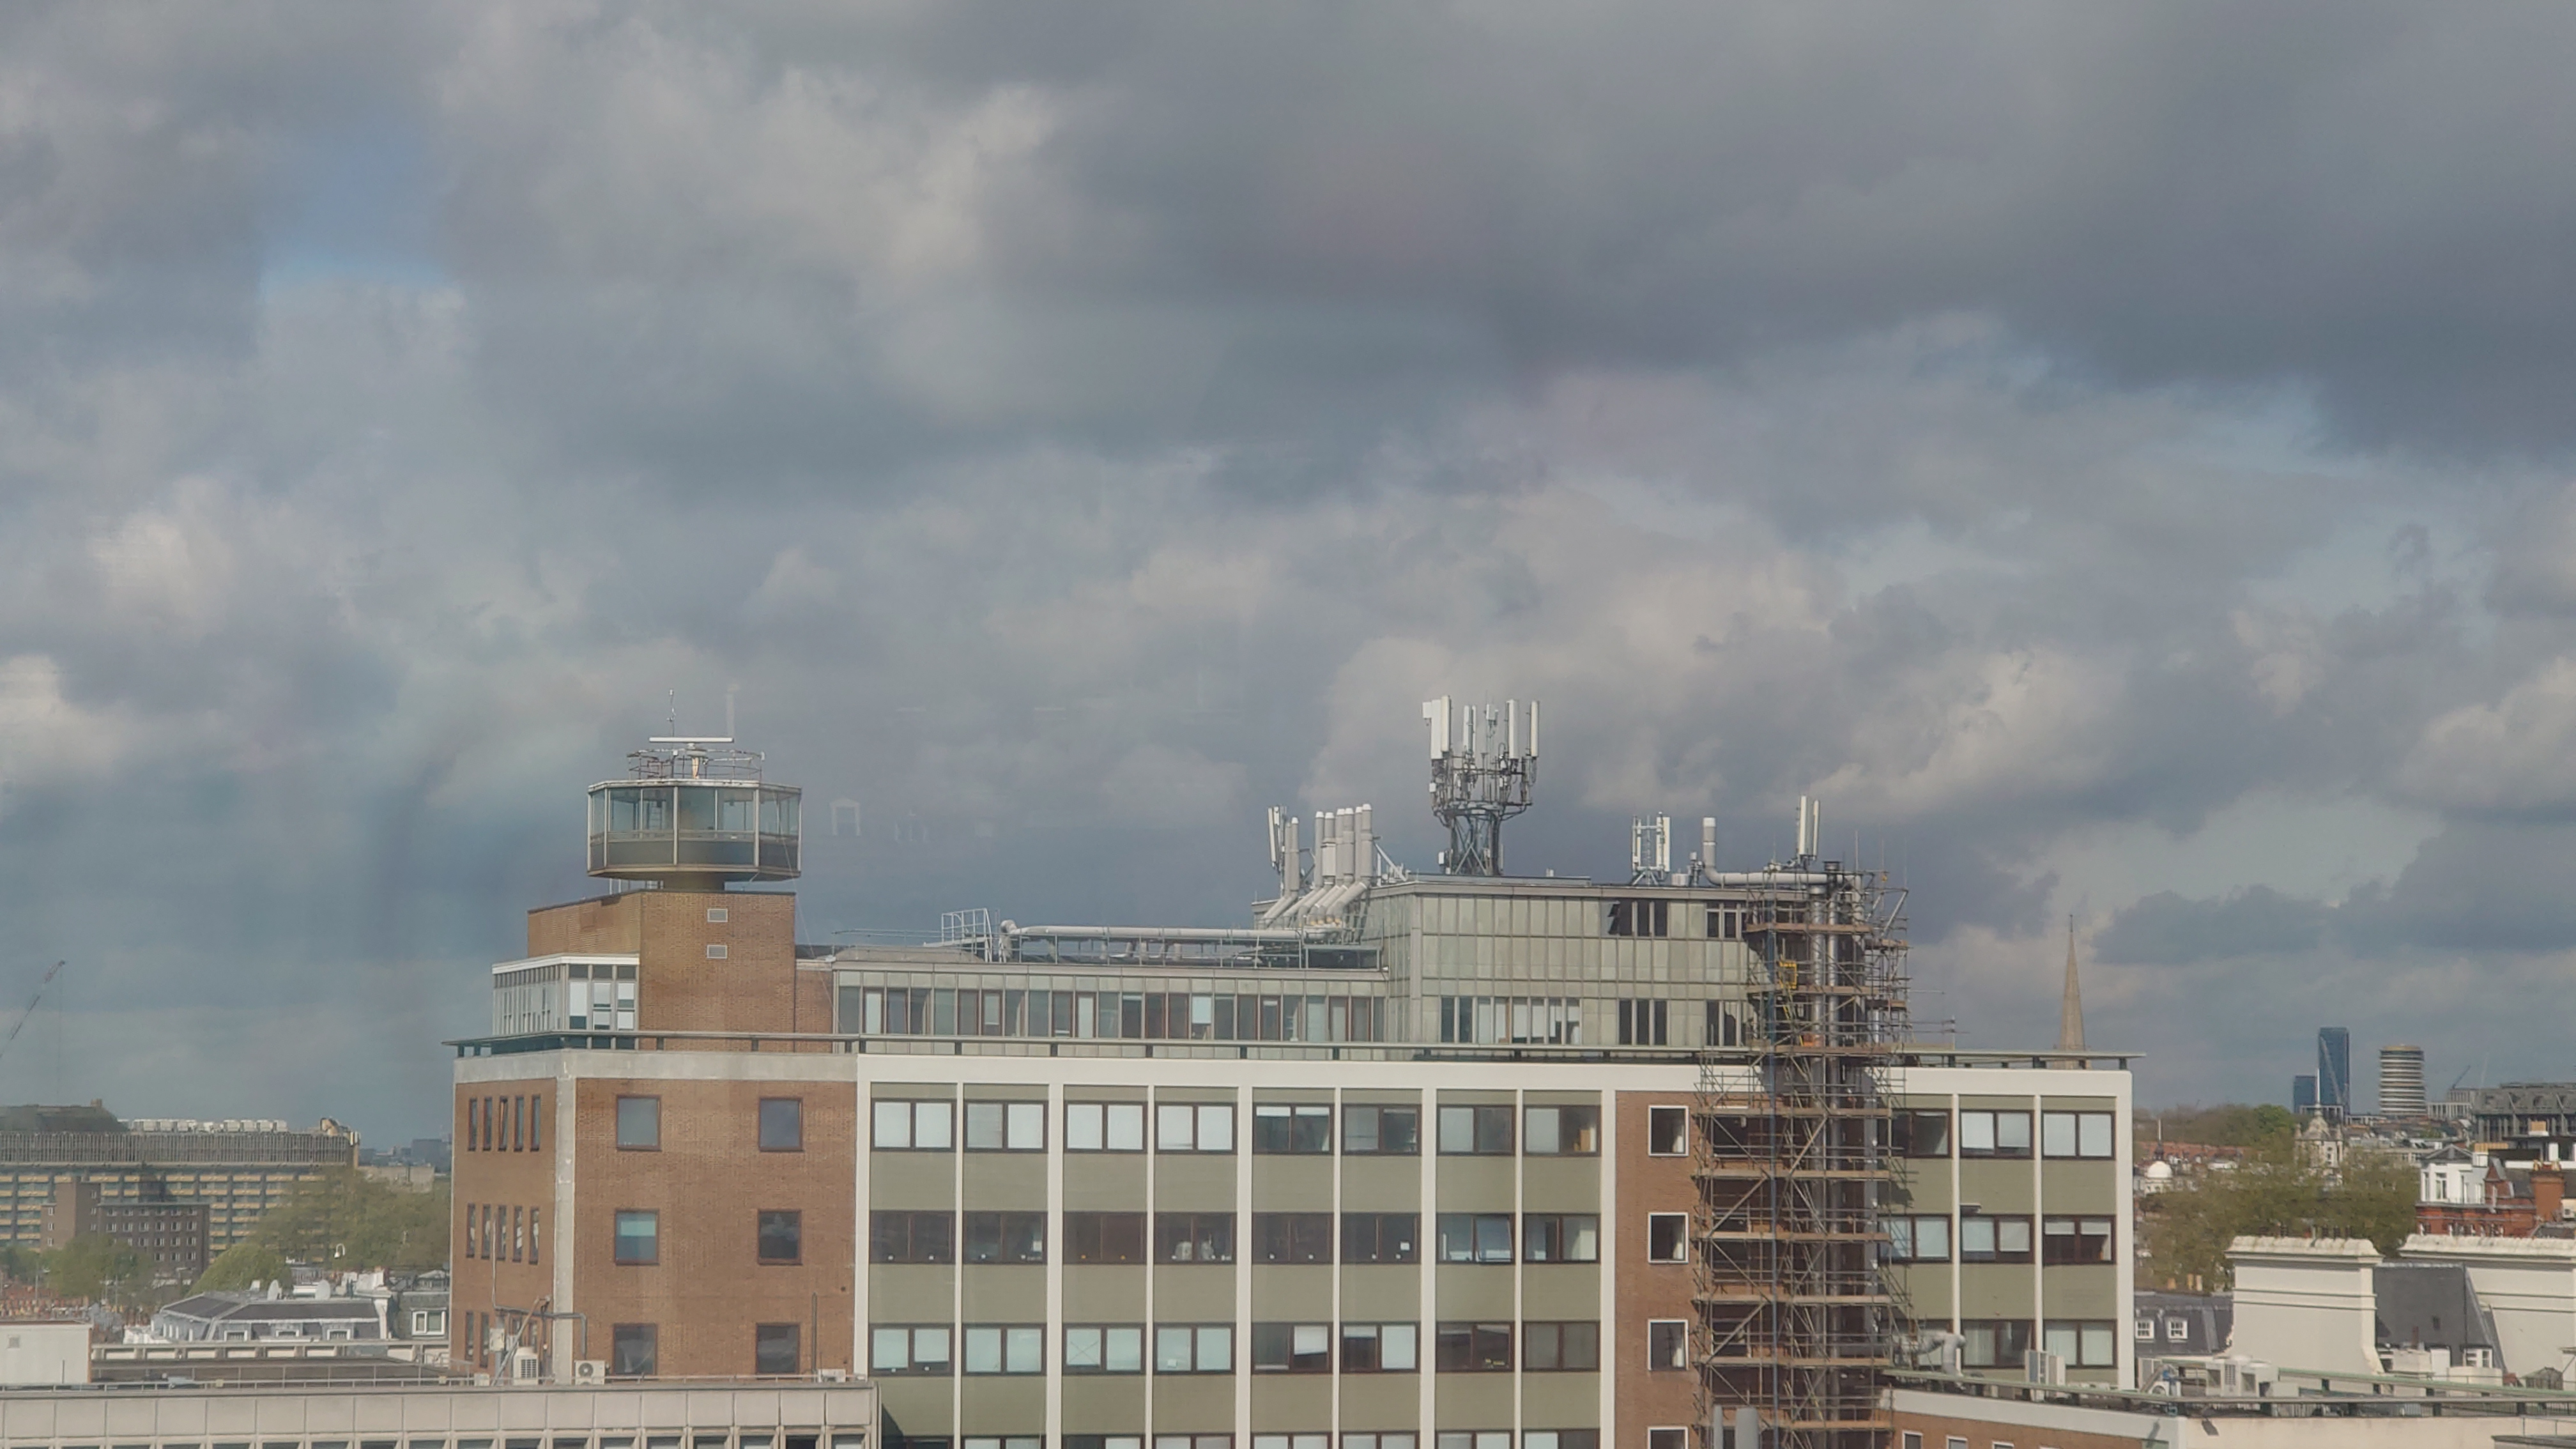
\includegraphics{../assets/viva/massive_mimo.jpg}
					}
				}
				\subfloat[Cellular statistics]{
					\resizebox{!}{3cm}{
						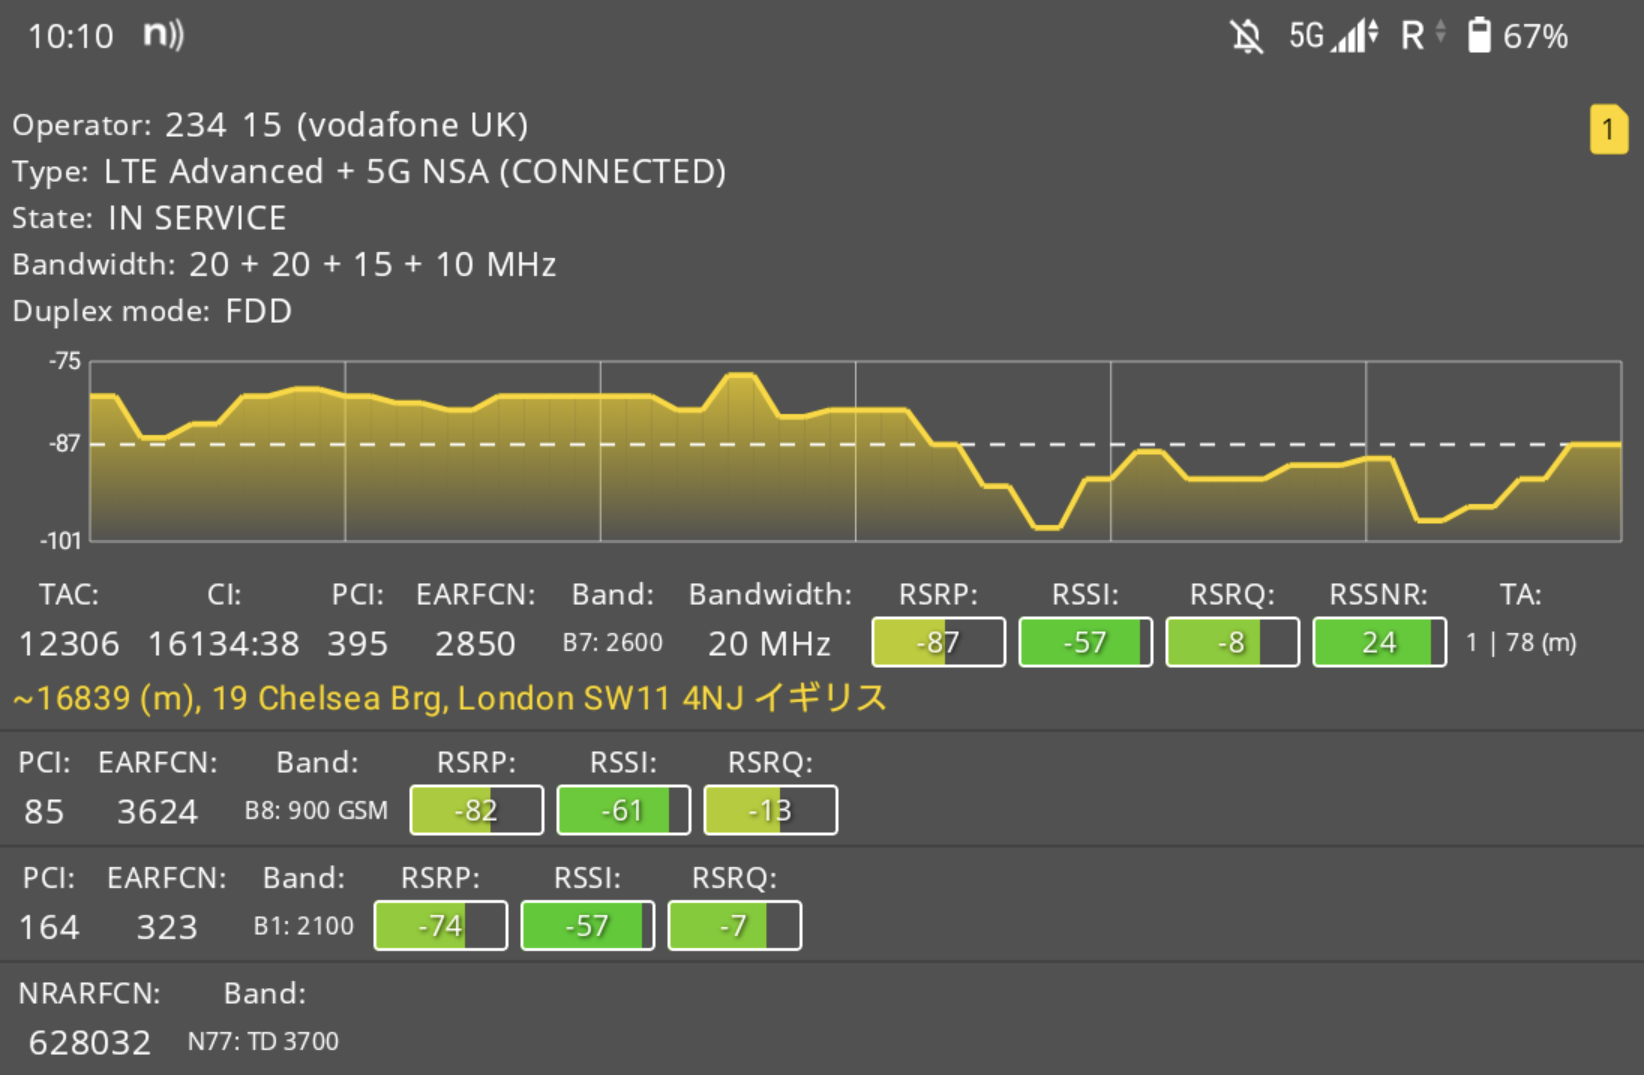
\includegraphics{../assets/viva/cellular_analysis.png}
					}
				}
			\end{figure}
		\end{block}
		\begin{block}{How far are we from the Shannon capacity?}
			\begin{equation*}
				C(\mathbf{H}) = \max_{\mathbf{Q} \succeq 0, \mathrm{tr}(\mathbf{Q}) \le P} \log \det \left( \mathbf{I} + \rho \mathbf{H} \mathbf{Q} \mathbf{H}^\mathsf{H} \right)
			\end{equation*}
			\vspace{-1em}
			\begin{itemize}
				\item Modulation, coding, and beamforming to \textcolor{gray}{adapt to} the stochastic channel
				\item \gls{ris} can \textcolor{blue}{shape and control} the channel
			\end{itemize}
		\end{block}
	\end{frame}

	\begin{frame}{What is \glsfmtshort{ris}?}
		A planar surface of controllable scattering elements for signal amplitude and phase manipulation \cite{Wu2020}.
		\begin{figure}
			\centering
			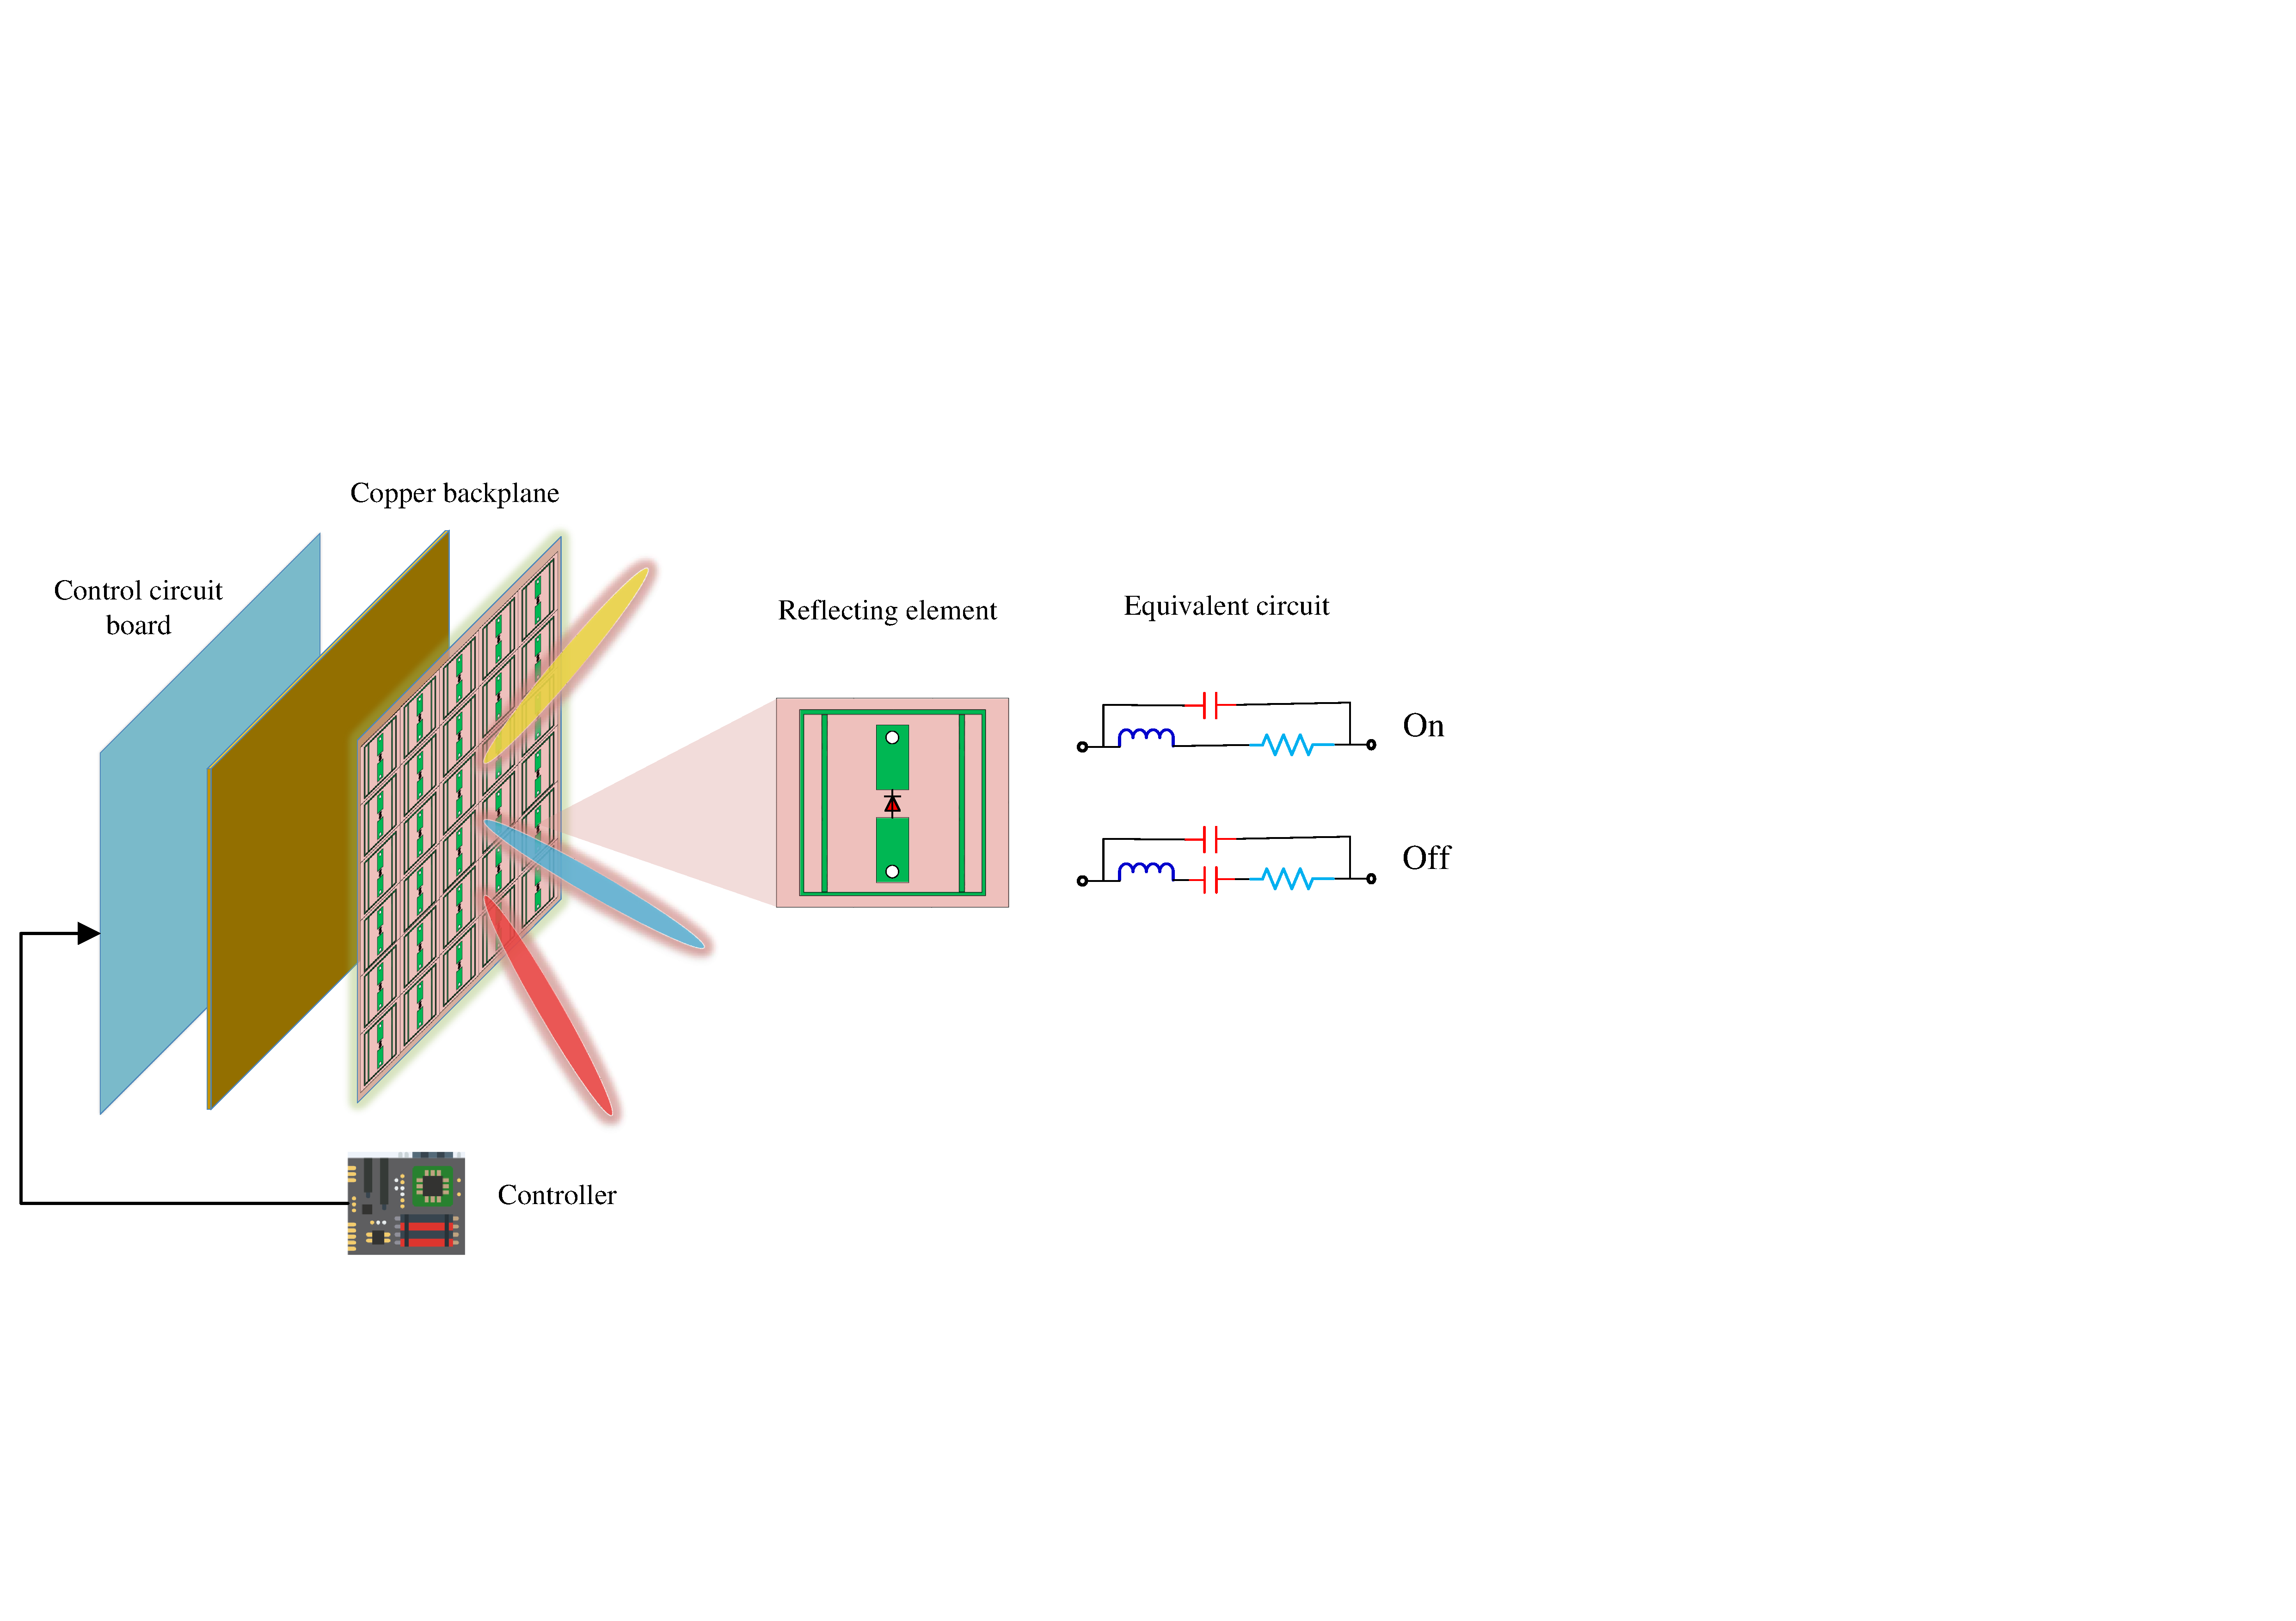
\includegraphics[width=0.65\textwidth]{../assets/viva/ris_architecture.pdf}
			\label{fg:ris_architecture}
		\end{figure}
		\begin{block}{Characteristics}
			\begin{itemize}
				\item Low-power and low-cost
				\item Negligible noise and latency
				\item Full-duplex without self-interference
				\item Programmable in real-time
			\end{itemize}
		\end{block}
	\end{frame}

	\begin{frame}{Ancestor of \glsfmtshort{ris}: Reflectarray antenna}
		% not parabolic with parallel phase front
		A reflectarray antenna consists of an array illuminated by a feeding antenna \cite{Deng2016}.
		\begin{figure}
			\centering
			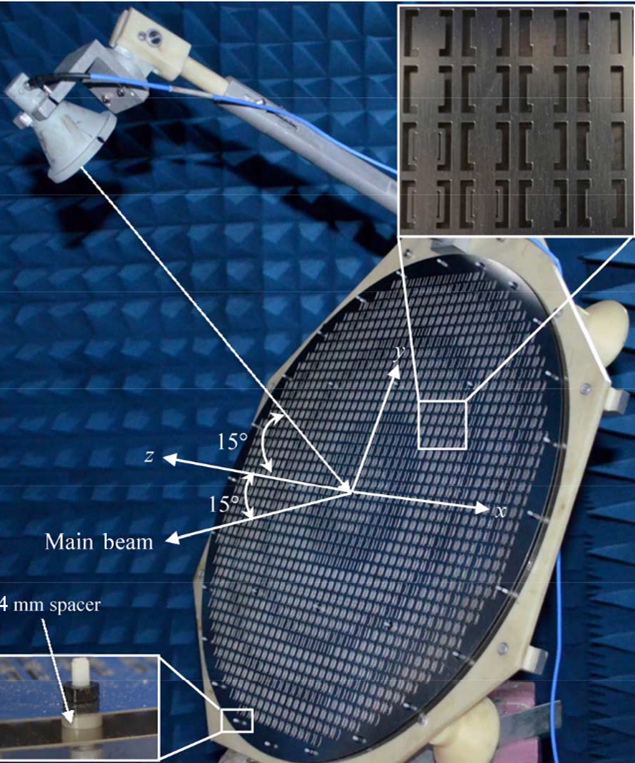
\includegraphics[width=0.45\textwidth]{../assets/viva/reflectarray.png}
		\end{figure}
		A progressive phase shift can be applied to the unit cells (a.k.a. elements) to steer the beam direction.
	\end{frame}

	\begin{frame}{What is the difference in \glsfmtshort{ris}?}
		\begin{enumerate}
			\item Metamaterial enables \textcolor{blue}{real-time control} and \textcolor{blue}{unconventional bahavior}.
			\item Impinging waves can be \textcolor{blue}{partially refracted and reflected}.
			\item The feed can be \textcolor{blue}{mobile} while the surface is \textcolor{blue}{scalable and multi-functional}.
			\item Elements can be physically interconnected for \textcolor{blue}{cooperative wave scattering}.
		\end{enumerate}
		\begin{exampleblock}{Refraction}
			\begin{columns}[T]
				\begin{column}{.25\textwidth}
					\begin{figure}
						\centering
						\resizebox{\columnwidth}{!}{
							\tikzstyle{glass}=[color=red!10]
\tikzset{
	light beam/.style={decoration={markings,
					mark=at position 0.5 with {\arrow[xshift=3pt]{latex}}},
			postaction={decorate}},
	light beam/.default=0.5}


% REFLECTION & REFRACTION
\begin{tikzpicture}
	\def\w{3.2}     % width interface
	\def\d{1}     % distance between source and glass
	\def\l{3.5}     % distance from glass
	\def\t{2}     % thickness glass
	% \def\na{1.0}  % air
	% \def\ng{2}    % glass
	\def\n{-1.5}

\begin{scope}[rotate=90]
	% MEDIUM
	\coordinate (L) at (-\w,-\d);              % lower-left point interface
	\fill[glass] (L) rectangle++ (2*\w,-\t);   % glass

% 	\foreach \anga in {-30,-20,...,30} {
	\foreach \anga in {-30,0,...,30} {
		\pgfmathsetmacro{\angg}{asin(\n*sin(\anga))}

		\pgfmathsetmacro{\a}{\d/cos(\anga)}
		\pgfmathsetmacro{\b}{\t/cos(\angg)}
		\pgfmathsetmacro{\c}{\l/cos(\anga)}

		\coordinate (S) at (0,0);                         % ray source
		\coordinate (I) at (\anga-90:\a);                 % impinging point
		\coordinate (O) at ($(I) + ({\angg-90}:\b)$);     % departing point
		\coordinate (E) at ($(O) + ({\anga-90}:\c)$);     % refraction tail

		% LINES
		\draw[light beam,thick] (S) -- (I);    % incoming ray
		\draw[light beam,thick] (I) -- (O);     % refracted ray in glass
		\draw[light beam,thick] (O) -- (E);     % refracted ray in air
	}
	\node at (-2.6,-2) {$n=-2/3$};
\end{scope}
\end{tikzpicture}

						}
					\end{figure}
				\end{column}
				% \hfill
				\begin{column}{.6\textwidth}
					\vspace{0.5cm}
					\begin{itemize}
						\item Negative index material can focus waves
						\item Amplitude and phase responses can be tuned by diodes and \glsfmtshort{fpga}
						\item Similar for wave reflection
					\end{itemize}
				\end{column}
			\end{columns}
		\end{exampleblock}
		\begin{exampleblock}{Reflection}
			\vspace{-1cm}
			\begin{figure}[H]
				\centering
				\subfloat[Incident wave\label{fg:wave_incident}]{
					\resizebox{!}{2.02cm}{
						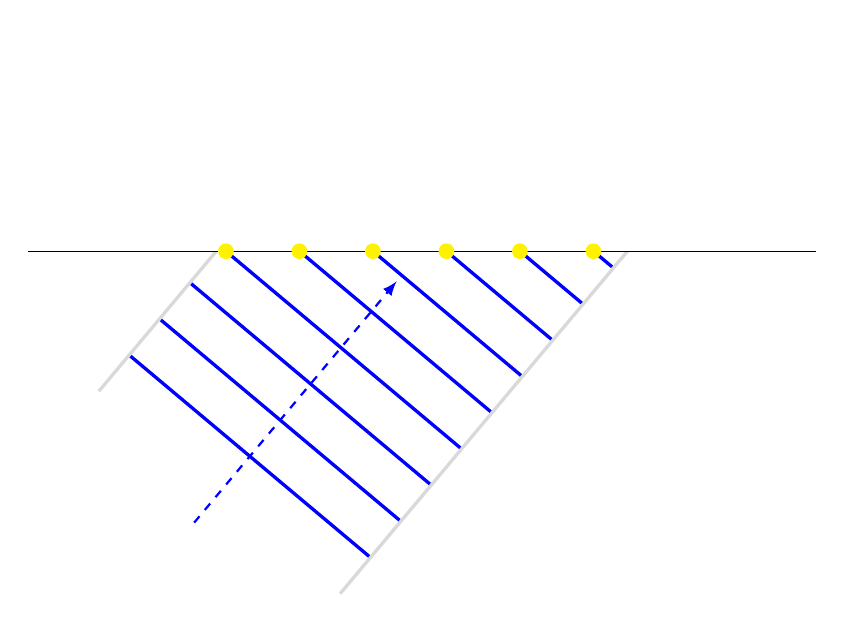
\begin{tikzpicture}[pics/v/.style={code={\draw (0,-#1) -- (0,#1);}}]
	\begin{scope}
		\clip[overlay] (-5,-5) rectangle (5,0);
		\path[rotate=140,overlay=false,very thick]
		foreach \x in {0,...,9}
			{(-2,-2+0.6*\x) coordinate (L\x) edge[	blue,name path global=p\x] ++ (4,0) coordinate (R\x)}
		(-2,-2) edge[gray!30] ++(0,6)
		(2,-2) edge[gray!30] ++(0,6)
		%    (0,-2) edge[gray!30] ++(0,7)
		(0,4.5) edge[blue,thick,dashed,-latex] ++ (0,-4);
	\end{scope}
	%  \begin{scope}
	%   \clip[overlay] (-5,0) rectangle (5,-5);
	%   \pgfmathsetmacro{\myx}{2*cos(20)/cos(30)}
	%   \path[rotate=200,overlay=false,very thick]
	%       foreach \x in {0,...,5}
	%     {(-\myx,0.8+0.4*\x) coordinate (L-\x) edge[green!70!black] ++ (2*\myx,0) coordinate (R-\x)}
	%    (-\myx,-2) edge[gray!30] ++(0,6)
	%    (\myx,-2) edge[gray!30] ++(0,6)
	%    (0,-2) edge[gray!30] ++(0,7)
	%    (0,3.6) edge[green!70!black,thick,dashed,latex-] ++ (0,-2);
	%  \end{scope}
	\path[name path=h] (-5,0) coordinate (L) -- (5,0) coordinate (R);
	\foreach \x in {1,2,3,4,5,6}
	\path[name intersections={of=h and p\x,by=i\x}] (i\x);
	%  \foreach \y in {1,...,\the\numexpr\x-1}
	%  {\pgfmathtruncatemacro{\myf}{50/(\x-\y)}
	%  \draw[thick,gray!\myf] (i\x) ++ (-0.18+\y*0.41,0)
	%     arc[start angle=0,end angle=-180,radius=-0.18+0.41*\y];}}
	\draw (L) -- (R);
	\path foreach \x in {1,2,3,4,5,6} {(i\x) node[circle,fill,yellow,inner sep=2pt]{}};
\end{tikzpicture}

					}
				}
				\subfloat[Reflected wave\label{fg:wave_reflected}]{
					\resizebox{!}{2cm}{
						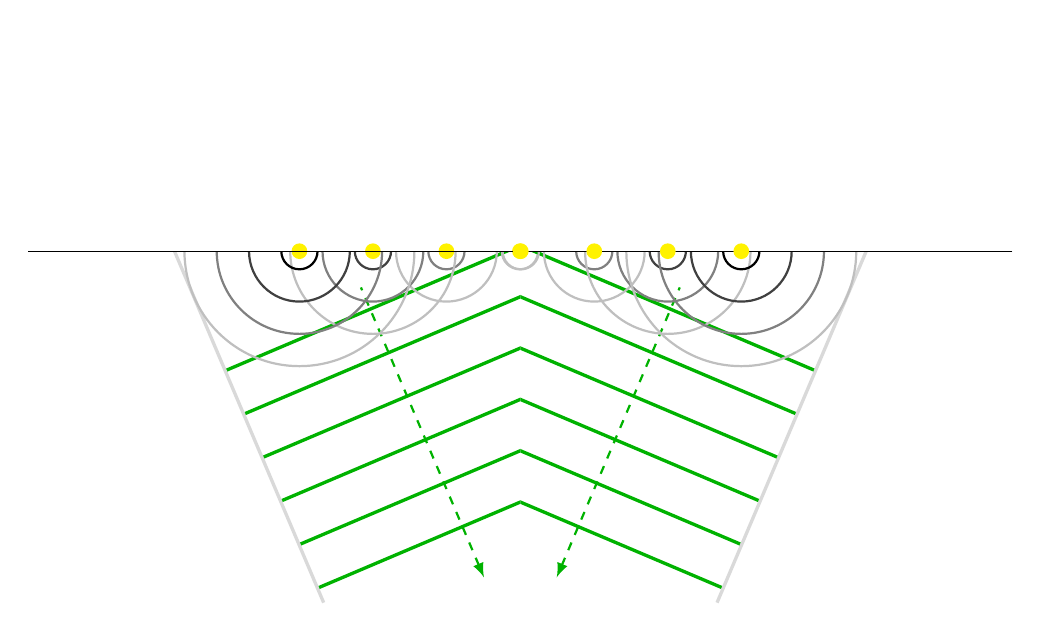
\begin{tikzpicture}[pics/v/.style={code={\draw (0,-#1) -- (0,#1);}}]
	\begin{scope}
		\clip[overlay] (-5,-5) rectangle (5,0);
		\path[rotate=140,overlay=false,very thick]
		foreach \x in {0,...,9}
			{(-2,-2+0.6*\x) coordinate (L\x) edge[blue,opacity=0,name path global=p\x] ++ (4,0) coordinate (R\x)};
	\end{scope}
	\begin{scope}[xshift=-0.97cm]
		\clip[overlay] (-5,0) rectangle (2.22,-5);
		\pgfmathsetmacro{\myx}{2*cos(30)/cos(30)}
		\path[rotate=203,overlay=false,very thick]
		foreach \x in {0,...,5}
			{(-\myx,0.8+0.6*\x) coordinate (L-\x) edge[green!70!black] ++ (2*\myx,0) coordinate (R-\x)}
		%    (-\myx,-2) edge[gray!30] ++(0,6)
		(\myx,-2) edge[gray!30] ++(0,6)
		%    (0,-2) edge[gray!30] ++(0,7)
		(0,4.5) edge[green!70!black,thick,dashed,latex-] ++ (0,-4);
	\end{scope}
	\path[name path=h] (-5,0) coordinate (L) -- (5,0) coordinate (R);
	\foreach \x in {2,3,4,5}
		{\path[name intersections={of=h and p\x,by=i\x}] (i\x);
			\foreach \y in {1,...,\the\numexpr\x-1}
				{
					\pgfmathtruncatemacro{\myf}{50*(\x-\y)}
					\draw[thick,gray!\myf] (i\x) ++ (-0.18+\y*0.41,0)
					arc[start angle=0,end angle=-180,radius=-0.18+0.41*\y];}}
	\draw (L) -- (R);
	\path foreach \x in {2,3,4,5} {(i\x) node[circle,fill,yellow,inner sep=2pt]{}};

	\begin{scope}[xscale=-1,xshift=-2.5cm]
		\begin{scope}
			\clip[overlay] (-5,-5) rectangle (5,0);
			\path[rotate=140,overlay=false,very thick]
			foreach \x in {0,...,9}
				{(-2,-2+0.6*\x) coordinate (L\x) edge[blue,opacity=0,name path global=p\x] ++ (4,0) coordinate (R\x)};
		\end{scope}
		\begin{scope}[xshift=-0.97cm]
			\clip[overlay] (-5,0) rectangle (2.22,-5);
			\pgfmathsetmacro{\myx}{2*cos(30)/cos(30)}
			\path[rotate=203,overlay=false,very thick]
			foreach \x in {0,...,5}
				{(-\myx,0.8+0.6*\x) coordinate (L-\x) edge[green!70!black] ++ (2*\myx,0) coordinate (R-\x)}
			%    (-\myx,-2) edge[gray!30] ++(0,6)
			(\myx,-2) edge[gray!30] ++(0,6)
			%    (0,-2) edge[gray!30] ++(0,7)
			(0,4.5) edge[green!70!black,thick,dashed,latex-] ++ (0,-4);
		\end{scope}
		\path[name path=h] (-5,0) coordinate (L) -- (5,0) coordinate (R);
		\foreach \x in {2,3,4,5}
			{\path[name intersections={of=h and p\x,by=i\x}] (i\x);
				\foreach \y in {1,...,\the\numexpr\x-1}
					{
						\pgfmathtruncatemacro{\myf}{50*(\x-\y)}
						\draw[thick,gray!\myf] (i\x) ++ (-0.18+\y*0.41,0)
						arc[start angle=0,end angle=-180,radius=-0.18+0.41*\y];}}
		\draw (L) -- (R);
		\path foreach \x in {2,3,4,5} {(i\x) node[circle,fill,yellow,inner sep=2pt]{}};
	\end{scope}

\end{tikzpicture}

					}
				}
			\end{figure}
		\end{exampleblock}
	\end{frame}

	\begin{frame}{Use case: Beamforming}
		% \textcolor{blue}{Joint beamforming} design of \gls{ris} and transceiver for a specific performance measure \cite{Wu2020}.
		% \gls{ris} and transceiver \textcolor{blue}{joint beamforming} design for a specific performance measure \cite{Wu2020}.
		\textcolor{blue}{Beamforming} of \gls{ris} and transceiver can be jointly designed for a specific performance measure \cite{Wu2020}.
		\begin{figure}
			\centering
			\subfloat[Coverage extension]{
				\resizebox{!}{2.75cm}{
					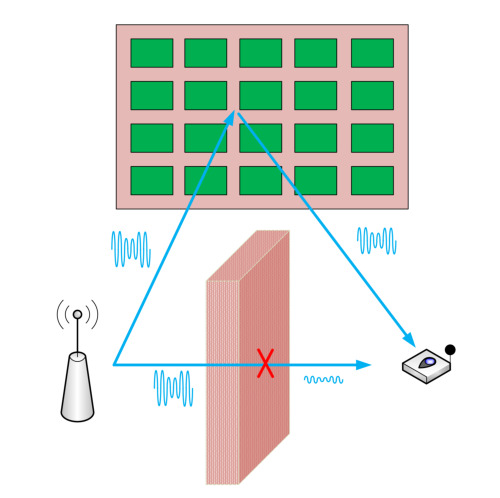
\includegraphics{../assets/viva/ris_beamforming_coverage.jpg}
				}
			}
			\subfloat[Security enhancement]{
				\resizebox{!}{2.75cm}{
					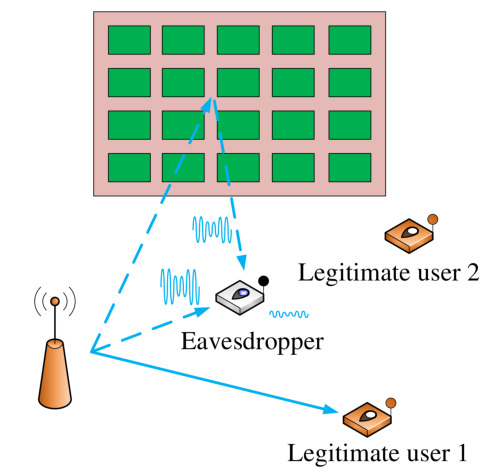
\includegraphics{../assets/viva/ris_beamforming_security.jpg}
				}
			}
			\subfloat[Interference mitigation]{
				\resizebox{!}{2.75cm}{
					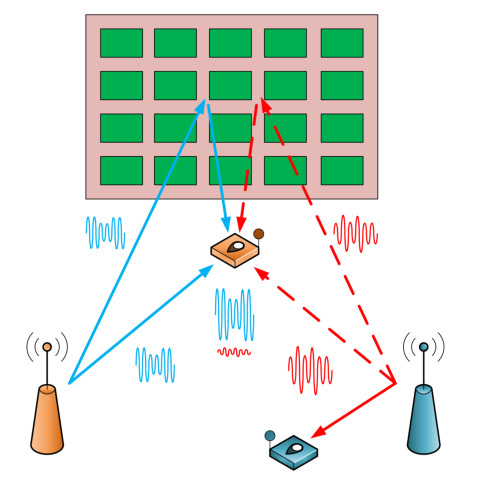
\includegraphics{../assets/viva/ris_beamforming_interference.jpg}
				}
			}
			\\
			\subfloat[Assist \glsfmtshort{d2d} network]{
				\resizebox{!}{2.75cm}{
					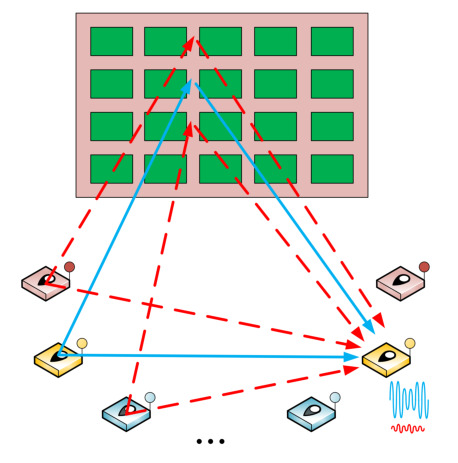
\includegraphics{../assets/viva/ris_beamforming_network.jpg}
				}
			}
			\subfloat[Assist information and power transfer]{
				\resizebox{!}{2.75cm}{
					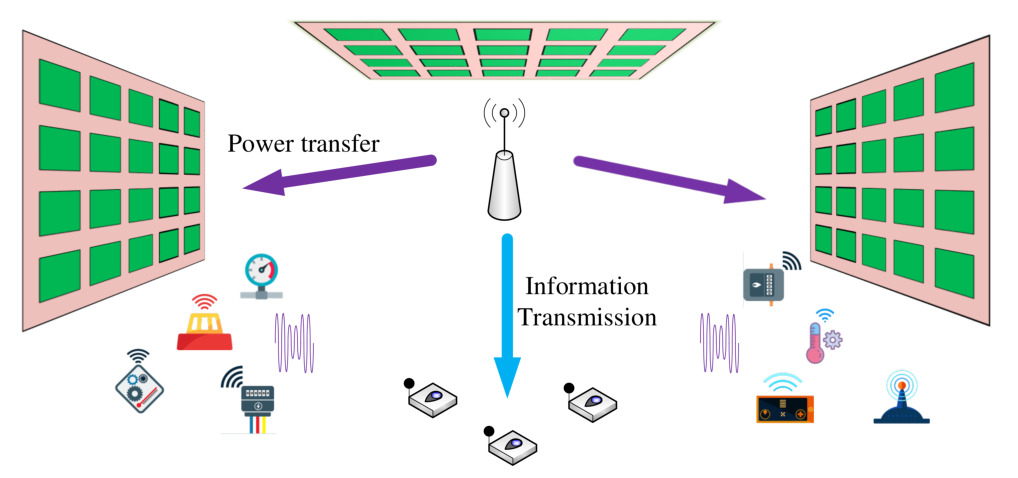
\includegraphics{../assets/viva/ris_beamforming_swipt.jpg}
				}
			}
		\end{figure}
	\end{frame}

	\begin{frame}{Use case: Modulation}
		\gls{ris} can be used for backscatter \textcolor{blue}{modulation} by periodically switching the reflection pattern \cite{Hu2021a}.
		\begin{figure}
			\centering
			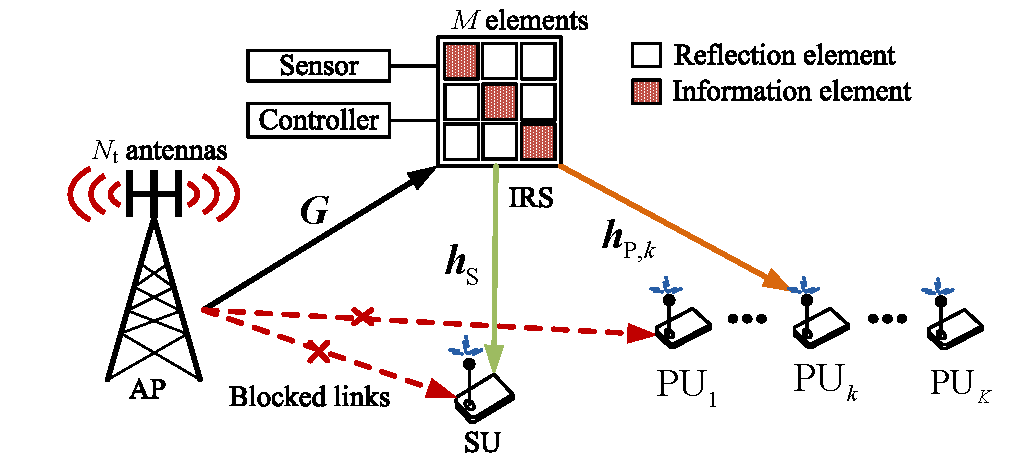
\includegraphics[width=0.9\textwidth]{../assets/viva/ris_modulation.pdf}
		\end{figure}
	\end{frame}

	\begin{frame}{Use case: Channel shaping}
		\textcolor{blue}{Channel shaping} exploits the \gls{ris} as a stand-alone device to modify the inherent properties of the propagation environment \cite{Arslan2022}.
		\begin{figure}
			\centering
			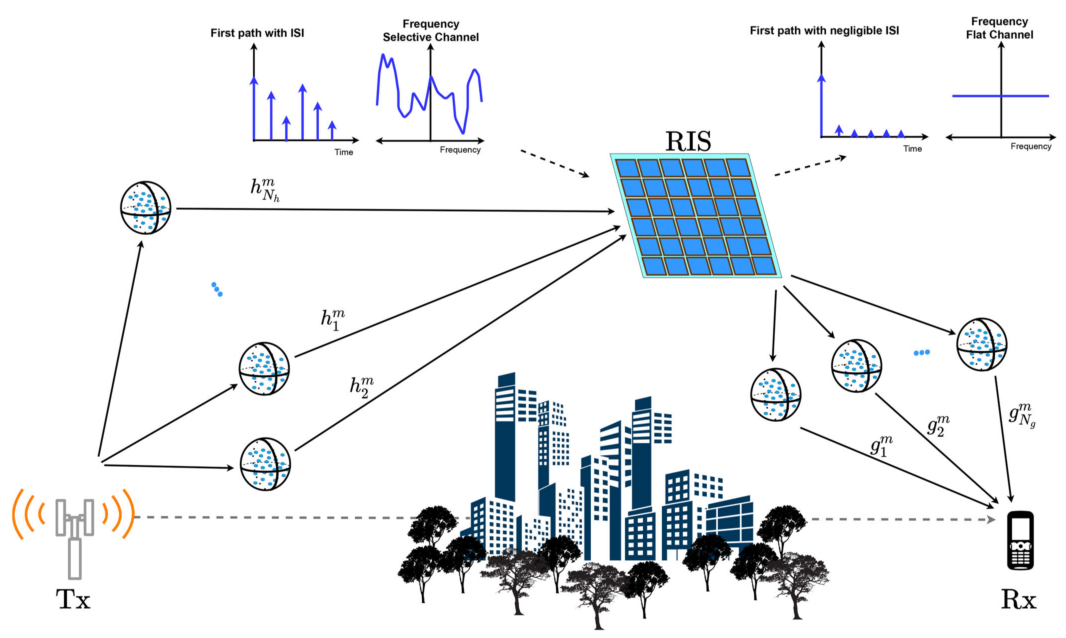
\includegraphics[width=0.9\textwidth]{../assets/viva/ris_shaping.pdf}
		\end{figure}
	\end{frame}
\end{section}

\begin{section}{Beamforming: \glsfmtshort{ris}-Aided \glsfmtshort{swipt}}
	\begin{frame}{\glsfmtshort{ris}-aided \glsfmtshort{swipt}: Joint waveform and beamforming design}
		\begin{block}{Overview}
			\begin{itemize}\setlength\itemsep{20pt}
				\item \textit{What does this paper propose?}

				A single-user multi-carrier \gls{swipt} system aided by a passive \gls{ris}.
				\item \textit{How does it differ from previous work?}

				We consider waveform and beamforming design for practical receiver architectures under non-linear harvester and frequency-flat \gls{ris} models.
				\item \textit{What are the benefits?}

				It exploits the spatial-frequency domain and rectifier behavior to enlarge the \gls{r-e} region, achieving squared asymptotic performance than conventional designs.
			\end{itemize}
		\end{block}
	\end{frame}

	\begin{frame}{\glsfmtshort{wpt} via radio waves}
		\vspace{-0.5cm}
		\begin{table}
			\footnotesize
			\rowcolors{2}{gray!25}{white}
			\renewcommand{\arraystretch}{1.25}
			\resizebox{\linewidth}{!}{
				\begin{tabular}{c c c c c c}
					\toprule
					% \hiderowcolors
					Categories                   & Medium                     & Device                     & Power level                            & Frequency                                & Range                     \\ \midrule
					% \showrowcolors
					                             & Magnetic resonant coupling & Resonators                 & Up to \SI{10}{\W}                      & \si{\kHz} -- \si{\MHz}                   & \si{\m}                   \\
					\cellcolor{white}            & Inductive coupling         & Wire coils                 & Up to \SI{10}{\W}                      & \si{\Hz} -- \si{\MHz}                    & \si{\cm}                  \\
					\multirow{-3}{*}{Near-field} & Capacitive coupling        & Metal plates               & Up to \SI{1}{\W}                       & \si{\kHz} -- \si{\MHz}                   & \si{\mm}                  \\
					\cellcolor{white}            & \textcolor{blue}{\gls{rf} wave}  & \textcolor{blue}{Rectenna} & \textcolor{blue}{\si{\uW} -- \si{\mW}} & \textcolor{blue}{\si{\MHz} -- \si{\GHz}} & \textcolor{blue}{\si{\m}} \\
					\multirow{-2}{*}{Far-field}  & Light wave                 & Laser                      & \si{\uW} -- \si{\mW}                   & \si{\THz}                                & \si{\km}                  \\ \bottomrule
				\end{tabular}
			}
		\end{table}
		\vspace{-0.25cm}
		\begin{figure}[H]
			\centering
			\resizebox{\columnwidth}{!}{
				\begin{circuitikz}[transform shape,align=center]
	\draw(0,0) node[draw](rf){\gls{rf}\\source};
	\draw(rf.east) node[txantenna]{};
	\draw(1,1) node{Tx};
	\draw(4.875,2) node[draw]{\textcolor{orange}{\gls{ris}}};
	\draw(4.875,1) node[draw]{\textcolor{orange}{Channel}};
	\draw(10,0) node[draw](mc){Matching\\network};
	\draw(mc.west) node[rxantenna,xscale=-1]{};
	\draw(8.7,1) node{Rx};
	\draw(mc.east) to ++(0.85,0) node[anchor=west,draw](r){\textcolor{blue}{Rectifier}};
	% \draw(d.east) to ++(0.85,0) node[anchor=west,draw](r){Low-pass\\filter};
	\draw(r.east) to ++(1,0) node[anchor=west,draw](dd){\gls{dc}-\gls{dc}\\converter};
	\draw(dd.east) to ++(1,0) node[anchor=west,draw](s){Storage};

	\draw [dashed] (-0.95,-0.75) rectangle (3.75,2.75);
	\draw (1.4,3) node[]{Energy transmitter};
	\draw [dotted] (6.25,-0.5) rectangle (13.2,2.5);
	\draw (9.9,2) node[]{\textcolor{blue}{Rectenna}};
	\draw [dotted] (13.8,-0.5) rectangle (19.9,1.25);
	\draw (16.75,0.875) node[]{Power management unit};
	\draw [dashed] (6,-0.75) rectangle (20.1,2.75);
	\draw (13.375,3) node[]{Energy receiver};

	\draw (-0.95,-1) node[]{$P_{\mathrm{DC}}^{\mathrm{T}}$};
	\draw (3.75,-1) node[]{$P_{\mathrm{RF}}^{\mathrm{T}}$};
	\draw (6,-1) node[]{$P_{\mathrm{RF}}^{\mathrm{R}}$};
	\draw (13.5,-1) node[]{$P_{\mathrm{DC}}^{\mathrm{R}}$};
	\draw (20.3,-1) node[]{$P_{\mathrm{DC}}^{\mathrm{S}}$};

	\draw[gray,dashdotted,-latex] (10.925,-0.5) to ++(0,-1.5) to ++(-1,0) node[anchor=east,draw](c){Channel\\feedback};
	\draw[gray,dashdotted,latex-] (1.4,-0.75) to ++(0,-1.25) to ++(1,0) node[anchor=west,draw](s){Signal\\optimization};
	\draw[gray,dashdotted,-latex] (c.west) to (s.east);
	\draw[gray] (6.45,-2) node[]{Reverse\\communication link};
\end{circuitikz}

			}
			\label{fg:wpt_architecture}
		\end{figure}
		\vspace{-1em}
		The end-to-end \gls{wpt} efficiency is
		\begin{equation*}
			\eta = \frac{P_{\mathrm{DC}}^\mathrm{S}}{P_{\mathrm{DC}}^\mathrm{T}} = \underbrace{\frac{P_{\mathrm{RF}}^\mathrm{T}}{P_{\mathrm{DC}}^\mathrm{T}}}_{\eta_1} \textcolor{orange}{\underbrace{\frac{P_{\mathrm{RF}}^\mathrm{R}}{P_{\mathrm{RF}}^\mathrm{T}}}_{\eta_2}} \textcolor{blue}{\underbrace{\frac{P_{\mathrm{DC}}^\mathrm{R}}{P_{\mathrm{RF}}^\mathrm{R}}}_{\eta_3}} \underbrace{\frac{P_{\mathrm{DC}}^\mathrm{S}}{P_{\mathrm{DC}}^\mathrm{R}}}_{\eta_4}
		\end{equation*}
		where $\eta_2$ and $\eta_3$ models the channel and rectenna, respectively.
	\end{frame}

	\begin{frame}{Received signal and harvested power}
		The rectenna efficiency $\eta_3$ depends on its input waveform (power and shape).
		\begin{block}{Rectenna model}
			% \vspace{-0.25cm}
			% \begin{figure}[H]
			% 	\centering
			% 	\subfloat[Rectenna]{
			% 		\resizebox{0.35\columnwidth}{!}{
			% 			\begin{circuitikz}[transform shape]
	\draw (0,0) to [sV=$v_{\mathrm{S}}$] (0,2);
	\draw (0,2) to [short] (1,2);
	\draw (1,2) to [generic,l=$Z_{\mathrm{A}}$] (3,2);
	\draw (3,2) to [short] (4,2);
	\draw (4,2) to [generic,l=$Z_{\mathrm{in}}$, v<=$v_{\mathrm{in}}$] (4,0);
	\draw (4,0) to [short] (2,0) node[ground](GND){};
	\draw (2,0) to [short] (0,0);
\end{circuitikz}

			% 		}
			% 		\label{fg:rectenna}
			% 	}
			% 	\subfloat[Half-wave rectifier]{
			% 		\resizebox{0.35\columnwidth}{!}{
			% 			\begin{circuitikz}[transform shape]
	\draw (0,0) to [sV=$v_{\mathrm{in}}$] (0,2);
	\draw (0,2) to [short] (0.25,2);
	\draw (0.25,2) to [D, v<=$v_{\mathrm{D}}$] (2.25,2);
	\draw (2.25,2) to [short, -*] (2.5,2);
	\draw (2.5,2) to [C, l_=$C$, -*] (2.5,0);
	\draw (2.5,2) to [short] (4.25,2);
	\draw (4.25,2) to [R=$R_{\mathrm{L}}$, v=$v_{\mathrm{out}}$] (4.25,0);
	\draw (4.25,0) to [short] (2,0) node[ground](GND){};
	\draw (2,0) to [short] (0,0);
\end{circuitikz}

			% 		}
			% 		\label{fg:halfwave_rectifier}
			% 	}
			% \end{figure}
			% \vspace{-0.25cm}
			\begin{itemize}
				\item Linear region (constant $\eta_3$): $P_{\mathrm{DC}}^\mathrm{R} = \eta_3 P_\mathrm{RF}^\mathrm{R} = \eta_3 \mathbb{A}\bigl\{ \lvert y(t) \rvert^2 \bigr\}$
				\item Non-linear region: Taylor expansion on diode characteristic equation
				\vspace{-0.25cm}
				\begin{equation*}
					\arg_{x(t)} \max P_{\mathrm{DC}}^\mathrm{R} = \arg_{x(t)} \max z \triangleq \sum_{i=2,\text{even}}^{n_0} \beta_i \mathbb{A}\bigl\{ y^i(t) \bigr\},
					\vspace{-0.5cm}
				\end{equation*}
				where $\beta_i = I_\mathrm{S} \frac{R_\mathrm{A}^{i/2}}{i!(n v_\mathrm{T})^i}$ is a constant and $n_0$ is the truncation order.
			\end{itemize}
		\end{block}
		\begin{alertblock}{In multi-carrier \glsfmtshort{wpt} \textellipsis}
			\begin{itemize}
				\item $n_0 \ge 4$ allows components to compensate each other for higher \gls{dc} power
				\item High \gls{papr} (e.g., multi-sine) is preferred \cite{Trotter2009}
			\end{itemize}
			\vspace{-0.5cm}
			\begin{figure}
				\centering
				\subfloat{
					\resizebox{!}{2.5cm}{
						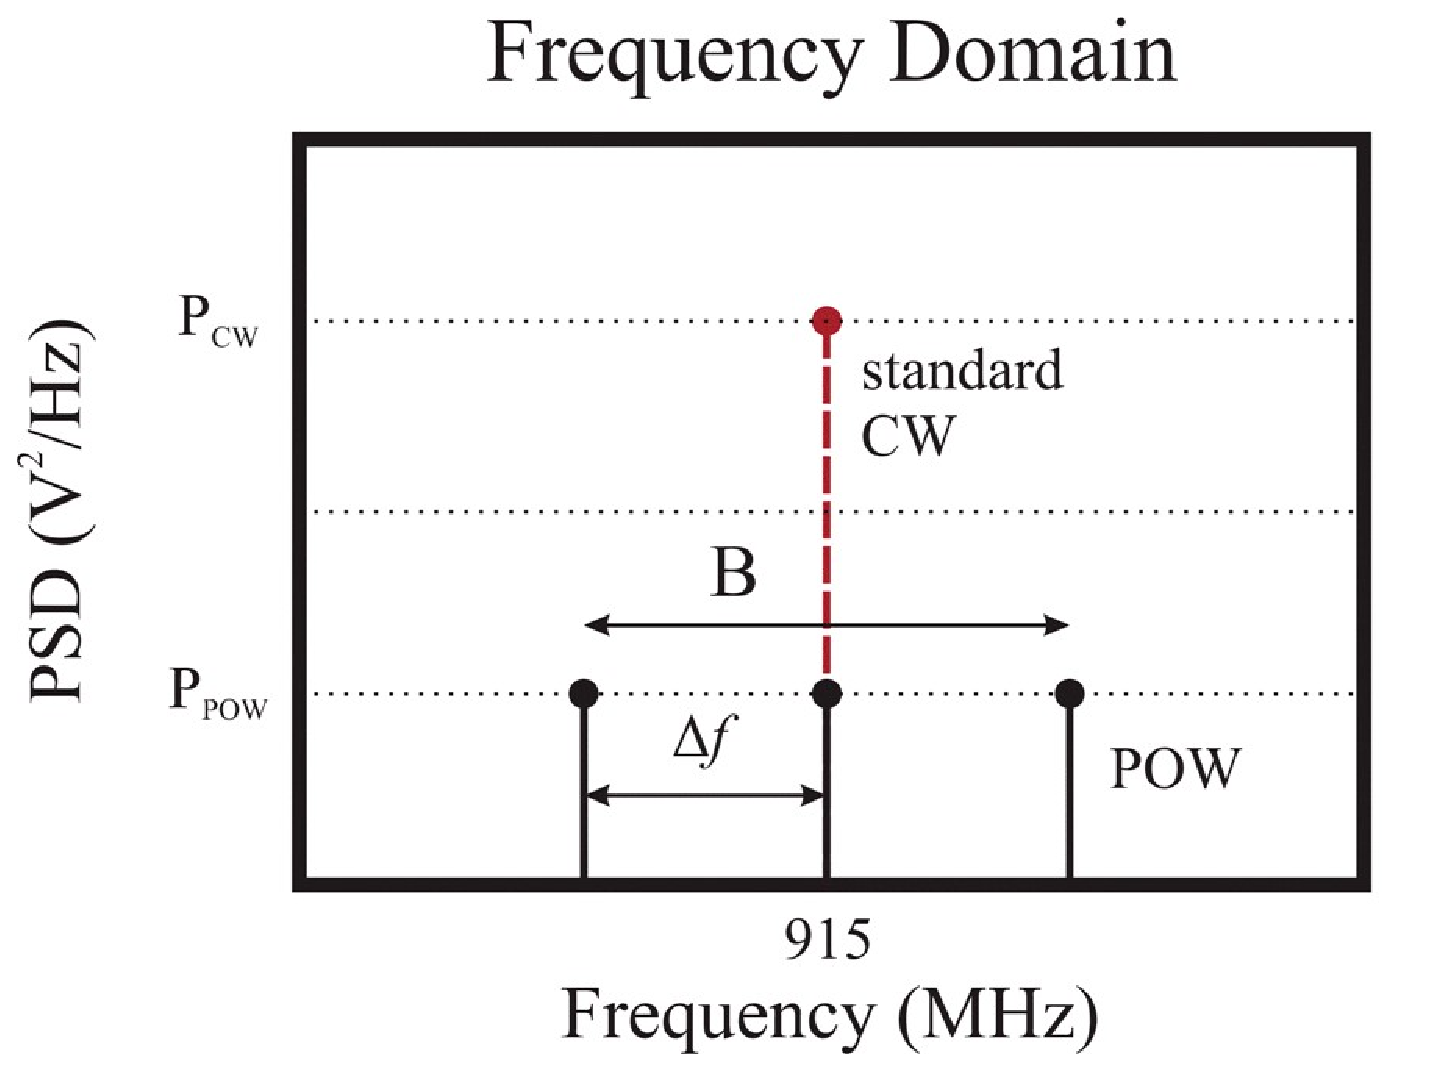
\includegraphics{../assets/viva/multisine_frequency_domain.eps}
					}
				}
				\subfloat{
					\resizebox{!}{2.5cm}{
						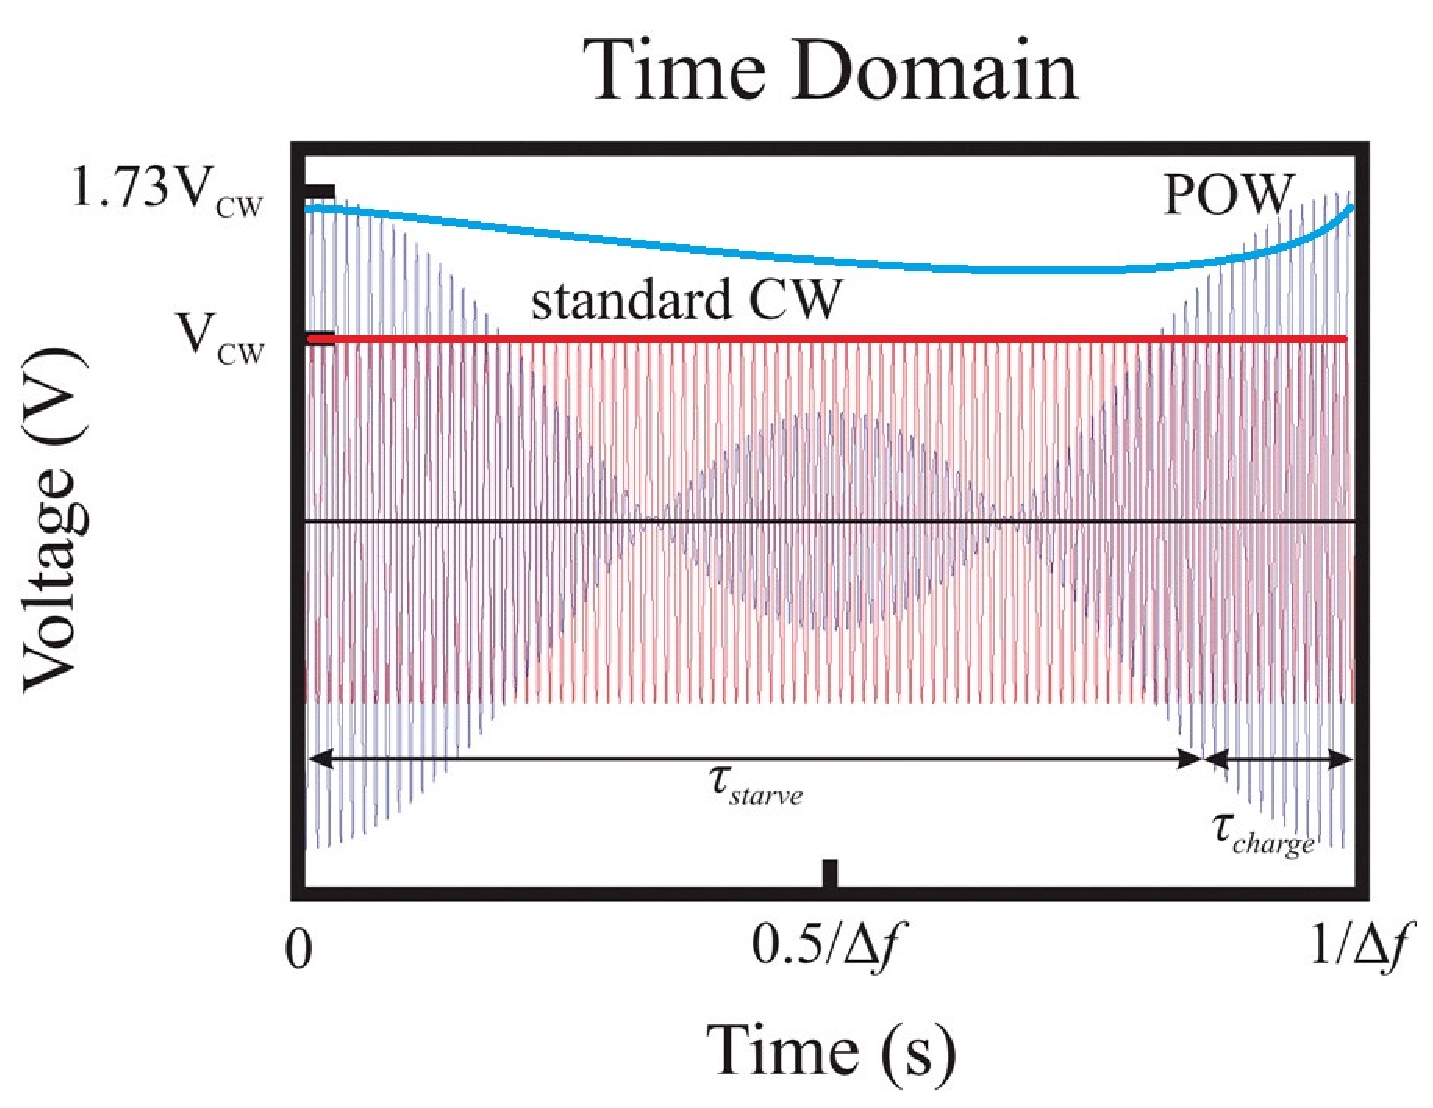
\includegraphics{../assets/viva/multisine_time_domain.eps}
					}
				}
			\end{figure}
		\end{alertblock}
	\end{frame}

	\begin{frame}{From \glsfmtshort{wpt} to \gls{ris}-aided \glsfmtshort{swipt}}
		\begin{figure}[H]
			\centering
			\def\svgwidth{0.5\columnwidth}
			\input{../assets/viva/system.eps_tex}
		\end{figure}

		\begin{itemize}
			\item \gls{swipt} features shared signal, spectrum, and infrastructure
			\item \gls{ris} enhances the RF-to-RF efficiency $\eta_2$ which has been a major concern
		\end{itemize}
		\begin{block}{Transmit waveform}
			\begin{equation*}
				\mathbf{x}(t) = \Re \left\{\sum_{n=1}^N \Bigl(\mathbf{w}_{\mathrm{I},n} \cdot \underbrace{\tilde{x}_{\mathrm{I},n}(t) e^{\jmath 2{\pi}{f_n}{t}}}_\text{modulated}+\mathbf{w}_{\mathrm{P},n} \cdot \underbrace{e^{\jmath 2{\pi}{f_n}{t}}}_\text{multi-sine}\Bigr) \right\}
			\end{equation*}
		\end{block}
		\begin{block}{Frequency-flat \glsfmtshort{ris} model}
			\begin{equation*}
				\mathbf{h}_{n}^\mathsf{H} = \mathbf{h}_{\mathrm{D},n}^\mathsf{H} + \mathbf{h}_{\mathrm{B},n}^\mathsf{H} \mathbf{\Theta} \mathbf{H}_{\mathrm{F},n}
			\end{equation*}
		\end{block}
	\end{frame}

	\begin{frame}{Performance analysis}
		\begin{block}{Receiver architectures}
			\vspace{-0.5cm}
			\begin{figure}
				\centering
				\subfloat[\gls{ts} receiver]{
					\resizebox{0.48\columnwidth}{!}{
						\begin{circuitikz}[transform shape,align=center]
	\draw (0,0) node[bareRXantenna](r){Rx}(r.center)
		to[short] ++(0,-1) node[below]{Time switcher}
		to[short] node[spdt,anchor=in](s){} ++(0.5,0);

	\draw (s.out 1)
		to ++(1.25,0)
		to ++(0,0.5)
		to ++(1,0) node[draw,minimum width=2.5cm,anchor=west](eh){Energy\\harvester};
	% \draw (eh.east) to ++(1,0) node[draw,anchor=west,minimum width=2.5cm]{Power\\management};

	\draw (s.out 2)
		to ++(1.25,0)
		to ++(0,-0.5)
		to ++(1,0) node[draw,anchor=west,minimum width=2.5cm]{Information\\decoder};
\end{circuitikz}

% \begin{circuitikz}[transform shape,align=center]
% 	\draw (0,0) node[bareRXantenna](r){Rx}(r.center)
% 		to[short] ++(0,-1)
% 		to node[coupler,anchor=left up](c){Power splitter} ++(1,0);
% 	\draw (c.right up)
% 		to[short] ++(0.5,0)
% 		to ++(0,0.5)
% 		to ++(1,0) node[draw,minimum width=2.5cm,anchor=west](eh){Energy\\harvester};
% 	\draw (eh.east) to ++(1,0) node[draw,anchor=west,minimum width=2.5cm]{Power\\management};
% 	\draw (c.right down)
% 		to[short] ++(0.5,0)
% 		to ++(0,-0.5)
% 		to ++(1,0) node[draw,anchor=west,minimum width=2.5cm]{Information\\decoder};
% \end{circuitikz}

					}
					\label{fg:receiver_ts}
				}
				\subfloat[\gls{ps} receiver]{
					\resizebox{0.48\columnwidth}{!}{
						\begin{circuitikz}[transform shape,align=center]
	\draw (0,0) node[bareRXantenna](r){Rx}(r.center)
		to[short] ++(0,-1)
		to node[coupler,anchor=left up](c){Power splitter} ++(1,0);
	\draw (c.right up)
		to[short] ++(0.5,0)
		to ++(0,0.5)
		to ++(1,0) node[draw,minimum width=2.5cm,anchor=west](eh){Energy\\harvester};
	% \draw (eh.east) to ++(1,0) node[draw,anchor=west,minimum width=2.5cm]{Power\\management};
	\draw (c.right down)
		to[short] ++(0.5,0)
		to ++(0,-0.5)
		to ++(1,0) node[draw,anchor=west,minimum width=2.5cm]{Information\\decoder};
\end{circuitikz}

					}
					\label{fg:receiver_ps}
				}
			\end{figure}
		\end{block}
		\begin{block}{\glsfmtfull{r-e} region of \glsfmtshort{ps}}
			\vspace{-0.25cm}
			\begin{align*}
				R(\boldsymbol{\theta},\mathbf{w}_{\mathrm{I}},\rho) &= \sum_{n=1}^N{\log_2\left(1+\frac{(1-\rho)\lvert \mathbf{h}_{n}^\mathsf{H}\mathbf{w}_{\mathrm{I},n} \rvert^2}{\sigma_n^2}\right)},\\
				z(\boldsymbol{\theta},\mathbf{w}_{\mathrm{I}},\mathbf{w}_{\mathrm{P}},\rho) &= \sum_{i=2,\text{even}}^{n_0}{\beta_i}{\rho^{i/2}}{\mathbb{E}\left\{\mathbb{A}\left\{y^i(t)\right\}\right\}},
			\end{align*}
			\begin{equation*}
				\mathcal{C}_\mathrm{R-E}(P)\triangleq \Bigl\{(r,e) : 0 \le r \le R, \ 0 \le e \le z, \lVert{\mathbf{W}_{\mathrm{I}}}\rVert _\mathrm{F}^2/2 + \lVert{\mathbf{W}_{\mathrm{P}}}\rVert _\mathrm{F}^2/2 \le P \Bigr\}
			\end{equation*}
		\end{block}
	\end{frame}

	\begin{frame}{Joint waveform and beamforming design}
		\begin{block}{Problem formulation}
			\vspace{-0.25cm}
			\begin{maxi*}
				{\scriptstyle{\boldsymbol{\theta},\mathbf{W}_\mathrm{I},\mathbf{W}_\mathrm{P},\rho}}{z(\boldsymbol{\theta},\mathbf{W}_\mathrm{I},\mathbf{W}_\mathrm{P},\rho)}{}{}
				\addConstraint{\lVert{\mathbf{W}_{\mathrm{I}}}\rVert _\mathrm{F}^2/2 + \lVert{\mathbf{W}_{\mathrm{P}}}\rVert _\mathrm{F}^2/2\le{P}}
				\addConstraint{R(\boldsymbol{\theta},\mathbf{W}_\mathrm{I},\rho) \ge \bar{R}}
				\addConstraint{\lvert{\phi_l}\rvert=1, \quad l=1,\dots,L}
				\addConstraint{0 \le \rho \le 1,}
			\end{maxi*}
		\end{block}
		\begin{exampleblock}{Solution by \glsfmtfull{bcd}}
			\begin{itemize}
				\item Optimally decouple the spatial and frequency domain design
				\begin{equation*}
					\mathbf{w}_{\mathrm{I/P}, n} = \underbrace{s_{\mathrm{I/P}, n}}_\text{frequency} \underbrace{\mathbf{p}_{\mathrm{I/P}, n}}_\text{spatial}
				\end{equation*}
				\item Active beamforming $\mathbf{p}$: \gls{mrt}
				\item Passive beamforming $\boldsymbol{\theta}$: \gls{sca}
				\item Power allocation $\mathbf{s}$ and splitting ratio $\rho$: \gls{gp}
			\end{itemize}
		\end{exampleblock}
	\end{frame}

	\begin{frame}{Simulation results: Number of subbands $N$}
		\begin{figure}
			\centering
			\subfloat[\gls{r-e} region]{
				\resizebox{0.45\columnwidth}{!}{
					% This file was created by matlab2tikz.
%
%The latest updates can be retrieved from
%  http://www.mathworks.com/matlabcentral/fileexchange/22022-matlab2tikz-matlab2tikz
%where you can also make suggestions and rate matlab2tikz.
%
\definecolor{mycolor1}{rgb}{0.00000,0.44700,0.74100}%
\definecolor{mycolor2}{rgb}{0.85000,0.32500,0.09800}%
\definecolor{mycolor3}{rgb}{0.92900,0.69400,0.12500}%
\definecolor{mycolor4}{rgb}{0.49400,0.18400,0.55600}%
\definecolor{mycolor5}{rgb}{0.46600,0.67400,0.18800}%
%
\begin{tikzpicture}

\begin{axis}[%
width=4.036in,
height=3.396in,
at={(0.677in,0.458in)},
scale only axis,
xmin=0,
xlabel style={font=\color{white!15!black}},
xlabel={Per-subband rate [bps/Hz]},
ymin=0,
ylabel style={font=\color{white!15!black}},
ylabel={DC [$\mu$A]},
axis background/.style={fill=white},
xmajorgrids,
ymajorgrids,
legend style={legend cell align=left, align=left, draw=white!15!black},
title style={font=\huge}, label style={font=\huge}, ticklabel style={font=\LARGE}, legend style={font=\LARGE}
]
\addplot [color=mycolor1, line width=2.0pt, mark=o, mark options={solid, mycolor1}]
  table[row sep=crcr]{%
10.0371541503521	2.22044604925031e-10\\
9.50888287931245	7.67218297348236\\
8.98061160969771	16.4035328868797\\
8.45234034327624	23.7184488015709\\
7.92406907805198	29.205421549582\\
7.3957978136944	33.108418398381\\
6.86752655715228	35.8060858943009\\
6.33925531456315	37.6402604405573\\
5.81098410797576	38.8754185210755\\
5.28271290103602	39.7025741932163\\
4.75444168414669	40.2547940715469\\
4.22617042980331	40.6229044735893\\
3.69789919151785	40.8681643325841\\
3.16962794157827	41.0316006620616\\
2.64135688073796	41.1405795757475\\
2.11308593958905	41.2133145315082\\
1.58481573162	41.2619161559168\\
1.05654557443832	41.2944351162874\\
0.52831621285643	41.3162247649014\\
0.0172895850115278	41.3305512860995\\
};
\addlegendentry{PS: $N = 1$}

\addplot [color=mycolor2, dashed, line width=2.0pt, mark=+, mark options={solid, mycolor2}]
  table[row sep=crcr]{%
9.02654522797361	2.22044604925031e-10\\
8.55146390059239	6.85672511413178\\
8.07638260779107	14.9052859902322\\
7.60130144663416	22.0060908430934\\
7.12622060328784	27.6704698672712\\
6.65114024798395	32.0013219513062\\
6.17606060075074	35.260704866419\\
5.70098161136798	37.7089802785193\\
5.22590380097997	39.5578388388224\\
4.75082663535468	40.9688790179793\\
4.27575311838366	42.0598435792836\\
3.80068610434027	42.9182097430551\\
3.32564099290071	43.6116792643263\\
2.85063913633349	44.1927578797524\\
2.37567922919448	44.6914808377669\\
1.90064908156813	45.0988588665419\\
1.42547871463989	45.3685552024517\\
0.950295873559429	45.5091782183481\\
0.475137711619894	45.5794354570947\\
0.000663657492032048	45.618094965604\\
};
\addlegendentry{PS: $N = 2$}

\addplot [color=mycolor3, dotted, line width=2.0pt, mark=square, mark options={solid, mycolor3}]
  table[row sep=crcr]{%
8.02820199706102	2.22044604925031e-10\\
7.60566505005435	6.08410472686023\\
7.18312811002374	13.4005574475261\\
6.76059120575472	20.1200100568908\\
6.33805433156525	25.7129233574566\\
5.91551755675746	30.1714764925982\\
5.4929808816325	33.6681484303917\\
5.0704443009935	36.4059122716515\\
4.64790825516503	38.54188122081\\
4.22537205195086	40.2468595423231\\
3.80283703067816	41.8775306137104\\
3.38030447492251	43.508083649551\\
2.9577717028917	45.0595482422157\\
2.53524635542607	46.4648537621826\\
2.11271996143974	47.7927943480477\\
1.69019624522729	49.0171759337246\\
1.26767527574324	50.1365279807279\\
0.845142595331543	51.1646581566389\\
0.422574321530065	52.1170138397447\\
0.000277724924339261	53.7210893503867\\
};
\addlegendentry{PS: $N = 4$}

\addplot [color=mycolor4, dashdotted, line width=2.0pt, mark=x, mark options={solid, mycolor4}]
  table[row sep=crcr]{%
7.03646030601376	2.22044604925031e-10\\
6.66612029030538	5.33480531181279\\
6.29578028617171	11.8872873038635\\
5.92544032072519	18.1364536120616\\
5.55510039557916	23.546177701565\\
5.18476059643454	28.0230548332227\\
4.81442093529084	31.556742715674\\
4.44408154088595	35.8687144677689\\
4.07374243788686	40.7075485691513\\
3.7034034931988	45.7524875922775\\
3.33306615955232	50.7208251361567\\
2.96272956331252	55.5324442818824\\
2.59239482523149	60.1014296610934\\
2.22205943650744	64.4088952304281\\
1.85172505092483	68.4573630477063\\
1.48139082382635	72.2898353377071\\
1.11105543991423	75.9756365608707\\
0.740723137786698	79.6445797605057\\
0.370400218325631	83.6381061566867\\
9.45761316017172e-05	91.3623020603484\\
};
\addlegendentry{PS: $N = 8$}

\addplot [color=mycolor5, line width=2.0pt, mark=triangle, mark options={solid, mycolor5}]
  table[row sep=crcr]{%
6.05379560631091	2.22044604925031e-10\\
5.7351747874227	4.60997152282855\\
5.41655400456529	10.3758238457199\\
5.09793329283942	16.0788416628558\\
4.7793126468511	21.1796846327491\\
4.46069218004009	25.9803569336201\\
4.14207192099301	32.9144001116473\\
3.82345210911695	41.1823618505934\\
3.50483288971294	50.3051385141085\\
3.18621391242395	59.9070139410534\\
2.86759587178783	69.7183641914114\\
2.54897730209977	79.540577968307\\
2.23035844532724	89.2334238541247\\
1.91174161557065	98.7223345120381\\
1.59312669899359	107.997658714437\\
1.27451347775714	117.117862930033\\
0.955903974752901	126.238947824315\\
0.637295656505832	135.712526397667\\
0.318682366621808	146.495410665419\\
1.1818881022604e-05	168.8057828875\\
};
\addlegendentry{PS: $N = 16$}

\addplot [color=red, dashed, line width=2.0pt, mark=triangle, mark options={solid, rotate=180, red}]
  table[row sep=crcr]{%
7.03646030601376	2.22044604925031e-10\\
5.92544032072519	18.1364536120616\\
5.55510039557916	23.546177701565\\
2.96272956331252	55.5324442818824\\
2.59239482523149	60.1014296610934\\
9.45761316017172e-05	91.3623020603484\\
};
\addlegendentry{TS + PS: $N = 8$}

\addplot [color=black, dotted, line width=2.0pt, mark=triangle, mark options={solid, rotate=270, black}]
  table[row sep=crcr]{%
1.1818881022604e-05	168.8057828875\\
6.05379560631091	2.22044604925031e-10\\
};
\addlegendentry{TS: $N = 16$}

\end{axis}
\end{tikzpicture}%

				}
			}
			\subfloat[Waveform amplitude]{
				\resizebox{0.45\columnwidth}{!}{
					% This file was created by matlab2tikz.
%
%The latest updates can be retrieved from
%  http://www.mathworks.com/matlabcentral/fileexchange/22022-matlab2tikz-matlab2tikz
%where you can also make suggestions and rate matlab2tikz.
%
\definecolor{mycolor1}{rgb}{0.00000,0.44700,0.74100}%
\definecolor{mycolor2}{rgb}{0.85000,0.32500,0.09800}%
%
\begin{tikzpicture}

\begin{axis}[%
width=4.036in,
height=0.462in,
at={(0.677in,3.21in)},
scale only axis,
xmin=0,
xmax=2,
xtick={1},
ymin=0,
axis background/.style={fill=white},
xmajorgrids,
ymajorgrids,
legend style={at={(0.5,1.03)}, anchor=south, legend columns=2, legend cell align=left, align=left, draw=white!15!black},
title style={font=\huge}, label style={font=\huge}, ticklabel style={font=\LARGE}, legend style={font=\LARGE}
]
\addplot[ycomb, color=mycolor1, line width=2.0pt, mark=o, mark options={solid, mycolor1}] table[row sep=crcr] {%
1	4.47213593809508\\
};
\addplot[forget plot, color=white!15!black, line width=2.0pt] table[row sep=crcr] {%
0	0\\
2	0\\
};
\addlegendentry{{\boldmath${s}$}$_{\mathrm{I}}$}

\addplot[ycomb, color=mycolor2, line width=2.0pt, mark=x, mark options={solid, mycolor2}] table[row sep=crcr] {%
1	0.000358590327058133\\
};
\addplot[forget plot, color=white!15!black, line width=2.0pt] table[row sep=crcr] {%
0	0\\
2	0\\
};
\addlegendentry{{\boldmath${s}$}$_{\mathrm{P}}$}

\end{axis}

\begin{axis}[%
width=4.036in,
height=0.462in,
at={(0.677in,2.522in)},
scale only axis,
xmin=0,
xmax=3,
xtick={1, 2},
ymin=0,
axis background/.style={fill=white},
xmajorgrids,
ymajorgrids,
title style={font=\huge}, label style={font=\huge}, ticklabel style={font=\LARGE}, legend style={font=\LARGE}
]
\addplot[ycomb, color=mycolor1, line width=2.0pt, mark=o, mark options={solid, mycolor1}, forget plot] table[row sep=crcr] {%
1	0.550823184768846\\
2	4.36837845097092\\
};
\addplot[forget plot, color=white!15!black, line width=2.0pt] table[row sep=crcr] {%
0	0\\
3	0\\
};
\addplot[ycomb, color=mycolor2, line width=2.0pt, mark=x, mark options={solid, mycolor2}, forget plot] table[row sep=crcr] {%
1	1.48597207854411e-05\\
2	1.53805823004565e-05\\
};
\addplot[forget plot, color=white!15!black, line width=2.0pt] table[row sep=crcr] {%
0	0\\
3	0\\
};
\end{axis}

\begin{axis}[%
width=4.036in,
height=0.462in,
at={(0.677in,1.834in)},
scale only axis,
xmin=0,
xmax=5,
xtick={1, 2, 3, 4},
ymin=0,
ylabel style={font=\color{white!15!black}},
ylabel={Waveform amplitude},
axis background/.style={fill=white},
xmajorgrids,
ymajorgrids,
title style={font=\huge}, label style={font=\huge}, ticklabel style={font=\LARGE}, legend style={font=\LARGE}
]
\addplot[ycomb, color=mycolor1, line width=2.0pt, mark=o, mark options={solid, mycolor1}, forget plot] table[row sep=crcr] {%
1	0.0326721056203988\\
2	0.0697944085211443\\
3	0.193520763120912\\
4	1.91750698481035\\
};
\addplot[forget plot, color=white!15!black, line width=2.0pt] table[row sep=crcr] {%
0	0\\
5	0\\
};
\addplot[ycomb, color=mycolor2, line width=2.0pt, mark=x, mark options={solid, mycolor2}, forget plot] table[row sep=crcr] {%
1	0.972503011468572\\
2	1.22779327868874\\
3	1.48063097057209\\
4	2.13162879975205\\
};
\addplot[forget plot, color=white!15!black, line width=2.0pt] table[row sep=crcr] {%
0	0\\
5	0\\
};
\end{axis}

\begin{axis}[%
width=4.036in,
height=0.462in,
at={(0.677in,1.146in)},
scale only axis,
xmin=0,
xmax=9,
xtick={1, 2, 3, 4, 5, 6, 7, 8},
ymin=0,
ytick={0, 1},
axis background/.style={fill=white},
xmajorgrids,
ymajorgrids,
title style={font=\huge}, label style={font=\huge}, ticklabel style={font=\LARGE}, legend style={font=\LARGE}
]
\addplot[ycomb, color=mycolor1, line width=2.0pt, mark=o, mark options={solid, mycolor1}, forget plot] table[row sep=crcr] {%
1	0.00676327571402152\\
2	0.00930781551713654\\
3	0.0129863266085796\\
4	0.0182780278377859\\
5	0.0264785684252956\\
6	0.0417816477229242\\
7	0.0921547943904462\\
8	0.387871897134795\\
};
\addplot[forget plot, color=white!15!black, line width=2.0pt] table[row sep=crcr] {%
0	0\\
9	0\\
};
\addplot[ycomb, color=mycolor2, line width=2.0pt, mark=x, mark options={solid, mycolor2}, forget plot] table[row sep=crcr] {%
1	0.897080828535262\\
2	1.11267484124012\\
3	1.2760937466216\\
4	1.42973823824102\\
5	1.54367522426452\\
6	1.64897920494507\\
7	1.73956386270218\\
8	1.89059947472085\\
};
\addplot[forget plot, color=white!15!black, line width=2.0pt] table[row sep=crcr] {%
0	0\\
9	0\\
};
\end{axis}

\begin{axis}[%
width=4.036in,
height=0.462in,
at={(0.677in,0.458in)},
scale only axis,
xmin=0,
xmax=17,
xtick={ 1,  2,  3,  4,  5,  6,  7,  8,  9, 10, 11, 12, 13, 14, 15, 16},
xlabel style={font=\color{white!15!black}},
xlabel={Sorted subband index},
ymin=0,
ytick={0, 1},
axis background/.style={fill=white},
xmajorgrids,
ymajorgrids,
title style={font=\huge}, label style={font=\huge}, ticklabel style={font=\LARGE}, legend style={font=\LARGE}
]
\addplot[ycomb, color=mycolor1, line width=2.0pt, mark=o, mark options={solid, mycolor1}, forget plot] table[row sep=crcr] {%
1	0.00205132551819701\\
2	0.00235447373497551\\
3	0.00272196136127332\\
4	0.00316588966668174\\
5	0.00369517036368117\\
6	0.00432537450541609\\
7	0.00508695652011363\\
8	0.00600094215308655\\
9	0.00710012267822671\\
10	0.00851262778314969\\
11	0.0103510448032954\\
12	0.0128569172775466\\
13	0.0164283761517276\\
14	0.0229541038226562\\
15	0.0402894292810385\\
16	0.0926842285796484\\
};
\addplot[forget plot, color=white!15!black, line width=2.0pt] table[row sep=crcr] {%
0	0\\
17	0\\
};
\addplot[ycomb, color=mycolor2, line width=2.0pt, mark=x, mark options={solid, mycolor2}, forget plot] table[row sep=crcr] {%
1	0.628841069483884\\
2	0.717675502523908\\
3	0.795496148359302\\
4	0.864626670343281\\
5	0.930591126638763\\
6	0.989724762400551\\
7	1.04508455096183\\
8	1.09678731061405\\
9	1.14380160245268\\
10	1.18636001210616\\
11	1.2248217690153\\
12	1.2585853066132\\
13	1.28750705323146\\
14	1.31224542931104\\
15	1.33460858167442\\
16	1.35822969320702\\
};
\addplot[forget plot, color=white!15!black, line width=2.0pt] table[row sep=crcr] {%
0	0\\
17	0\\
};
\end{axis}
\end{tikzpicture}%
				}
			}
		\end{figure}
		\begin{itemize}
			\item Increasing $N$ reduces per-subband rate but boosts harvested energy
			\item Region is convex at small $N$ (favors \gls{ps}) and concave at large $N$ (favors \gls{ts})
			\item Dedicated multi-sine power waveform is unnecessary at small $N$
		\end{itemize}
	\end{frame}

	\begin{frame}{Simulation results: Asymptotic behavior}
		\begin{figure}
			\centering
			\subfloat[Number of transmit antennas $M$]{
				\resizebox{0.45\columnwidth}{!}{
					% This file was created by matlab2tikz.
%
%The latest updates can be retrieved from
%  http://www.mathworks.com/matlabcentral/fileexchange/22022-matlab2tikz-matlab2tikz
%where you can also make suggestions and rate matlab2tikz.
%
\definecolor{mycolor1}{rgb}{0.00000,0.44700,0.74100}%
\definecolor{mycolor2}{rgb}{0.85000,0.32500,0.09800}%
\definecolor{mycolor3}{rgb}{0.92900,0.69400,0.12500}%
%
\begin{tikzpicture}

\begin{axis}[%
width=4.036in,
height=1.531in,
at={(0.677in,2.323in)},
scale only axis,
xmin=1,
xmax=20,
xtick={ 1,  2,  4,  6,  8, 10, 12, 14, 16, 18, 20},
ymin=25,
ymax=35,
ylabel style={font=\color{white!15!black}},
ylabel={SNR [dB]},
axis background/.style={fill=white},
xmajorgrids,
ymajorgrids,
legend style={at={(0.97,0.03)}, anchor=south east, legend cell align=left, align=left, draw=white!15!black},
title style={font=\Large}, label style={font=\Large}, ticklabel style={font=\Large}, legend style={font=\Large}
]
\addplot [color=mycolor1, line width=2.0pt, mark=o, mark options={solid, mycolor1}]
  table[row sep=crcr]{%
1	25.4114090912701\\
2	27.2380228951407\\
3	28.1806581890125\\
4	29.0579705445501\\
5	29.4765358391588\\
6	30.1378186907448\\
7	30.679947158175\\
8	31.1807109572709\\
9	31.4989826016408\\
10	31.9754948092231\\
11	32.2100547605094\\
12	32.4793684081158\\
13	32.6017479139679\\
14	33.0455806994505\\
15	33.2977363152879\\
16	33.3793608838988\\
17	33.6454245558489\\
18	33.8188574644109\\
19	34.0296394451643\\
20	34.2013611372363\\
};
\addlegendentry{WF}

\end{axis}

\begin{axis}[%
width=4.036in,
height=1.531in,
at={(0.677in,0.472in)},
scale only axis,
xmin=1,
xmax=20,
xtick={ 1,  2,  4,  6,  8, 10, 12, 14, 16, 18, 20},
xlabel style={font=\color{white!15!black}},
xlabel={Number of transmit antennas},
ymin=-80,
ymax=-20,
ytick={-100,  -80,  -60,  -40,  -20,    0},
ylabel style={font=\color{white!15!black}},
ylabel={DC [dBA]},
axis background/.style={fill=white},
xmajorgrids,
ymajorgrids,
legend style={at={(0.97,0.03)}, anchor=south east, legend columns=3, legend cell align=left, align=left, draw=white!15!black},
title style={font=\Large}, label style={font=\Large}, ticklabel style={font=\Large}, legend style={font=\Large}
]
\addplot [color=mycolor1, line width=2.0pt, mark=o, mark options={solid, mycolor1}]
  table[row sep=crcr]{%
1	-72.1640311093757\\
2	-66.5715790324143\\
3	-63.3793292727081\\
4	-60.7012754464437\\
5	-59.266736864924\\
6	-57.0166388749873\\
7	-54.9404042138719\\
8	-53.2358069540989\\
9	-52.1931096939026\\
10	-50.5402642920901\\
11	-49.7737174862002\\
12	-48.6942616044043\\
13	-48.3135677149876\\
14	-46.6070871056972\\
15	-45.6179653081741\\
16	-45.4483986121797\\
17	-44.4091788705729\\
18	-43.8308588242839\\
19	-43.0166726001883\\
20	-42.3720905877998\\
};
\addlegendentry{LEH}

\addplot [color=mycolor2, dashed, line width=2.0pt, mark=+, mark options={solid, mycolor2}]
  table[row sep=crcr]{%
1	-54.8293278493535\\
2	-48.5800689706095\\
3	-45.0342330744972\\
4	-42.1572086079209\\
5	-40.5379337462381\\
6	-38.1993090160679\\
7	-35.9990333153406\\
8	-34.1537239955202\\
9	-33.0868304064636\\
10	-31.3112830269043\\
11	-30.4678953855246\\
12	-29.3603051671117\\
13	-28.9604248289287\\
14	-27.1704462396604\\
15	-26.214120462541\\
16	-25.9957086131491\\
17	-24.9246434665737\\
18	-24.2341851437915\\
19	-23.3987911541966\\
20	-22.801745202018\\
};
\addlegendentry{SMF}

\addplot [color=mycolor3, dotted, line width=2.0pt, mark=square, mark options={solid, mycolor3}]
  table[row sep=crcr]{%
1	-54.5941100581416\\
2	-48.3398061448139\\
3	-44.7929632074622\\
4	-41.9150112843405\\
5	-40.2926274936065\\
6	-37.9552739674627\\
7	-35.7534247682157\\
8	-33.9090703270243\\
9	-32.8415639562783\\
10	-31.0633765548807\\
11	-30.2229596446913\\
12	-29.1126774801063\\
13	-28.7130714340961\\
14	-26.9231116749848\\
15	-25.96807932327\\
16	-25.7475053662042\\
17	-24.6769859070682\\
18	-23.9860131480335\\
19	-23.1509323056183\\
20	-22.553989067624\\
};
\addlegendentry{GP}

\end{axis}
\end{tikzpicture}%

				}
			}
			\subfloat[Number of \gls{ris} elements $L$]{
				\resizebox{0.45\columnwidth}{!}{
					% This file was created by matlab2tikz.
%
%The latest updates can be retrieved from
%  http://www.mathworks.com/matlabcentral/fileexchange/22022-matlab2tikz-matlab2tikz
%where you can also make suggestions and rate matlab2tikz.
%
\definecolor{mycolor1}{rgb}{0.00000,0.44700,0.74100}%
\definecolor{mycolor2}{rgb}{0.85000,0.32500,0.09800}%
\definecolor{mycolor3}{rgb}{0.92900,0.69400,0.12500}%
%
\begin{tikzpicture}

\begin{axis}[%
width=4.036in,
height=1.531in,
at={(0.677in,2.323in)},
scale only axis,
xmin=1,
xmax=100,
xtick={  1,  10,  20,  30,  40,  50,  60,  70,  80,  90, 100},
ymin=16.5555734490246,
ymax=40,
ylabel style={font=\color{white!15!black}},
ylabel={SNR [dB]},
axis background/.style={fill=white},
xmajorgrids,
ymajorgrids,
legend style={at={(0.97,0.03)}, anchor=south east, legend cell align=left, align=left, draw=white!15!black},
title style={font=\huge}, label style={font=\huge}, ticklabel style={font=\LARGE}, legend style={font=\LARGE}
]
\addplot [color=mycolor1, line width=2.0pt, mark=o, mark options={solid, mycolor1}]
  table[row sep=crcr]{%
1	16.5555734490246\\
5	19.6335595133498\\
10	21.8178579734798\\
15	23.5761671596729\\
20	25.1046157566153\\
25	26.4353009128835\\
30	27.3687767493369\\
35	28.5000247501475\\
40	29.55470011095\\
45	30.2660500078313\\
50	30.8940169652101\\
55	31.7135354369005\\
60	32.341170905938\\
65	32.8036703248563\\
70	33.3976115406002\\
75	33.9866791914948\\
80	34.3153022204229\\
85	34.7478623486695\\
90	35.2274340968895\\
95	35.6119521148845\\
100	35.9998760976194\\
};
\addlegendentry{WF}

\end{axis}

\begin{axis}[%
width=4.036in,
height=1.531in,
at={(0.677in,0.472in)},
scale only axis,
xmin=1,
xmax=100,
xtick={  1,  10,  20,  30,  40,  50,  60,  70,  80,  90, 100},
xlabel style={font=\color{white!15!black}},
xlabel={Number of reflectors},
ymin=-100,
ymax=0,
ytick={-100,  -80,  -60,  -40,  -20,    0},
ylabel style={font=\color{white!15!black}},
ylabel={DC [dBA]},
axis background/.style={fill=white},
xmajorgrids,
ymajorgrids,
legend style={at={(0.97,0.03)}, anchor=south east, legend columns=3, legend cell align=left, align=left, draw=white!15!black},
title style={font=\huge}, label style={font=\huge}, ticklabel style={font=\LARGE}, legend style={font=\LARGE}
]
\addplot [color=mycolor1, line width=2.0pt, mark=o, mark options={solid, mycolor1}]
  table[row sep=crcr]{%
1	-92.5536970513039\\
5	-87.4040857061315\\
10	-81.5588189562214\\
15	-76.8140292111448\\
20	-72.3119132681356\\
25	-68.7912416779769\\
30	-65.7862313987141\\
35	-62.1723146529388\\
40	-58.5241681973142\\
45	-56.2591989620605\\
50	-53.9864632003429\\
55	-50.8433722019956\\
60	-48.7348538385412\\
65	-47.0991935158248\\
70	-44.8084149592399\\
75	-42.6836629529512\\
80	-41.4931625063164\\
85	-39.8213975436717\\
90	-37.8873698523974\\
95	-36.6019945477592\\
100	-35.0270512662257\\
};
\addlegendentry{LEH}

\addplot [color=mycolor2, dashed, line width=2.0pt, mark=+, mark options={solid, mycolor2}]
  table[row sep=crcr]{%
1	-78.9404966300438\\
5	-72.8653842234958\\
10	-65.561806372763\\
15	-60.0355415823876\\
20	-55.0277956057781\\
25	-51.0918624499135\\
30	-47.829959033523\\
35	-43.8800207934611\\
40	-39.9870037432698\\
45	-37.4246355658198\\
50	-35.09156159735\\
55	-31.7254806484209\\
60	-29.6556112190413\\
65	-27.9027388534924\\
70	-25.4289617613286\\
75	-23.32558330701\\
80	-22.0667156512475\\
85	-20.3765921162739\\
90	-18.4192057525797\\
95	-16.9836370754222\\
100	-15.3684103792823\\
};
\addlegendentry{SMF}

\addplot [color=mycolor3, dotted, line width=2.0pt, mark=square, mark options={solid, mycolor3}]
  table[row sep=crcr]{%
1	-78.711551303767\\
5	-72.6351143679569\\
10	-65.3278838246729\\
15	-59.7998504435555\\
20	-54.791570853135\\
25	-50.8545605551382\\
30	-47.5929011664101\\
35	-43.6415675742364\\
40	-39.7487995240244\\
45	-37.1874794473846\\
50	-34.8530261281813\\
55	-31.4884244381754\\
60	-29.4174064918624\\
65	-27.6650993474425\\
70	-25.1913292817342\\
75	-23.0883653237371\\
80	-21.8292565432622\\
85	-20.1391870609115\\
90	-18.1812656012089\\
95	-16.7459125238822\\
100	-15.1306956073902\\
};
\addlegendentry{GP}

\end{axis}
\end{tikzpicture}%
				}
			}
		\end{figure}
		\begin{itemize}
			\item Active beamforming: array gain $M$ and harvested power order $M^2$
			\item Passive beamforming: array gain $L^2$ and harvested power order $L^4$
			\item Superlinear thanks to coherent scattering and rectifier nonlinearity
		\end{itemize}
	\end{frame}
\end{section}

\begin{section}{Modulation: RIScatter}
	\begin{frame}{RIScatter: Unifying \gls{bc} and \glsfmtshort{ris}}
		\begin{block}{Overview}
			\begin{itemize}\setlength\itemsep{20pt}
				\item \textit{What does this paper propose?}

				RIScatter --- a batteryless cognitive radio that recycles ambient signal in an adaptive and customizable manner.
				\item \textit{How does it differ from previous work?}

				Backscatter modulation and passive beamforming are seamlessly integrated from the perspective of probability distribution.
				\item \textit{What are the benefits?}

				It supports cooperative and distributed deployment, avoids complex architecture and signal processing, and can be built over legacy systems.
			\end{itemize}
		\end{block}
	\end{frame}

	\begin{frame}{Node architecture}
		\vspace{-0.5cm}
		\begin{figure}
			\centering
			\subfloat[Block Diagram]{
				\resizebox{!}{2cm}{
					\makeatletter
\tikzset{
	block/.style={draw,rectangle,align=center},
	from/.style args={#1 to #2}{
			above right={0cm of #1},
			/utils/exec=\pgfpointdiff
			{\tikz@scan@one@point\pgfutil@firstofone(#1)\relax}
			{\tikz@scan@one@point\pgfutil@firstofone(#2)\relax},
			minimum width/.expanded=\the\pgf@x,
			minimum height/.expanded=\the\pgf@y
		}
}
\makeatother

\begin{circuitikz}[transform shape]
	\tikzstyle{every node}=[font=\small]
	\coordinate (O) at (0,0);
	\node[block,from={O to $(O) + (6.375,3)$}](T){};
	\draw (0,1.5)
	to[short] ++(-0.875,0)
	to[short] ++(0,0.5) node[bareantenna](A){Sx};
	\draw (0,1.5)
	to[short,-*] ++(0.25,0) coordinate(J);
	\draw (J)
	to[short] ++(0,1)
	to[short] ++(0.5,0) coordinate(J1);
	\node[block,from={$(J1) + (0,-0.25)$ to $(J1) + (2.5,0.25)$}](R){Rectifier};
	\draw (J)
	to[short] ++(0.5,0) coordinate(J2);
	\node[block,from={$(J2) + (0,-0.25)$ to $(J2) + (2.5,0.25)$}](D){Demodulator};
	\draw (J)
	to[short] ++(0,-1)
	to[short] ++(0.5,0) coordinate(J3);
	\node[block,from={$(J3) + (0,-0.25)$ to $(J3) + (2.5,0.25)$}](M){Modulator};
	\draw[dashed,-{Latex[length=2mm]}] (R.east) -- ++(0.75,0);
	\draw[-{Latex[length=2mm]}] (D.east) -- ++(0.75,0);
	\draw[{Latex[length=2mm]}-] (M.east) -- ++(0.75,0);
	\node[block,from={$(R.east) + (0.75,-0.25)$ to $(R.east) + (2.875,0.25)$}](P){Power Buffer};
	\node[block,from={$(M.east) + (0.75,-0.25)$ to $(D.east) + (2.875,0.25)$}](S){Digital\\Section};
	\draw[dashed,-{Latex[length=2mm]}] (P.south) to (S.north);
	\coordinate (F1) at ($(P.south)!0.5!(S.north)$);
	\coordinate (F2) at ($(D.east)!0.5!(S.west)$);
	\coordinate (F3) at ($(D.south)!0.5!(M.north)$);
	\draw[dashed] (F1) to (F1-|D.north);
	\draw[dashed,-{Latex[length=2mm]}] (F1-|D.north) to (D.north);
	\draw[dashed] (F1-|F2) to (F2|-F3) to (M|-F3);
	\draw[dashed,-{Latex[length=2mm]}] (M|-F3) to (M.north);
\end{circuitikz}

				}
				\label{fg:block_diagram}
			}
			\subfloat[\glsentryshort{rfid} tag with harvester \cite{Molina-Farrugia2017}]{
				\resizebox{!}{2.5cm}{
					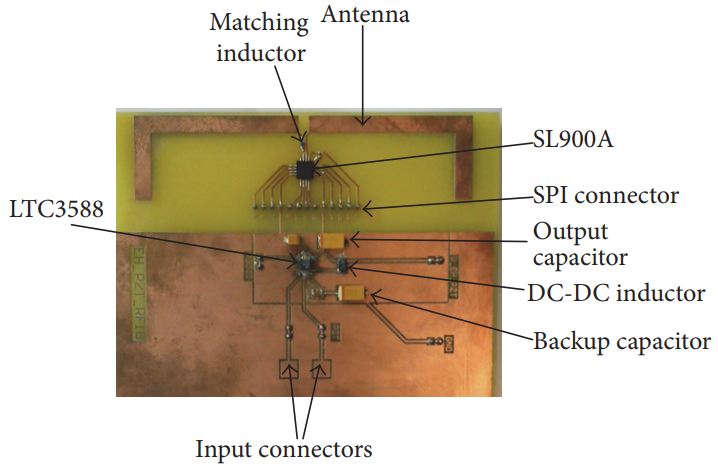
\includegraphics[width=0.9\linewidth]{../assets/viva/passive_tag_prototype.png}
				}
				\label{fi:passive_tag_prototype}
			}\\
			\subfloat[Equivalent Circuit]{
				\resizebox{0.7\linewidth}{!}{
					\begin{circuitikz}[transform shape]
	\tikzstyle{every node}=[font=\Large]
	\draw (0,0) coordinate(O)
	to [sV,l=$V_0$] ++(0,1.5)
	to [L,l=$X_{\text{A}}$] ++(0,1.5)
	to [R=$R_{\text{A}}$,-*] ++(3,0) coordinate(AM)
	to [sI,l_=$I_0$,-*] ++(0,-3)
	to [short] (O);
	\draw (AM)
	to [short] ++(0.5,0)
	to [L,l=$X_m$,-*] ++(3,0) coordinate(M)
	to [R=$R_{\text{S},m}$] ++(3,0) coordinate(MH);
	\draw (M)
	to [R=$R_{\text{P},m}$,-*] ++(0,-3);
	\draw (MH)
	to [D,-*] ++(1.5,0) coordinate(H)
	to [C=$X_{\text{H}}$,-*] ++(0,-3);
	\draw (H)
	to [short] ++(1.5,0)
	to [R=$R_{\text{H}}$] ++(0,-3)
	to [short] (O);

	\draw [dashed] (-1.125,-0.5) rectangle (3.5,4);
	\draw [dashed] (4,-0.5) rectangle (9,4);
	\draw [dashed] (9.5,-0.5) rectangle (13.5,4);

	\draw (1.125,4.25) node[]{Antenna};
	\draw (6.5,4.25) node[]{Modulator};
	\draw (11.5,4.25) node[]{Harvester \& Chip};

	\draw (3.375,2.675) to [short] (3.375,3.175) to [short] (3.25,3.175) to [short,i_=$Z_{\text{A}}$] (3.125,3.175);
	\draw (4.125,-0.125) to [short] (4.125,0.375) to [short] (4.25,0.375) to [short,i=$Z_m$] (4.375,0.375);
	\draw (9.625,-0.125) to [short] (9.625,0.375) to [short] (9.75,0.375) to [short,i=$Z_{\text{H}}$] (9.875,0.375);
\end{circuitikz}

				}
				\label{fg:equivalent_circuit}
			}
		\end{figure}
		Impinging waves can be used for powering, modulation, \textcolor{blue}{and beamforming.}
	\end{frame}

	\begin{frame}{Reflection coefficient}
		The node changes state by switching load impedance (and reflection coefficient)
		\begin{equation*}
			\Gamma = \frac{Z_\mathrm{L} - Z_0^*}{Z_\mathrm{L} + Z_0}
		\end{equation*}
		\vspace{-0.25cm}
		\begin{figure}
			\centering
			\resizebox{0.6\columnwidth}{!}{
				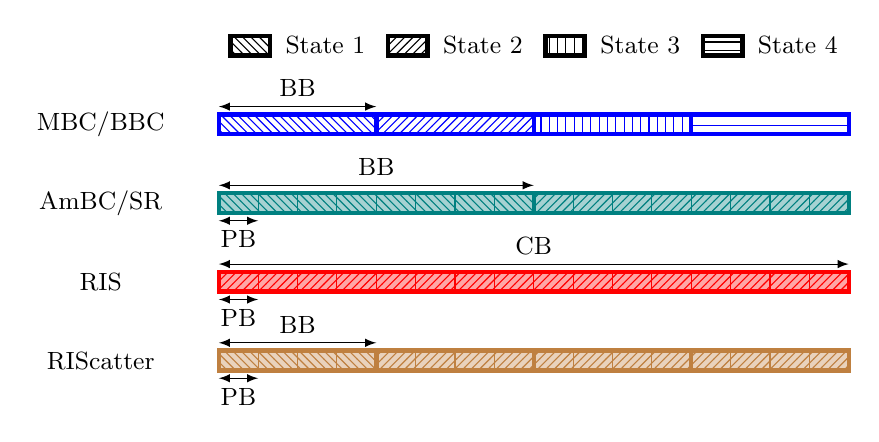
\begin{tikzpicture}[font=\small]
	% MBC/BBC
	\foreach \x in {0}{
			\draw[blue,ultra thick,postaction={pattern=north west lines},pattern color=.] (2*\x,4) rectangle ++(2,0.25);
		}
	\foreach \x in {1}{
			\draw[blue,ultra thick,postaction={pattern=north east lines},pattern color=.] (2*\x,4) rectangle ++(2,0.25);
		}
	\foreach \x in {2}{
			\draw[blue,ultra thick,postaction={pattern=vertical lines},pattern color=.] (2*\x,4) rectangle ++(2,0.25);
		}
	\foreach \x in {3}{
			\draw[blue,ultra thick,postaction={pattern=horizontal lines},pattern color=.] (2*\x,4) rectangle ++(2,0.25);
		}
	\draw[latex-latex] (0,4.35) -- (2,4.35) node[above,midway]{BB};
	\node at (-1.5,4.125) {MBC/BBC};

	% AmBC/SR
	\foreach \x in {0,...,7}{
			\draw[teal,fill=teal!35!white,postaction={pattern=north west lines},pattern color=.] (0.5*\x,3) rectangle ++(0.5,0.25);
		}
	\foreach \x in {8,...,15}{
			\draw[teal,fill=teal!35!white,postaction={pattern=north east lines},pattern color=.] (0.5*\x,3) rectangle ++(0.5,0.25);
		}
	\foreach \x in {0,...,1}{
			\draw[teal,ultra thick] (4*\x,3) rectangle ++(4,0.25);
		}
	\draw[latex-latex] (0,3.35) -- (4,3.35) node[above,midway]{BB};
	\draw[latex-latex] (0,2.9) -- (0.5,2.9) node[below,midway]{PB};
	\node at (-1.5,3.125) {AmBC/SR};

	% RIS
	\foreach \x in {0,...,15}{
			\draw[red,fill=red!35!white,postaction={pattern=north east lines},pattern color=.] (0.5*\x,2) rectangle ++(0.5,0.25);
		}
	\draw[red,ultra thick] (0,2) rectangle ++(8,0.25);
	\draw[latex-latex] (0,2.35) -- (8,2.35) node[above,midway]{CB};
	\draw[latex-latex] (0,1.9) -- (0.5,1.9) node[below,midway]{PB};
	\node at (-1.5,2.125) {RIS};

	% RIScatter
	\foreach \x in {0,...,3}{
			\draw[brown,fill=brown!35!white,postaction={pattern=north west lines},pattern color=.] (0.5*\x,1) rectangle ++(0.5,0.25);
		}
	\foreach \x in {4,...,15}{
			\draw[brown,fill=brown!35!white,postaction={pattern=north east lines},pattern color=.] (0.5*\x,1) rectangle ++(0.5,0.25);
		}
	\foreach \x in {0,...,3}{
			\draw[brown,ultra thick] (2*\x,1) rectangle ++(2,0.25);
		}
	\draw[latex-latex] (0,1.35) -- (2,1.35) node[above,midway]{BB};
	\draw[latex-latex] (0,0.9) -- (0.5,0.9) node[below,midway]{PB};

	\node at (-1.5,1.125) {RIScatter};

	\draw [pattern=north west lines,ultra thick](0.15,5) rectangle ++(0.5,0.25) node[xshift=20,yshift=-3.5] {State 1};
	\draw [pattern=north east lines,ultra thick](2.15,5) rectangle ++(0.5,0.25) node[xshift=20,yshift=-3.5] {State 2};
	\draw [pattern=vertical lines,ultra thick](4.15,5) rectangle ++(0.5,0.25) node[xshift=20,yshift=-3.5] {State 3};
	\draw [pattern=horizontal lines,ultra thick](6.15,5) rectangle ++(0.5,0.25) node[xshift=20,yshift=-3.5] {State 4};
\end{tikzpicture}

			}
		\end{figure}
		\vspace{-0.25cm}
		\begin{itemize}
			\item \gls{ris}: the state at a specific time is known (as a passive beamforming codeword) to the transceiver
			\begin{equation*}
				\Gamma_m = \exp(j \phi_m),
			\end{equation*}
			\item \gls{bc}: all states occur with equal probability (as part of information codeword) to be detected at the receiver
			\begin{equation*}
				\Gamma_m = \alpha_m \frac{c_m}{\max_{m'} \lvert c_{m'} \rvert},
			\end{equation*}
		\end{itemize}
	\end{frame}

	\begin{frame}{RIScatter system}
		\begin{table}
			\rowcolors{2}{gray!25}{white}
			\renewcommand{\arraystretch}{1.25}
			\resizebox{\linewidth}{!}{
				\begin{tabular}{c c c c c c}
					\toprule
					\hiderowcolors
					                       & Backscatter        & Ambient backscatter         & Symbiotic radio          & \gls{ris}           & RIScatter                        \\ \midrule
					\showrowcolors
					Information link(s)    & Backscatter        & Coexisting                  & Coexisting               & Primary             & Coexisting                       \\
					Primary on backscatter & Carrier            & Multiplicative interference & Spreading code           & ---                 & Energy uncertainty               \\
					Backscatter on primary & ---                & Multiplicative interference & Channel uncertainty      & Passive beamforming & Dynamic passive beamforming      \\
					Cooperative devices    & ---                & No                          & Transmitter and receiver & ---                 & Transmitter, nodes, and receiver \\
					Sequential decoding    & ---                & No                          & Primary-to-backscatter   & ---                 & Backscatter-to-primary           \\
					Reflection pattern by  & Information source & Information source          & Information source       & Channel             & Source, channel, and priority    \\
					Input distribution     & Equiprobable       & Equiprobable                & Equiprobable or Gaussian & Degenerate          & Flexible                         \\
					Load-switching speed   & Fast               & Slow                        & Slow                     & Quasi-static        & Arbitrary                        \\ \bottomrule
				\end{tabular}
			}
		\end{table}
		\begin{columns}
			\begin{column}{0.4\textwidth}
				\begin{figure}
					\centering
					\resizebox{\linewidth}{!}{
						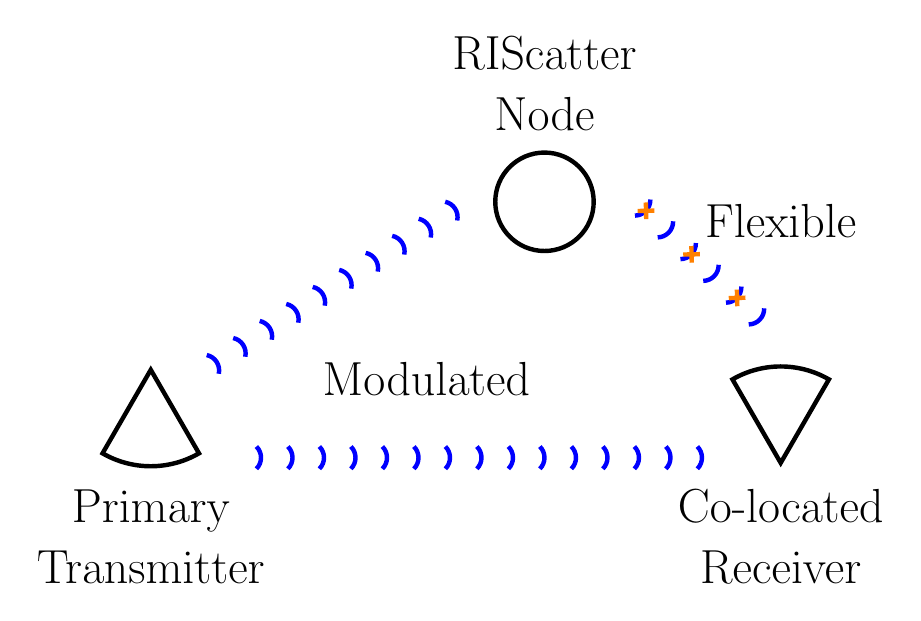
\begin{tikzpicture}[font=\LARGE,every node/.style={draw,ultra thick},every path/.style={ultra thick},every text node part/.style={align=center}]
	\node at (0,0) [circular sector,shape border rotate=90,minimum width=2cm] {};
	\node at (5,3) [circle,minimum size=1.25cm] {};
	\node at (8,0.55) [circular sector,shape border rotate=270,minimum width=2cm] {};

	\node[draw=none] at (0,-1.25) {Primary\\Transmitter};
	\node[draw=none] at (5,4.5) {RIScatter\\Node};
	\node[draw=none] at (8,-1.25) {Co-located\\Receiver};

	\draw[blue,decorate,decoration={waves,segment length=4mm,radius=2mm}] (1,-0.25) -- (7.375,-0.25);
	\draw[blue,decorate,decoration={waves,segment length=4mm,radius=2mm}] (0.5,0.75) -- (4,3);
	\draw[blue,decorate,decoration={waves,segment length=4mm,radius=2mm}] (6,3.1625) -- (8,1.25);
	\draw[orange,decorate,decoration={crosses,segment length=8mm,shape size=1.5mm}] (6.29,2.885) -- (8,1.25);

	\node[draw=none] at (3.5,0.75) {Modulated};
	\node[draw=none] at (8,2.76) {Flexible};
\end{tikzpicture}

					}
					\label{fg:riscatter}
				\end{figure}
			\end{column}
			\begin{column}{0.5\textwidth}
				\begin{itemize}
						\item {\color{blue}Primary link:} active legacy transmission from an \gls{rf} source
						\item {\color{orange}Backscatter link:} passive free-ride transmission from RIScatter nodes
				\end{itemize}
			\end{column}
		\end{columns}
		RIScatter renders the node input distribution as a function of information source, \gls{csi}, and priority of coexisting links.
	\end{frame}

	\begin{frame}{Signal model}
		\begin{figure}[H]
			\centering
			\def\svgwidth{0.6\columnwidth}
			\input{../assets/viva/riscatter_network.pdf_tex}
			\label{fg:riscatter_network}
		\end{figure}
		Within each backscatter block, received signal at primary block $n$ is
		\begin{equation*}
			y[n] = \underbrace{\Bigl(\mathbf{h}_{\text{D}}^\mathsf{H} + \sum_{k} \alpha_k \mathbf{h}_{\text{C},k}^\mathsf{H} \textcolor{orange}{x_k}\Bigr)}_{\mathbf{h}^\mathsf{H}(\textcolor{orange}{x_{\mathcal{K}}})} \mathbf{w} \textcolor{blue}{s[n]} + v[n],
		\end{equation*}
		\vspace{-0.25cm}
		\begin{block}{Properties}
			\begin{enumerate}
				\item \textcolor{blue}{Primary} and \textcolor{orange}{backscatter} symbols are superimposed by {double modulation}
				\item Backscatter signal is much weaker due to {double fading}
				\item The spreading factor (i.e., symbol period ratio $N$) is usually large
				\item Each {state} is simultaneously part of information and beamforming {codeword}
				\item Reflection pattern over time is guided by input probability distribution
			\end{enumerate}
		\end{block}
	\end{frame}

	\begin{frame}{Low-complexity receiver}
		We propose a low-complexity receiver that exploits the aforementioned properties to avoid \gls{sic}.
		\begin{figure}[!t]
			\centering
			\subfloat{
				\resizebox{0.42\linewidth}{!}{
					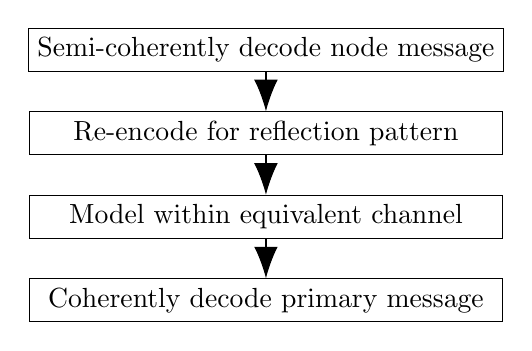
\begin{tikzpicture}[
		% every axis plot/.append style={thick},
		every node/.append style={draw,minimum width=6cm},
		align=center
	]
	\draw[-{Latex[length=4mm]}] (0,0) node[anchor=south](0){Semi-coherently decode node message} to ++(0,-0.5) node[anchor=north](1){Re-encode for reflection pattern};
	\draw[-{Latex[length=4mm]}] (1.south) to ++(0,-0.5) node[anchor=north](2){Model within equivalent channel};
	\draw[-{Latex[length=4mm]}] (2.south) to ++(0,-0.5) node[anchor=north](3){Coherently decode primary message};
\end{tikzpicture}

				}
			}
			\subfloat{
				\resizebox{0.58\linewidth}{!}{
					\definecolor{color1}{HTML}{0072BD}
\definecolor{color2}{HTML}{D95319}
\definecolor{color3}{HTML}{EDB120}
\definecolor{color4}{HTML}{7E2F8E}

\begin{tikzpicture}
	\begin{axis}[
			clip mode=individual,
			height=4cm,
			width=10cm,
			xlabel = $z$,
			ylabel = {Probability Density},
			font=\normalsize,
			no markers,
			xmin=0,
			ymin=0,
			xmax=70,
			xtick={0,12.78,20.28,29.62,70},
			xticklabels={$t_0$,$t_1$,$t_2$,$t_3$,$t_4$},
			yticklabels=\empty,
			samples = 200
		]

		\addplot+[very thick,solid,color1] gnuplot[raw gnuplot,smooth] {%
				isint(x) = (int(x)==x);
				gmm(x,rho,lambda)=rho<=0||lambda<=0?1/0:  x<0?0.0:x==0?(rho>1?0.0:rho==1?real(lambda):1/0):  exp(rho*log(lambda)+(rho-1.0)*log(x)-lgamma(rho)-lambda*x);
				set xrange [0:80];
				set yrange [0:1];
				samples=200;
				plot gmm(x,10,1)};
		\addlegendentryexpanded{$f(z \mid x_1)$}

		\addplot+[very thick,dashed,color2] gnuplot[raw gnuplot,smooth] {%
				isint(x) = (int(x)==x);
				gmm(x,rho,lambda)=rho<=0||lambda<=0?1/0:  x<0?0.0:x==0?(rho>1?0.0:rho==1?real(lambda):1/0):  exp(rho*log(lambda)+(rho-1.0)*log(x)-lgamma(rho)-lambda*x);
				set xrange [0:80];
				set yrange [0:1];
				samples=200;
				plot gmm(x,10,0.6)};
		\addlegendentryexpanded{$f(z \mid x_2)$}

		\addplot+[very thick,dotted,color3] gnuplot[raw gnuplot,smooth] {%
				isint(x) = (int(x)==x);
				gmm(x,rho,lambda)=rho<=0||lambda<=0?1/0:  x<0?0.0:x==0?(rho>1?0.0:rho==1?real(lambda):1/0):  exp(rho*log(lambda)+(rho-1.0)*log(x)-lgamma(rho)-lambda*x);
				set xrange [0:80];
				set yrange [0:1];
				samples=200;
				plot gmm(x,10,0.4)};
		\addlegendentryexpanded{$f(z \mid x_3)$}

		\addplot+[very thick,dashdotted,color4] gnuplot[raw gnuplot,smooth] {%
				isint(x) = (int(x)==x);
				gmm(x,rho,lambda)=rho<=0||lambda<=0?1/0:  x<0?0.0:x==0?(rho>1?0.0:rho==1?real(lambda):1/0):  exp(rho*log(lambda)+(rho-1.0)*log(x)-lgamma(rho)-lambda*x);
				set xrange [0:80];
				set yrange [0:1];
				samples=200;
				plot gmm(x,10,0.28)};
		\addlegendentryexpanded{$f(z \mid x_4)$}
		\draw[latex-latex] (0,0) -- (12.78,0) node[above,midway,yshift=-2]{$\mathcal{R}_1$};
		\draw[latex-latex] (12.78,0) -- (20.28,0) node[above,midway,yshift=-2]{$\mathcal{R}_2$};
		\draw[latex-latex] (20.28,0) -- (29.62,0) node[above,midway,yshift=-2]{$\mathcal{R}_3$};
		\draw[latex-latex] (29.62,0) -- (70,0) node[above,midway,yshift=-2]{$\mathcal{R}_4$};
	\end{axis}
\end{tikzpicture}

				}
			}
			\label{fg:receiver}
		\end{figure}
		\vspace{0.5cm}
		\begin{itemize}
			\item Accumulated receive energy $z=\sum_{n} \bigl\lvert y[n] \bigr\rvert^2$ follows Gamma distribution
			\item \textcolor{orange}{Backscatter detection} under primary uncertainty is part of \textcolor{blue}{channel training}
			\item Requires one energy comparison and re-encoding per backscatter symbol (much simpler than symbiotic radio with $N$ \gls{sic} and 1 combining)
		\end{itemize}
	\end{frame}


	\begin{frame}{Joint beamforming, input distribution, and energy detector design}
		\vspace{-0.125cm}
		\begin{block}{Achievable rate}
			\vspace{-0.25cm}
			\begin{align*}
				\sum_k R_{\text{B},k} &= \sum\nolimits_{m_{\mathcal{K}}} P_{\mathcal{K}}(x_{m_{\mathcal{K}}}) \sum\nolimits_{m_{\mathcal{K}}'} P(\hat{x}_{m_{\mathcal{K}}'} \mid x_{m_{\mathcal{K}}}) \log {P(\hat{x}_{m_{\mathcal{K}}'} \mid x_{m_{\mathcal{K}}})}/{P(\hat{x}_{m_{\mathcal{K}}'})}\\
				R_{\text{P}} &= \sum\nolimits_{m_{\mathcal{K}}} P_{\mathcal{K}}(x_{m_{\mathcal{K}}}) N \log \left(1 + \frac{\lvert \mathbf{h}^\mathsf{H}(x_{m_{\mathcal{K}}}) \mathbf{w} \rvert^2}{\sigma_w^2}\right)
			\end{align*}
		\end{block}
		\begin{block}{Problem formulation}
			\vspace{-0.25cm}
			\begin{maxi*}
				{\scriptstyle{\{\mathbf{p}_k\},\mathbf{w},\mathbf{t}}}{\rho R_\text{P} + (1-\rho) \sum\nolimits_{k} R_{\text{B},k}}{}{}
				\addConstraint{\mathbf{1}^\mathsf{T} \mathbf{p}_k=1,}{\quad \mathbf{p}_k \ge \mathbf{0},}{\quad \forall k}
				\addConstraint{t_{l-1} \le t_l,}{\quad t_l \ge 0,}{\quad \forall l}
				\addConstraint{\lVert \mathbf{w} \rVert^2 \le P,}{}{}
			\end{maxi*}
		\end{block}
		\begin{exampleblock}{Solution by \gls{bcd}}
			\begin{itemize}
				\item Input distribution $\{\mathbf{p}_k\}$: \gls{kkt}
				\item Active beamforming $\mathbf{w}$: \gls{pga}
				\item Energy decision threshold $\mathbf{t}$: \gls{dp}
			\end{itemize}
		\end{exampleblock}
	\end{frame}

	\begin{frame}{Simulation results: Input distribution}
		\begin{figure}[!t]
			\centering
			\subfloat{
				\resizebox{0.48\linewidth}{!}{
					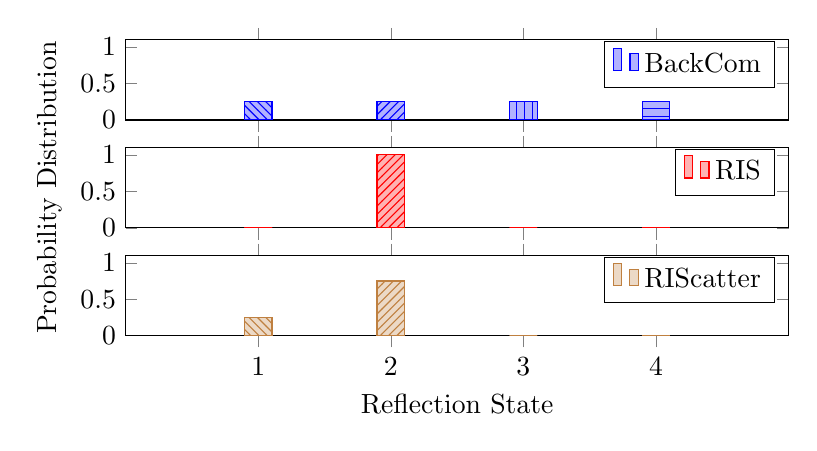
\begin{tikzpicture}
	\begin{groupplot}
		[group style={
					rows=3,
					group name=plots,
					x descriptions at=edge bottom,
					y descriptions at=edge left,
					vertical sep=10
				},
			ybar,
			xmin=0,
			xmax=4,
			xtick={1,2,3,4},
			ymin=0,
			ymax=1,
			xlabel={Reflection State},
			enlarge x limits={value=0.25,upper},
			enlarge y limits={value=0.1,upper},
			width=10cm,
			height=2.6cm,
			every axis plot/.append style={bar shift=0}
		]
		\nextgroupplot
		\addplot[blue,fill=blue!30!white] coordinates {(-1,-1)};
		\addplot[blue,fill=blue!30!white,postaction={pattern=north west lines},pattern color=.] coordinates {(1,0.25)};
		\addplot[blue,fill=blue!30!white,postaction={pattern=north east lines},pattern color=.] coordinates {(2,0.25)};
		\addplot[blue,fill=blue!30!white,postaction={pattern=vertical lines},pattern color=.] coordinates {(3,0.25)};
		\addplot[blue,fill=blue!30!white,postaction={pattern=horizontal lines},pattern color=.] coordinates {(4,0.25)};
		\legend{BackCom}
		\nextgroupplot[ylabel={Probability Distribution}]
		\addplot[red,fill=red!30!white] coordinates {(-1,-1)};
		\addplot[red,fill=red!30!white,postaction={pattern=north west lines},pattern color=.] coordinates {(1,0)};
		\addplot[red,fill=red!30!white,postaction={pattern=north east lines},pattern color=.] coordinates {(2,1)};
		\addplot[red,fill=red!30!white,postaction={pattern=vertical lines},pattern color=.] coordinates {(3,0)};
		\addplot[red,fill=red!30!white,postaction={pattern=horizontal lines},pattern color=.] coordinates {(4,0)};
		\legend{RIS}
		\nextgroupplot
		\addplot[brown,fill=brown!30!white] coordinates {(-1,-1)};
		\addplot[brown,fill=brown!30!white,postaction={pattern=north west lines},pattern color=.] coordinates {(1,0.25)};
		\addplot[brown,fill=brown!30!white,postaction={pattern=north east lines},pattern color=.] coordinates {(2,0.75)};
		\addplot[brown,fill=brown!30!white,postaction={pattern=vertical lines},pattern color=.] coordinates {(3,0)};
		\addplot[brown,fill=brown!30!white,postaction={pattern=horizontal lines},pattern color=.] coordinates {(4,0)};
		\legend{RIScatter}
	\end{groupplot}
\end{tikzpicture}

				}
			}
			\subfloat{
				\resizebox{0.48\linewidth}{!}{
					% This file was created by matlab2tikz.
%
%The latest updates can be retrieved from
%  http://www.mathworks.com/matlabcentral/fileexchange/22022-matlab2tikz-matlab2tikz
%where you can also make suggestions and rate matlab2tikz.
%
\definecolor{mycolor1}{rgb}{0.00000,0.44706,0.74118}%
\definecolor{mycolor2}{rgb}{0.85098,0.32549,0.09804}%
\definecolor{mycolor3}{rgb}{0.92941,0.69412,0.12549}%
\definecolor{mycolor4}{rgb}{0.49412,0.18431,0.55686}%
%
\begin{tikzpicture}

\begin{axis}[%
width=4.079in,
height=1.587in,
at={(0.684in,0.361in)},
scale only axis,
xmin=1,
xmax=4,
xtick={1, 2, 3, 4},
xlabel style={font=\color{white!15!black}},
xlabel={Reflection State},
ymin=0,
ymax=1,
ytick={  0, 0.2, 0.4, 0.6, 0.8,   1},
ylabel style={font=\color{white!15!black}},
ylabel={Probability\\Distribution},
axis background/.style={fill=white},
xmajorgrids,
ymajorgrids,
legend style={at={(0.03,0.97)}, anchor=north west, legend cell align=left, align=left, draw=white!15!black},
align=center,
title style={font=\LARGE},
label style={font=\LARGE},
ticklabel style={font=\Large},
legend style={font=\Large}
]
\addplot [color=mycolor1, line width=2.0pt, mark=o, mark options={solid, mycolor1}]
  table[row sep=crcr]{%
1	6.48337921881147e-07\\
2	0.504332536970115\\
3	0.495666065268481\\
4	7.49423481629768e-07\\
};
\addlegendentry{$\rho =0$}

\addplot [color=mycolor2, dashed, line width=2.0pt, mark=+, mark options={solid, mycolor2}]
  table[row sep=crcr]{%
1	9.07520883479571e-08\\
2	0.401497967775065\\
3	0.598501822229458\\
4	1.1924338950349e-07\\
};
\addlegendentry{$\rho =0.1$}

\addplot [color=mycolor3, dotted, line width=2.0pt, mark=square, mark options={solid, mycolor3}]
  table[row sep=crcr]{%
1	5.20790909800095e-09\\
2	0.192484685585801\\
3	0.807515300031504\\
4	9.17478600370393e-09\\
};
\addlegendentry{$\rho =0.25$}

\addplot [color=mycolor4, dashdotted, line width=2.0pt, mark=x, mark options={solid, mycolor4}]
  table[row sep=crcr]{%
1	1.08446044988811e-11\\
2	8.27854203489531e-06\\
3	0.999991721175464\\
4	2.71656646770891e-10\\
};
\addlegendentry{$\rho =1$}

\end{axis}
\end{tikzpicture}%
				}
			}
		\end{figure}
		\begin{itemize}
			\item \gls{bc} and \gls{ris} are special cases of RIScatter with uniform and degenerate input distribution
			\item Increasing $\rho$ from 0 to 1 creates a smooth transition from backscatter modulation to passive beamforming
		\end{itemize}
	\end{frame}

	\begin{frame}{Simulation results: Rate region}
		\begin{figure}[!t]
			\centering
			\subfloat{
				\resizebox{0.48\linewidth}{!}{
					% This file was created by matlab2tikz.
%
%The latest updates can be retrieved from
%  http://www.mathworks.com/matlabcentral/fileexchange/22022-matlab2tikz-matlab2tikz
%where you can also make suggestions and rate matlab2tikz.
%
\definecolor{mycolor1}{rgb}{0.30100,0.74500,0.93300}%
\definecolor{mycolor2}{rgb}{0.46600,0.67400,0.18800}%
\definecolor{mycolor3}{rgb}{0.49400,0.18400,0.55600}%
\definecolor{mycolor4}{rgb}{0.92900,0.69400,0.12500}%
\definecolor{mycolor5}{rgb}{0.85000,0.32500,0.09800}%
\definecolor{mycolor6}{rgb}{0.00000,0.44700,0.74100}%
%
\begin{tikzpicture}

\begin{axis}[%
	width=4.079in,
	height=3.432in,
at={(0.673in,0.356in)},
scale only axis,
xmin=0,
xmax=6.5227548374066,
xlabel style={font=\color{white!15!black}},
xlabel={Primary Rate [bits/s/Hz]},
ymin=0,
ymax=2,
ylabel style={font=\color{white!15!black}},
ylabel={Backscatter Rate [bits/BB]},
axis background/.style={fill=white},
xmajorgrids,
ymajorgrids,
legend style={at={(0.03,0.97)}, anchor=north west, legend cell align=left, align=left, draw=white!15!black},
align=center,
% title style={font=\huge},
% label style={font=\huge},
% ticklabel style={font=\LARGE},
% legend style={font=\LARGE},
reverse legend,
every axis plot/.append style={line width=2pt}
]
\addplot [color=mycolor1, line width=2.0pt, mark=triangle, mark options={solid, rotate=180, mycolor1}]
  table[row sep=crcr]{%
6.33724402501803	1.39764296268229\\
0	1.39764296268229\\
0	0\\
6.52275483678685	0\\
6.52275483678685	2.37312052924553e-08\\
6.38739454470992	1.3235811846854\\
6.35422040211439	1.38916612409166\\
6.34857862205488	1.39386686170527\\
6.3445353675389	1.39608085009443\\
6.34291602910554	1.3966977322109\\
6.34149846039129	1.39711118534274\\
6.34024731759122	1.39737797077851\\
6.3391350240222	1.3975379071887\\
6.33862394227692	1.39758701988787\\
6.33813974610465	1.39761939115801\\
6.33795313341839	1.39762818964178\\
6.33777036860279	1.39763482338317\\
6.3375913342378	1.3976394187338\\
6.33741590881855	1.39764209463684\\
6.33724402501803	1.39764296268229\\
};
\addlegendentry{RIScatter}

\addplot[only marks, mark=triangle, mark options={}, mark size=2.3570pt, draw=mycolor2] table[row sep=crcr]{%
x	y\\
6.5227548374066	0\\
};
\addlegendentry{RIS}

\addplot[only marks, mark=+, mark options={}, mark size=3.5355pt, draw=mycolor3] table[row sep=crcr]{%
x	y\\
6.34321982467796	2\\
};
\addlegendentry{SR}

\addplot[only marks, mark=x, mark options={}, mark size=3.5355pt, draw=mycolor4] table[row sep=crcr]{%
x	y\\
5.90778796357092	1.34857377961699\\
};
\addlegendentry{AmBC}

\addplot[only marks, mark=square, mark options={}, mark size=2.5000pt, draw=mycolor5] table[row sep=crcr]{%
x	y\\
0	1.99999999999997\\
};
\addlegendentry{BBC}

\addplot[only marks, mark=o, mark options={}, mark size=2.7386pt, draw=mycolor6] table[row sep=crcr]{%
x	y\\
6.34314881160129	0\\
};
\addlegendentry{Legacy}

\end{axis}
\end{tikzpicture}%

				}
			}
			\subfloat{
				\resizebox{0.48\linewidth}{!}{
					% This file was created by matlab2tikz.
%
%The latest updates can be retrieved from
%  http://www.mathworks.com/matlabcentral/fileexchange/22022-matlab2tikz-matlab2tikz
%where you can also make suggestions and rate matlab2tikz.
%
\definecolor{mycolor1}{rgb}{0.00000,0.44706,0.74118}%
\definecolor{mycolor2}{rgb}{0.85098,0.32549,0.09804}%
\definecolor{mycolor3}{rgb}{0.92941,0.69412,0.12549}%
\definecolor{mycolor4}{rgb}{0.49412,0.18431,0.55686}%
%
\begin{tikzpicture}

\begin{axis}[%
width=4.079in,
height=3.432in,
at={(0.684in,0.463in)},
scale only axis,
xmin=0,
xmax=8.8183272162648,
xlabel style={font=\color{white!15!black}},
xlabel={Primary Rate [bits/s/Hz]},
ymin=0,
ymax=0.0387033207318202,
ylabel style={font=\color{white!15!black}},
ylabel={Total Backscatter Rate [bits/PB]},
axis background/.style={fill=white},
xmajorgrids,
ymajorgrids,
legend style={legend cell align=left, align=left, draw=white!15!black},
% title style={font=\huge},
% label style={font=\huge},
% ticklabel style={font=\LARGE},
% legend style={font=\LARGE},
scaled y ticks=false,
y tick label style={/pgf/number format/.cd, fixed, precision=3}
]
\addplot [color=mycolor1, line width=2.0pt, mark=o, mark options={solid, mycolor1}]
  table[row sep=crcr]{%
1.48510320561817	0.0368420449632478\\
0	0.0368420449632478\\
0	0\\
8.81494977830283	0\\
8.81494977830283	3.83377782240587e-09\\
8.81477352076949	4.12086540411783e-05\\
8.80464308481592	0.00150570482545958\\
8.79481987635483	0.00225430896534762\\
8.77713969997226	0.00314972206304367\\
8.76137548769293	0.00370957602960849\\
8.73671299086267	0.00438218933776903\\
8.69453600558026	0.00520601203273033\\
8.28548800580697	0.0100384418588948\\
7.50094640226552	0.0164759402145025\\
6.17365035431449	0.0243306497651073\\
5.38460240649074	0.0281228393432611\\
4.43736577109357	0.0316815244629786\\
3.35788745554615	0.0347239772599961\\
2.42247216478758	0.0363829293680192\\
1.48510320561817	0.0368420449632478\\
};
\addlegendentry{$N =10$}

\addplot [color=mycolor2, dashed, line width=2.0pt, mark=+, mark options={solid, mycolor2}]
  table[row sep=crcr]{%
1.67326087069726	0.0387033207318202\\
0	0.0387033207318202\\
0	0\\
8.81632618502012	0\\
8.81632618502012	3.78776722621619e-09\\
8.81475527355384	0.000280915977176361\\
8.79137070993339	0.00206604004006254\\
8.77128743184392	0.00286700361188652\\
8.73376638330174	0.00384928202287025\\
8.70398959350056	0.00439622330702994\\
8.65744036384737	0.00503258656132342\\
8.09711868907005	0.00979758641066475\\
5.99563108181371	0.0228762637504772\\
4.45257316761243	0.0300452011722592\\
2.27166407033345	0.0382673640700557\\
2.16776341617934	0.0385860807078977\\
1.67326087069726	0.0387033207318202\\
};
\addlegendentry{$N =20$}

\addplot [color=mycolor3, dotted, line width=2.0pt, mark=square, mark options={solid, mycolor3}]
  table[row sep=crcr]{%
1.83746579456681	0.0276333556833912\\
0	0.0276333556833912\\
0	0\\
8.81770456115495	0\\
8.81770456115495	3.7090329843289e-09\\
8.81076099034007	0.000692022846241925\\
8.76252321046823	0.0026134586736102\\
8.72405262673134	0.00338528337241505\\
8.66910163543863	0.00412499790973992\\
8.63636424982091	0.00443320983809654\\
8.49104009736616	0.00532943743607748\\
6.632727264277	0.0136498550235196\\
3.97653834627339	0.022619911417612\\
2.52017820134887	0.0269919450432153\\
2.36966502343278	0.0273353671781562\\
2.26462330968326	0.0274987365111921\\
1.83746579456681	0.0276333556833912\\
};
\addlegendentry{$N =40$}

\addplot [color=mycolor4, dashdotted, line width=2.0pt, mark=x, mark options={solid, mycolor4}]
  table[row sep=crcr]{%
1.92697586132023	0.0156929341853527\\
0	0.0156929341853527\\
0	0\\
8.8183272162648	0\\
8.8183272162648	3.59260549629013e-09\\
8.79705312747263	0.0011834340984776\\
8.71449510548813	0.00289050386525025\\
8.6694989698604	0.00334507596844779\\
8.61820727629173	0.00370001890167476\\
8.58563007809167	0.00385293178365339\\
8.07998156196288	0.00534682829297022\\
5.73983931093962	0.0105561822763253\\
4.02882077928576	0.0135099872091105\\
3.51115343811173	0.0143127975860811\\
3.14578535673428	0.0148283101617506\\
2.91655857645647	0.0151149267525588\\
2.72534244455508	0.0153412126648229\\
2.51360524723683	0.0155222047472113\\
2.33087009972618	0.0156260932199399\\
1.92697586132023	0.0156929341853527\\
};
\addlegendentry{$N =80$}

\end{axis}
\end{tikzpicture}%

				}
			}
		\end{figure}
		\begin{itemize}
			\item RIScatter backscatter rate is lower than symbiotic radio (due to energy detection) but higher than ambient backscatter (due to adaptive encoding)
			\item A large spreading factor $N$ improves backscatter \glsfmtshort{ber} but reduces data rate
			\item Active and passive transmission can share resource with mutual benefits
		\end{itemize}
	\end{frame}
\end{section}

\begin{section}{Shaping: \glsfmtshort{bd}-\glsfmtshort{ris} in \glsfmtshort{mimo}}
	\begin{frame}{Channel shaping using \glsfmtshort{ris}: From diagonal model to beyond}
		\begin{block}{Overview}
			\begin{itemize}\setlength\itemsep{20pt}
				\item \textit{What does this paper study?}

				To what extent can a passive \gls{ris} redistribute the singular values of a \gls{mimo} channel.
				\item \textit{How does it differ from previous work?}

				We consider a \gls{bd} architecture, depict the singular value region, derive analytical bounds, and solve the rate maximization problem.
				\item \textit{What are the benefits?}

				Channel shaping is ubiquitous for communication, sensing, and power transfer, which helps to decouple the \gls{ris}-transceiver design.
				We also propose an efficient and universal \gls{bd}-\gls{ris} design framework.
			\end{itemize}
		\end{block}
	\end{frame}

	\begin{frame}{Wave scattering model}
		\begin{block}{Diagonal \glsfmtshort{ris}}
			Each element acts as an individual scatterer with phase shift only
			\begin{equation*}
				\mathbf{\Theta} = \mathrm{diag}(\theta_1, \ldots, \theta_{N_\mathrm{S}}) = \mathrm{diag}(e^{\jmath \phi_1}, \ldots, e^{\jmath \phi_{N_\mathrm{S}}})
				%  =
				% \begin{bsmallmatrix}
				% 	\theta_1 & 0 & \cdots & 0 \\
				% 	0 & \theta_2 & \cdots & 0 \\
				% 	\vdots & \vdots & \ddots & \vdots \\
				% 	0 & 0 & \cdots & \theta_{N_\mathrm{S}}
				% \end{bsmallmatrix}
				\label{eq:diagonal_scattering_matrix}
			\end{equation*}
		\end{block}

		\begin{block}{\glsfmtshort{bd}-\glsfmtshort{ris}}
			Each group contains $L$ connected elements, allowing amplitude and phase control
			\vspace{-0.25cm}
			\begin{equation*}
				\mathbf{\Theta} = \mathrm{diag}(\mathbf{\Theta}_1,\ldots,\mathbf{\Theta}_G), \quad \mathbf{\Theta}_g^\mathsf{H} \mathbf{\Theta}_g = \mathbf{I}_L, \quad \forall g
				\label{eq:bd_ris}
			\end{equation*}
			\vspace{-0.5cm}
			\begin{itemize}
				\item \emph{Subchannel rearrangement:} allows each group to rearrange and combine the backward and forward subchannels by strength
				\vspace{-0.25cm}
				\begin{equation*}
					\sum_{n=1}^{N_\mathrm{S}} \lvert h_{\mathrm{B},n} \rvert \lvert h_{\mathrm{F},n} \rvert \to \sum_{g=1}^{G} \sum_{l=1}^{L} \lvert h_{\mathrm{B},\pi_{\mathrm{B},g}(l)} \rvert \lvert h_{\mathrm{F},\pi_{\mathrm{F},g}(l)} \rvert
					\vspace{-0.25cm}
				\end{equation*}
				\item \emph{Subspace alignment:} rotate backward-forward (intra-group, multiplicative) and direct-indirect (inter-group, additive) singular vectors
				\vspace{-0.25cm}
				\begin{equation*}
					\mathbf{H} = \overbrace{\mathbf{H}_\mathrm{D} + \sum_g \mathbf{U}_{\mathrm{B},g} \mathbf{\Sigma}_{\mathrm{B},g} \underbrace{\mathbf{V}_{\mathrm{B},g}^\mathsf{H} \mathbf{\Theta}_g \mathbf{U}_{\mathrm{F},g}}_\text{backward-forward} \mathbf{\Sigma}_{\mathrm{F},g} \mathbf{V}_{\mathrm{F},g}^\mathsf{H}}^\text{direct-indirect}
					\label{eq:channel_equivalent_svd}
				\end{equation*}
			\end{itemize}
		\end{block}
	\end{frame}

	\begin{frame}{Some concepts in differential geometry}
		The feasible domain of $\mathbf{\Theta}_g$ is a unitary Lie group $U(L)$ with Lie algebra $\mathfrak{u}(L)$.
		\vspace{0.25em}
		\begin{itemize}
			\item \emph{Geodesic:} shortest path between two points on a manifold
			\item \emph{Lie group:} a group that is also a differentiable manifold
			\item \emph{Lie algebra:} tangent space of Lie group at the identity element
			% \item \emph{Exponential map:} maps the Lie algebra to the Lie group
		\end{itemize}
		\begin{figure}
			\centering
			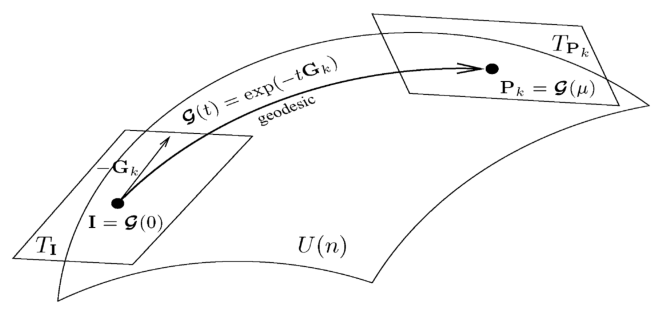
\includegraphics[width=0.65\textwidth]{../assets/viva/lie_group.pdf}
		\end{figure}
		A geodesic emanating from the identity with velocity $\mathbf{D} \in \mathfrak{u}(L)$ can be described by the exponential map
		\begin{equation*}
			\mathbf{G}_\mathbf{I}(\mu) = \exp(\mu \mathbf{D})
			\label{eq:geodesic_identity}
		\end{equation*}

	\end{frame}

	\begin{frame}{Geodesic \glsfmtshort{rcg} via Lie algebra}
		\begin{block}{Non-geodesic vs geodesic \gls{rcg}}
			\begin{itemize}
				\item Non-geodesic: add then retract
				\begin{equation*}
					\bar{\mathbf{\Theta}}_g^{(r+1)} = \mathbf{\Theta}_g^{(r)} + \mu \mathbf{D}_g^{(r)}, \quad \mathbf{\Theta}_g^{(r+1)} = \bar{\mathbf{\Theta}}_g^{(r+1)} \bigl({\bar{\mathbf{\Theta}}_g^{(r+1)\mathsf{H}}} \bar{\mathbf{\Theta}}_g^{(r+1)}\bigr)^{-1/2}
				\end{equation*}
				\item Geodesic: multiplicative and rotational update
				\begin{equation*}
					\mathbf{\Theta}_g^{(r+1)} = \mathbf{G}_g^{(r)}(\mu) = \exp(\mu \mathbf{D}_g^{(r)}) \mathbf{\Theta}_g^{(r)}
					\label{eq:update_geodesic}
				\end{equation*}
			\end{itemize}
		\end{block}
		\begin{exampleblock}{Performance comparison}
			\begin{table}
				\label{tb:complexity_test}
				\centering
				\tiny
				\begin{tabular}{ccccccc}
					\toprule
					\multirow{2}{*}{\gls{rcg} path} & \multicolumn{3}{c}{$N_\mathrm{S}=16$} & \multicolumn{3}{c}{$N_\mathrm{S}=256$}                                                               \\ \cmidrule(lr){2-4} \cmidrule(lr){5-7}
													& Objective                             & Iterations                             & Time [s]         & Objective        & Iterations & Time [s] \\ \midrule
					Geodesic                        & $\num{4.359e-3}$                      & 11.59                                  & $\num{1.839e-2}$ & $\num{1.163e-2}$ & 25.58      & 3.461    \\
					Non-geodesic                    & $\num{4.329e-3}$                      & 30.92                                  & $\num{5.743e-2}$ & $\num{1.116e-2}$ & 61.40      & 13.50    \\ \bottomrule
				\end{tabular}
			\end{table}
		\end{exampleblock}
	\end{frame}

	\begin{frame}{Singular value redistribution: Optimization approach}
		\begin{block}{Pareto frontier of singular values}
			\begin{maxi*}
				{\scriptstyle{\mathbf{\Theta}}}{\sum_n \rho_n \sigma_n(\mathbf{H})}{}{}
				\addConstraint{\mathbf{\Theta}_g^\mathsf{H} \mathbf{\Theta}_g=\mathbf{I},}{\quad \forall g,}{}
			\end{maxi*}
		\end{block}
		\begin{exampleblock}{Solution by group-wise geodesic \glsfmtshort{rcg}}
			\begin{itemize}
				\item Faster convergence thanks to appropriate parameter space
				\item Step size $\mu$ can be obtained by the Armijo rule
				\item Doubling $\mu$ is computationally efficient $\exp(2 \mu \mathbf{D}_g^{(r)}) = \exp^2(\mu \mathbf{D}_g^{(r)})$
			\end{itemize}
		\end{exampleblock}
	\end{frame}

	\begin{frame}{Singular value redistribution: Analysis approach}
		\fontsize{6pt}{7.2}\selectfont
		\begin{proposition}[Degree of freedom]\label{pp:dof}
			In point-to-point \gls{mimo}, \gls{bd}-\gls{ris} cannot achieve a higher \gls{dof} than diagonal \gls{ris}.
		\end{proposition}
		\begin{proposition}[Rank-deficient channel]\label{pp:rank_deficient}
			If the forward or backward channel is rank-$k$ ($k \le N$), then regardless of the passive \gls{ris} size and architecture, the $n$-th singular value of the equivalent channel is bounded by
			\begin{align*}
				\sigma_n(\mathbf{H}) & \le \sigma_{n-k}(\mathbf{T}), &  & \text{if } n > k,         \\
				\sigma_n(\mathbf{H}) & \ge \sigma_n(\mathbf{T}),     &  & \text{if } n < N - k + 1,
			\end{align*}
			where
			\begin{equation*}
				\mathbf{T} \mathbf{T}^\mathsf{H} =
				\begin{cases}
					\mathbf{H}_\mathrm{D} (\mathbf{I} - \mathbf{V}_\mathrm{F} \mathbf{V}_\mathrm{F}^\mathsf{H}) \mathbf{H}_\mathrm{D}^\mathsf{H}, & \text{if } \mathrm{rank}(\mathbf{H}_\mathrm{F}) = k, \\
					\mathbf{H}_\mathrm{D}^\mathsf{H} (\mathbf{I} - \mathbf{U}_\mathrm{B} \mathbf{U}_\mathrm{B}^\mathsf{H}) \mathbf{H}_\mathrm{D}, & \text{if } \mathrm{rank}(\mathbf{H}_\mathrm{B}) = k,
				\end{cases}
				\label{eq:auxiliary_matrix}
			\end{equation*}
			and $\mathbf{V}_\mathrm{F}$ and $\mathbf{U}_\mathrm{B}$ are the right and left compact singular matrices of $\mathbf{H}_\mathrm{F}$ and $\mathbf{H}_\mathrm{B}$, respectively.
		\end{proposition}
		\begin{proposition}[Unitary \gls{ris} without direct link]\label{pp:fully_connected}
			If the \gls{bd}-\gls{ris} is unitary and the direct link is absent, then the channel singular values can be manipulated up to
			\begin{equation*}
				\mathrm{sv}(\mathbf{H}) = \mathrm{sv}(\mathbf{BF}),
			\end{equation*}
			where $\mathbf{B}$ and $\mathbf{F}$ are arbitrary matrices with the same singular values as $\mathbf{H}_\mathrm{B}$ and $\mathbf{H}_\mathrm{F}$, respectively,
		\end{proposition}
	\end{frame}

	\begin{frame}{Achievable rate maximization}
		\begin{block}{Problem formulation}
			\begin{maxi*}
				{\scriptstyle{\mathbf{W},\mathbf{\Theta}}}{R = \log \det \biggl(\mathbf{I} + \frac{\mathbf{W}^\mathsf{H}\mathbf{H}^\mathsf{H}\mathbf{H}\mathbf{W}}{\eta}\biggr)}{}{}
				\addConstraint{\lVert \mathbf{W} \rVert _\mathrm{F}^2}{\le P}
				\addConstraint{\mathbf{\Theta}_g^\mathsf{H} \mathbf{\Theta}_g}{=\mathbf{I}, \quad \forall g.}
			\end{maxi*}
		\end{block}
		\begin{exampleblock}{Local-optimal solution: \gls{bcd}}
			\begin{itemize}
				\item Passive beamforming $\mathbf{\Theta}$: group-wise geodesic \gls{rcg}
				\item Active beamforming $\mathbf{W}$: eigenmode transmission and water-filling
			\end{itemize}
		\end{exampleblock}
		\begin{exampleblock}{Low-complexity solution: two-stage}
			\begin{itemize}
				\item Shaping stage: channel power gain maximization, solved in closed form
				\item Transmission stage: eigenmode transmission and water-filling
			\end{itemize}
		\end{exampleblock}
	\end{frame}

	\begin{frame}{Simulation results: Singular value}
		\begin{figure}
			\centering
			\subfloat[$2 \times 32 \times 2$\label{fg:singular_pareto_sx32}]{
				\resizebox{!}{3cm}{
					% This file was created by matlab2tikz.
%
%The latest updates can be retrieved from
%  http://www.mathworks.com/matlabcentral/fileexchange/22022-matlab2tikz-matlab2tikz
%where you can also make suggestions and rate matlab2tikz.
%
\definecolor{mycolor1}{rgb}{0.00000,0.44706,0.74118}%
\definecolor{mycolor2}{rgb}{0.85098,0.32549,0.09804}%
\definecolor{mycolor3}{rgb}{0.92941,0.69412,0.12549}%
\definecolor{mycolor4}{rgb}{0.49412,0.18431,0.55686}%
%
\begin{tikzpicture}

\begin{axis}[%
width=7.607cm,
height=6cm,
at={(0cm,0cm)},
scale only axis,
xmin=0.000850130707459294,
xmax=0.001495567105556,
xlabel style={font=\color{white!15!black}},
xlabel={$\sigma_1(\mathbf{H})$},
ymin=5.81124124465135e-05,
ymax=0.000756440229046408,
ylabel style={font=\color{white!15!black}},
ylabel={$\sigma_2(\mathbf{H})$},
axis background/.style={fill=white},
xmajorgrids,
ymajorgrids,
legend style={at={(0.03,0.03)}, anchor=south west, legend cell align=left, align=left, draw=white!15!black},
every axis plot/.append style={line width=1.5pt}
]
\addplot[only marks, mark=triangle, mark options={}, mark size=2.3570pt, draw=black] table[row sep=crcr]{%
x	y\\
0.00117134827739843	0.000407871162732991\\
};
\addlegendentry{Direct}

\addplot [color=mycolor1, line width=2.0pt, mark=o, mark options={solid, mycolor1}]
  table[row sep=crcr]{%
0.00137955431172681	0.000588505616267897\\
0.00137418269622086	0.000593615295742653\\
0.00136749093451528	0.000599376628494274\\
0.00135890213089589	0.000606072077153129\\
0.00134973459427533	0.000612532388777538\\
0.0013410733835681	0.000618021117436472\\
0.00133234723576559	0.000622963402732477\\
0.00132298835416539	0.000627671842535913\\
0.00131283927996255	0.000632167827335414\\
0.00130175068079053	0.000636441315549385\\
0.00128938330235212	0.000640521027244044\\
0.00127272827567336	0.000645071318717164\\
0.001239223656723	0.000652826329399127\\
0.00121181294625974	0.000657515986538869\\
0.0011948709631463	0.000659612394858911\\
0.00117924446441914	0.000660770327164558\\
0.00116465364423377	0.000661132293899478\\
0.00113619330680091	0.000660369140191549\\
0.00111681335066479	0.00065893828544607\\
0.00110400776403201	0.00065738003226823\\
0.00109347165774378	0.000655554479547099\\
0.00108325459149789	0.00065326015322085\\
0.00107295870959626	0.000650409170334344\\
0.00105545417968485	0.000644538951540662\\
0.00104038763128197	0.000638729468304811\\
0.00102417401193919	0.000631551077219278\\
0.00101241548515279	0.000625650365523887\\
0.00100425860502732	0.000621064981892173\\
0.0009940831826727	0.000614742850166296\\
0.000987415602981892	0.000610234296197683\\
0.000980849676409786	0.000605333755974594\\
0.000975257972036462	0.000600727614092169\\
0.000970012018476528	0.000595952796375679\\
0.000965688097012915	0.000591642872687785\\
0.000961613627835618	0.000587170882990767\\
0.000958073981707157	0.000582866103258482\\
0.000954801020084192	0.000578430681164638\\
0.000951712819265589	0.000573772911667256\\
0.000947720748747545	0.000567031466535514\\
0.00094368967956249	0.000559421880095604\\
0.000938666225540191	0.000548842479170087\\
0.000933989675734051	0.000537341214562972\\
0.000929618025042593	0.000524954702892616\\
0.000923396186557418	0.000504608362177913\\
0.000919374605694746	0.000488686430151083\\
0.00091547451826384	0.000469323228217002\\
0.000912531517333292	0.000449138286656906\\
0.000910612071336649	0.000429871807904457\\
0.000909389566483529	0.000408076663647609\\
0.00090933992249972	0.000390775894408823\\
0.000910025743387089	0.000375356272495326\\
0.00091091055269242	0.000366524713164421\\
0.000912645642715888	0.000355223472332591\\
0.000915376017019132	0.000342148360849908\\
0.000919105832897833	0.000327691792510907\\
0.00092356432588294	0.000313121837840753\\
0.000928759465232966	0.000298651133960116\\
0.000942287333852755	0.000265315511165294\\
0.000945407531781455	0.000258678174141125\\
0.000948227552284999	0.000253339610730937\\
0.000951261088922912	0.00024820687902244\\
0.000954330222322886	0.000243539341369861\\
0.000957758218767062	0.000238823590128389\\
0.000960765045145899	0.000235047301644474\\
0.00096247943759114	0.000233103328996495\\
0.000969263161794999	0.000225981910890112\\
0.000977251953109233	0.000218323364932485\\
0.000985528271575816	0.000211536294192776\\
0.000992872848283534	0.000206166024981668\\
0.0010013184827797	0.00020061025405219\\
0.00101013591969619	0.00019539863910245\\
0.00102058684140004	0.000189876058840151\\
0.00103338161892076	0.000183865790027054\\
0.00104875048028412	0.000177484198331724\\
0.00106282584387646	0.00017241993489089\\
0.0010901148768206	0.000164497710367294\\
0.00110349204607487	0.000161179713098831\\
0.00112069218342597	0.00015785505182807\\
0.00113884160166316	0.000155164648932022\\
0.0011562057946585	0.000153460124509895\\
0.00118292823905634	0.000152352333453505\\
0.00120578552949893	0.00015242439366199\\
0.00122445160762688	0.000153374551047328\\
0.00123563402207558	0.000154663630250101\\
0.00124664204314176	0.000156532905506736\\
0.00125646840843924	0.00015873919398177\\
0.0012662380127387	0.000161444101481681\\
0.00127841894557433	0.000165502994603158\\
0.00129598590726039	0.000172188795659219\\
0.00130943172976148	0.000178179258685881\\
0.00132294341473045	0.000184951527100318\\
0.00133349182303189	0.000190922665910368\\
0.0013495725197189	0.000201255032705785\\
0.00136120068833834	0.000209375390277804\\
0.00136890916574433	0.000215378485139867\\
0.00137417862830058	0.000219910697088492\\
0.00137806203541532	0.000223602625444923\\
0.00137806478360425	0.000223605373435129\\
0.00138134703659724	0.000227051007879811\\
0.00138434858265688	0.000230530827225564\\
0.00138726696437118	0.000234272897611889\\
0.00139743637599501	0.000249104704351882\\
0.00140097987249171	0.000254695880160429\\
0.00140427131598064	0.000260507662721602\\
0.0014072558936856	0.000266435943662982\\
0.00140993387764274	0.000272479387021766\\
0.0014125096938205	0.000279170248174948\\
0.00142243876078053	0.000309807745633092\\
0.00142481748232869	0.000318421975031348\\
0.00142751115465991	0.000330552652584366\\
0.00143206701205701	0.000356986980452433\\
0.00143443314590829	0.000376177388259869\\
0.00143628278130165	0.000401042934134447\\
0.00143665815258903	0.000415196865978549\\
0.00143626535833052	0.000429896769863785\\
0.00143475282867046	0.000450519703825262\\
0.00143293009981114	0.00046549066117573\\
0.00143115255664776	0.000475813256555725\\
0.00142892158373648	0.000485645686787124\\
0.00142327161992456	0.000505869693634385\\
0.00141658082101008	0.000525970631421433\\
0.00141195598395635	0.000538042748709412\\
0.00140755516351337	0.000547974537410286\\
0.00140338490443229	0.000556280887626802\\
0.00139978200072969	0.000562651295896027\\
0.00139627232965815	0.000568195828553697\\
0.00139257689630319	0.000573442682146656\\
0.00138859749227567	0.000578540827318686\\
0.00138428272742652	0.000583541389326504\\
0.00137955431172681	0.000588505616267897\\
};
\addlegendentry{$L = 1$}

\addplot [color=mycolor2, dashed, line width=2.0pt, mark=+, mark options={solid, mycolor2}]
  table[row sep=crcr]{%
0.00145175374728852	0.000712138617643247\\
0.00144806552022841	0.000715650077897501\\
0.00144419410443229	0.000718989447528968\\
0.00144013371659298	0.000722157982721491\\
0.00143587610825277	0.000725156273566722\\
0.00143140482272577	0.000727987297831363\\
0.00142670891913738	0.000730646898054616\\
0.00142176925584083	0.000733132631242624\\
0.00141655379316094	0.000735443677233748\\
0.00141103349490505	0.000737572040836793\\
0.00140517129493981	0.000739507419047906\\
0.00139891310187375	0.000741237867860969\\
0.00139220154369391	0.000742743267701533\\
0.00138496439763641	0.000743996938126859\\
0.0013771137514211	0.000744962703532665\\
0.00136853990585377	0.000745592064888499\\
0.00135911155012479	0.000745819620275147\\
0.000934187728827284	0.000745653154728374\\
0.000928012911193149	0.000745200409979498\\
0.000922456865460068	0.000744517424556519\\
0.000917421009822961	0.000743645523110819\\
0.000912832277376057	0.000742616675124022\\
0.000908626350511491	0.00074145409877695\\
0.000904751550943793	0.00074017518558608\\
0.000901167410918195	0.000738793606292529\\
0.000897836762226826	0.000737318079698494\\
0.000894730199791747	0.000735755094341854\\
0.000891821868056294	0.000734108147883148\\
0.000889091406840098	0.000732379592931443\\
0.000886519566943525	0.000730568689085288\\
0.000884716494186002	0.000729172459308234\\
0.000883213275809347	0.000727931011978652\\
0.00088137384608762	0.000726291004326046\\
0.000877105184234858	0.000657669335130148\\
0.000868779169627044	0.000451322305708609\\
0.000859278802721471	0.00020756981136125\\
0.000859216629255504	0.000195032344348207\\
0.00085972887866163	0.000183876743941325\\
0.000860516658984232	0.000175630380822671\\
0.000861632818316307	0.000167793668822133\\
0.00086315707658967	0.000159921188337145\\
0.000864789234581575	0.000153253650498972\\
0.000866811932488616	0.000146491998024455\\
0.00086883762385246	0.000140770733690998\\
0.000871035370689725	0.000135395325402882\\
0.000873393574769313	0.000130333101192121\\
0.000875897055486515	0.000125566912965659\\
0.000878527701202053	0.000121088928592918\\
0.000881385633076845	0.000116720731527713\\
0.000884020893818647	0.0001130770858632\\
0.000886321161444745	0.000110197361051585\\
0.000898351056422359	9.78610012968871e-05\\
0.000901901296192659	9.46800468924414e-05\\
0.000907314830212936	9.0577092539252e-05\\
0.000911918881765063	8.74958718784481e-05\\
0.00091655599180857	8.4726844148044e-05\\
0.000921573148532702	8.20656229455337e-05\\
0.000926196587980724	7.98892038939097e-05\\
0.000931365055731019	7.77424909679372e-05\\
0.000936609977830356	7.58344908886277e-05\\
0.000943587539873934	7.37060966302058e-05\\
0.000950226009355891	7.20523121823955e-05\\
0.000955326860908372	7.10122549005254e-05\\
0.000963072139371514	6.98099915465556e-05\\
0.000969832012280516	6.90544247771336e-05\\
0.000977527091520709	6.85621986428993e-05\\
0.0012130854863295	6.84254518863658e-05\\
0.00141791071928	6.96269161501433e-05\\
0.00142312391154118	7.05296931063686e-05\\
0.00142790940996811	7.16027851071856e-05\\
0.00143232897965355	7.2824540624029e-05\\
0.00143642224036855	7.41756620389875e-05\\
0.0014402317904773	7.56441857939603e-05\\
0.00144378785261983	7.72196357042662e-05\\
0.0014471187471446	7.88955489119111e-05\\
0.00145024686175705	8.06670009665958e-05\\
0.00145319228305501	8.25316293149959e-05\\
0.00145597392620647	8.44902046657583e-05\\
0.0014586063651231	8.65442027981609e-05\\
0.00146110210401823	8.86967904894178e-05\\
0.00146347060971972	9.09516238327398e-05\\
0.00146347270456283	9.09537163181542e-05\\
0.00146572500774135	9.33194750133863e-05\\
0.00146786828031155	9.58043438357939e-05\\
0.00146990747666019	9.84176959452521e-05\\
0.00147184750716623	0.00010117285184622\\
0.00147369058907476	0.000104084138471012\\
0.00147543748873705	0.000107168864311114\\
0.0014770869188056	0.000110447064687982\\
0.00147863604733218	0.000113943643453907\\
0.00148007869334683	0.000117685994871893\\
0.00148140657863155	0.000121708890609374\\
0.0014826071640195	0.000126051874666176\\
0.00148366437255438	0.000130766534909269\\
0.00148455607452328	0.000135916261268162\\
0.00148525193618964	0.000141576944272346\\
0.00148571220804542	0.000147855652949098\\
0.00148588155071661	0.000614577767814696\\
0.00148561238578428	0.00062581568874115\\
0.00148489612765628	0.000635596916778479\\
0.00148383317806433	0.000644248148062585\\
0.00148249253444526	0.000651991901170431\\
0.00148091800089575	0.000659014199832266\\
0.00147913751365726	0.000665454930191529\\
0.00147716830960976	0.000671420239806806\\
0.0014750228946532	0.000676984976134035\\
0.00147270587491031	0.000682214166201574\\
0.00147022084201018	0.000687152535646436\\
0.00146756790409176	0.000691836645914274\\
0.00146474747581704	0.000696291300259663\\
0.0014617564730793	0.000700538627867053\\
0.00145859606643639	0.000704588534607951\\
0.00145526262624861	0.000708453058056901\\
0.00145175374728852	0.000712138617643247\\
};
\addlegendentry{$L = 4$}

\addplot [color=mycolor3, dotted, line width=2.0pt, mark=square, mark options={solid, mycolor3}]
  table[row sep=crcr]{%
0.00149046290152123	0.000749029254155564\\
0.0014900242269345	0.00074944700571706\\
0.00148956595140804	0.000749842385878001\\
0.00148908527851801	0.000750217514822503\\
0.00148858061179832	0.000750572888805431\\
0.00148804928788216	0.00075090929458397\\
0.00148748523631993	0.000751228774981614\\
0.00148688472888253	0.00075153094833365\\
0.00148624325212002	0.000751815163525175\\
0.00148555343341602	0.000752081095560801\\
0.0014848065906605	0.000752327583569775\\
0.00148399652283026	0.00075255146201138\\
0.00148310950182114	0.000752750321984406\\
0.00148213188457328	0.0007529195766878\\
0.00148104571787482	0.000753053088092032\\
0.00147982927991805	0.000753142253382241\\
0.00147845410444853	0.00075317530055406\\
0.000856399484299476	0.000753079955662908\\
0.00085561190314361	0.00075299087227254\\
0.000855168383252795	0.000752894042526675\\
0.000854808259349123	0.000752794560377031\\
0.000854476998753862	0.00075268531896617\\
0.000854171826735235	0.000752567788883797\\
0.000853892942724351	0.000752444475390079\\
0.000853623914142379	0.000752309358535738\\
0.00085337810464549	0.000752170293463684\\
0.000853143937523826	0.00075202220008706\\
0.000852924266392751	0.000751867645258384\\
0.000852713985039399	0.000751703649951764\\
0.000852573654187733	0.000751583253736799\\
0.000852509600662535	0.000751525774234404\\
0.00085216606910422	0.000751009418407836\\
0.000852087035106126	0.00075082980172535\\
0.000851924200217365	0.000750422497451242\\
0.000850371834940363	7.83330461071049e-05\\
0.000850367123973061	7.59963655680903e-05\\
0.000850452392963229	7.44253717148826e-05\\
0.000850572412869088	7.32556626151417e-05\\
0.000850729803715266	7.22122573874861e-05\\
0.000850963683544685	7.10836145599801e-05\\
0.00085117690039885	7.02749238911815e-05\\
0.00085140946312952	6.95414157594678e-05\\
0.000851663484465899	6.88630797042573e-05\\
0.000851921250054968	6.82738127080908e-05\\
0.000852235164654366	6.76406847805733e-05\\
0.00085244098022708	6.72916006764241e-05\\
0.000852575638270119	6.71441261169647e-05\\
0.000855293128156684	6.42194441589772e-05\\
0.000855628679613259	6.39493355269094e-05\\
0.000855976800622717	6.36976812377671e-05\\
0.000856342866396364	6.34551290253909e-05\\
0.00085673172979605	6.32317378177175e-05\\
0.000857371652381497	6.28771846181823e-05\\
0.00085823517243215	6.24998316958764e-05\\
0.000858658557351719	6.23446229182737e-05\\
0.000859302431077715	6.21722239703818e-05\\
0.00086014829123621	6.19824843312733e-05\\
0.000861443678839111	6.1765230282703e-05\\
0.000862185836573078	6.16446201569014e-05\\
0.000865019299296782	6.14668514592799e-05\\
0.00148652830672264	6.24988491252918e-05\\
0.00148756147713045	6.27715119705714e-05\\
0.0014880677690769	6.29637627044874e-05\\
0.00148847364518094	6.31658985332232e-05\\
0.0014889012889211	6.340163880027e-05\\
0.00148958946767849	6.38226172290342e-05\\
0.0014899657954339	6.40859123640802e-05\\
0.00149044958736498	6.44584450088417e-05\\
0.0014907766583995	6.47382107454055e-05\\
0.00149124853041068	6.51802683567342e-05\\
0.00149126387281642	6.51956454924086e-05\\
0.00149162376609705	6.5574211271998e-05\\
0.00149197557836475	6.59824758572283e-05\\
0.00149230879327787	6.64098900092647e-05\\
0.00149270640416903	6.69834976486238e-05\\
0.00149293882889736	6.73543860860554e-05\\
0.00149323394201324	6.78758388121919e-05\\
0.00149351604468895	6.84368795556996e-05\\
0.0014937864155005	6.90478292669155e-05\\
0.00149403855836293	6.97026338361394e-05\\
0.0014942762195696	7.04230012239587e-05\\
0.00149449628185129	7.1219554848062e-05\\
0.00149469367891662	7.21013984572583e-05\\
0.00149486425226757	7.3087028075443e-05\\
0.00149500061683729	7.41978783389704e-05\\
0.00149509793153764	0.000410863543510539\\
0.00149512842708102	0.000734389327803829\\
0.00149508222545898	0.000736322135349975\\
0.00149496077692915	0.000737981317030748\\
0.00149478459564268	0.0007394154266034\\
0.00149456731440495	0.000740671168966442\\
0.0014943182183291	0.000741782777794207\\
0.001494043997576	0.000742775138080022\\
0.00149375005962558	0.000743665850177549\\
0.00149343908306023	0.000744472718100399\\
0.00149311330100405	0.000745208160429862\\
0.00149277399382837	0.000745882586790691\\
0.00149242164900008	0.000746504763466269\\
0.00149205708068219	0.000747080593327281\\
0.00149167950055224	0.000747616787479555\\
0.00149128840330427	0.000748117964075322\\
0.00149088263226683	0.000748588356485789\\
0.00149046290152123	0.000749029254155564\\
};
\addlegendentry{$L = 16$}

\addplot [color=mycolor4, dashdotted, line width=2.0pt, mark=x, mark options={solid, mycolor4}]
  table[row sep=crcr]{%
0.00149386639048453	0.000755049655210065\\
0.00149371321782535	0.000755195521204306\\
0.0014935545341768	0.000755332417443745\\
0.00149338938893506	0.000755461305300265\\
0.00149321694115587	0.000755582756001372\\
0.00149303620516568	0.00075569719649723\\
0.0014928457894547	0.000755805039377688\\
0.00149264498691478	0.000755906076228377\\
0.00149243167931481	0.000756000585561203\\
0.00149220410845542	0.000756088315803518\\
0.00149196000195171	0.000756168891611219\\
0.00149169722763798	0.000756241543642034\\
0.00149141111040051	0.000756305712823123\\
0.0014910979926927	0.00075635991046275\\
0.00149075487766604	0.000756402060862943\\
0.00149037404242127	0.000756429972395182\\
0.00148995046881103	0.000756440229046408\\
0.000850713473664349	0.000756416718845723\\
0.000850663212280196	0.000756406361226111\\
0.000850618768517117	0.000756394757827047\\
0.000850579412502709	0.000756382153355347\\
0.000850543896081195	0.00075636862630528\\
0.000850511372754104	0.000756354265254022\\
0.000850481500978184	0.00075633924846132\\
0.000850453460881014	0.000756323372912526\\
0.000850427409551194	0.000756306881026027\\
0.000850402900072667	0.000756289627563039\\
0.000850379689043704	0.000756271519490907\\
0.000850362461715169	0.000756256819835924\\
0.000850342425569706	0.000756238193485083\\
0.000850130707459294	6.11099280701719e-05\\
0.000850148647025596	6.06874539733784e-05\\
0.000850172021980861	6.04826107331783e-05\\
0.000850196042692511	6.03508340672045e-05\\
0.000850224679739394	6.02346652794101e-05\\
0.000850252156330193	6.01552296980166e-05\\
0.000850927713023346	5.90066160227148e-05\\
0.000851015950565683	5.89088955082686e-05\\
0.000851139093088481	5.87801051186764e-05\\
0.000851355363190468	5.86051095368014e-05\\
0.000851402419252119	5.85682203487598e-05\\
0.000851559198154111	5.84712629153387e-05\\
0.000851614280135624	5.84404156361093e-05\\
0.000851839061286514	5.83251206964467e-05\\
0.000852079176178841	5.82432954935825e-05\\
0.000852544271774776	5.81452091614017e-05\\
0.000853026106262565	5.81124124465135e-05\\
0.00148202778580132	5.87561193247614e-05\\
0.00148995086077685	5.92432048779224e-05\\
0.00149164411536169	5.93937741840165e-05\\
0.00149196951360547	5.9480314746377e-05\\
0.00149257268125237	5.98244890280208e-05\\
0.00149298250414031	6.01503582395203e-05\\
0.00149312170290923	6.02768484821111e-05\\
0.00149360086647569	6.07942590234414e-05\\
0.00149388618441288	6.11328148597379e-05\\
0.00149410150178149	6.14304027310704e-05\\
0.00149413570811437	6.14788441769673e-05\\
0.00149415693008344	6.15102907975543e-05\\
0.00149438279846284	6.18880728895224e-05\\
0.00149467166868244	6.24436727957114e-05\\
0.00149478452214937	6.26982811479396e-05\\
0.0014948113061461	6.27606485455104e-05\\
0.00149495176038534	6.31259618423602e-05\\
0.00149547987929816	0.000410138142976125\\
0.001495567105556	0.000749580677176887\\
0.00149554917810926	0.000750331947706176\\
0.00149550265362032	0.000750967918632245\\
0.00149543511188738	0.000751517850727611\\
0.00149535186555685	0.000751998089470744\\
0.0014952590545945	0.000752411703974411\\
0.00149515652356265	0.000752782740275688\\
0.00149504724871517	0.000753113853451888\\
0.00149493239598821	0.000753411807439089\\
0.00149481287112702	0.00075368157241838\\
0.00149468938022518	0.00075392699028808\\
0.00149456201677617	0.000754151891844859\\
0.00149443084208897	0.000754359097760289\\
0.00149429581983774	0.000754550852231667\\
0.00149415684568532	0.000754728949529443\\
0.00149401388536234	0.000754894698859366\\
0.00149386639048453	0.000755049655210065\\
};
\addlegendentry{$L = 32$}

\end{axis}
\end{tikzpicture}%

				}
			}
			\subfloat[$2 \times 128 \times 2$\label{fg:singular_pareto_sx128}]{
				\resizebox{!}{3cm}{
					% This file was created by matlab2tikz.
%
%The latest updates can be retrieved from
%  http://www.mathworks.com/matlabcentral/fileexchange/22022-matlab2tikz-matlab2tikz
%where you can also make suggestions and rate matlab2tikz.
%
\definecolor{mycolor1}{rgb}{0.00000,0.44706,0.74118}%
\definecolor{mycolor2}{rgb}{0.85098,0.32549,0.09804}%
\definecolor{mycolor3}{rgb}{0.92941,0.69412,0.12549}%
\definecolor{mycolor4}{rgb}{0.49412,0.18431,0.55686}%
%
\begin{tikzpicture}

\begin{axis}[%
width=7.607cm,
height=6cm,
at={(0cm,0cm)},
scale only axis,
xmin=6.82872585627327e-18,
xmax=0.00243816160662188,
xlabel style={font=\color{white!15!black}},
xlabel={$\sigma_1(\mathbf{H})$},
ymin=3.65485567546015e-21,
ymax=0.00161848476949908,
ylabel style={font=\color{white!15!black}},
ylabel={$\sigma_2(\mathbf{H})$},
axis background/.style={fill=white},
xmajorgrids,
ymajorgrids,
legend style={at={(0.03,0.97)}, anchor=north west, legend cell align=left, align=left, draw=white!15!black},
every axis plot/.append style={line width=1.5pt}
]
\addplot[only marks, mark=triangle, mark options={}, mark size=2.3570pt, draw=black] table[row sep=crcr]{%
x	y\\
0.00106823197271749	0.000315419858965939\\
};
\addlegendentry{Direct}

\addplot [color=mycolor1, line width=2.0pt, mark=o, mark options={solid, mycolor1}]
  table[row sep=crcr]{%
0.00184667263255644	0.00105283104259383\\
0.00182013858730192	0.00107811414263772\\
0.00179446438717075	0.00110027146645747\\
0.00176844990466793	0.00112057240647327\\
0.00174471598225592	0.00113735225073209\\
0.00173147018986277	0.0011457366537772\\
0.00171580206722167	0.00115459255032051\\
0.00169703638968541	0.00116404598160524\\
0.00167988551784587	0.00117165264042197\\
0.00165718151718767	0.00118033305141772\\
0.00163702803533105	0.00118700156329319\\
0.00161226798692668	0.00119381007407023\\
0.00157105208627055	0.00120298087682078\\
0.00150917948363715	0.00121387316714933\\
0.00147157873771745	0.00121848599716562\\
0.00141343882647389	0.00122268663375429\\
0.00135084809104336	0.00122423429959488\\
0.00128936609099569	0.00122271750802284\\
0.00121973809357671	0.00121765733083521\\
0.00121741694180727	0.00121741694049506\\
0.00121741694033254	0.00121741694033254\\
0.00121741694033254	0.00121741694033254\\
0.000119403095894786	0.000119403095894786\\
0.000119403095894786	0.000119403095894786\\
0.000119403095894786	0.000119403095894785\\
0.000119403095868481	0.000119403095619605\\
0.000119403020394798	0.000119402298841366\\
0.000119386835029527	0.000119220988146345\\
0.000119057519576339	0.000114537334043434\\
0.000118455254948543	9.74254158896766e-05\\
0.000118475403377689	6.05430449574898e-05\\
0.000119625289046176	3.58679417568317e-05\\
0.000121423832495273	1.68770395478336e-05\\
0.000123412343773753	3.63936799619954e-06\\
0.000126000066494017	2.66928867246076e-10\\
0.000126094125790575	7.84463000637013e-16\\
0.000126164157534685	1.20407546614755e-19\\
0.000126171645826149	1.34875575902017e-20\\
0.000464871894092027	3.07637746131283e-20\\
0.00212946194498699	1.28942837838959e-19\\
0.00212946194498699	6.05180410022353e-19\\
0.00213171673459533	1.04876633850556e-05\\
0.00213642096799013	3.76095271630723e-05\\
0.00214246905743812	8.74587445329254e-05\\
0.00214751768540749	0.000157066053816262\\
0.00215085610784843	0.000271599925869964\\
0.00214933836456014	0.00033572935755316\\
0.00214495278417729	0.000395001725460926\\
0.00213813677099238	0.000450421310742063\\
0.00212769108455725	0.000510559965583877\\
0.0021139023007005	0.000571766564918572\\
0.00209785728241506	0.000629897607970685\\
0.00208118843029345	0.000680330658337416\\
0.00206298961265576	0.000727725985644975\\
0.00204487386350509	0.000768568135802446\\
0.0020225203667261	0.000812913003034874\\
0.00199616218047092	0.000859421583248756\\
0.0019661374861644	0.000906979746165971\\
0.00193991813992618	0.000944225376108491\\
0.00191015036907694	0.000982312334340278\\
0.00187569450797794	0.00102229903484787\\
0.00184667263255644	0.00105283104259383\\
};
\addlegendentry{$L = 1$}

\addplot [color=mycolor2, dashed, line width=2.0pt, mark=+, mark options={solid, mycolor2}]
  table[row sep=crcr]{%
0.00224810954787343	0.00142765882888639\\
0.00223752516987624	0.00143773668940813\\
0.00222645577942414	0.00144728533430297\\
0.00221483758007418	0.00145635192562367\\
0.0022025971723238	0.00146497167929375\\
0.00218964306727519	0.00147317316537416\\
0.0021758697346165	0.00148097339279209\\
0.00216113623435137	0.00148838676976667\\
0.00214526641585671	0.00149541773160406\\
0.00212805031445442	0.00150205397827131\\
0.00210921569109828	0.00150827010338685\\
0.00208840018900012	0.00151402285650014\\
0.00206515213082401	0.00151923352023128\\
0.00204653673297032	0.00152250712144237\\
0.0020319724883019	0.00152429677367295\\
0.00201538660022458	0.00152551134991323\\
0.00199610708059676	0.00152597176892137\\
0.00152539239259048	0.0015253923826303\\
0.00152539238261993	0.00152539238223587\\
0.00152539238222263	0.00152539238221814\\
0.00152539238221792	0.00152539238221792\\
2.5656190712798e-05	2.56561907127979e-05\\
2.5656190712798e-05	2.56561907127979e-05\\
2.56542030161616e-05	2.55564221517753e-05\\
2.55651332386643e-05	1.80765962966132e-05\\
2.54274242107853e-05	3.89478936932254e-08\\
2.54284933602812e-05	9.88017767029914e-20\\
2.54284933602812e-05	3.65485567546015e-21\\
0.00235185136612809	1.88970490505015e-19\\
0.00235185136612809	1.89904129212748e-19\\
0.00235185136623601	2.10937246606743e-12\\
0.00235306574672104	0.00112241590476244\\
0.00235222900963638	0.00115749997958599\\
0.00234998758195604	0.00118808242566059\\
0.00234662460486239	0.00121543787151824\\
0.00234233285079524	0.00124022235534106\\
0.00233725320120539	0.00126287502712395\\
0.00233149354254889	0.0012837093862117\\
0.00232513727045498	0.00130296539740488\\
0.00231825051346261	0.00132082977484434\\
0.00231088706115753	0.00133744986558083\\
0.00230308575053904	0.00135295487223089\\
0.00229487765359623	0.00136744900965217\\
0.00228628461857372	0.00138102243969255\\
0.00227731644465318	0.00139375886428586\\
0.00226797184875481	0.0014057346459718\\
0.00225824024199718	0.00141701733112661\\
0.00224810954787343	0.00142765882888639\\
};
\addlegendentry{$L = 4$}

\addplot [color=mycolor3, dotted, line width=2.0pt, mark=square, mark options={solid, mycolor3}]
  table[row sep=crcr]{%
0.00238467756794191	0.00157463743802116\\
0.0023819055258318	0.00157727655066139\\
0.00237896534516425	0.00157981282300349\\
0.00237584496745458	0.00158224793554099\\
0.00237252341665759	0.00158458699447776\\
0.00236898096929058	0.00158682982530082\\
0.00236518489959242	0.00158897971725607\\
0.00236110787568849	0.00159103122832968\\
0.00235670400375528	0.0015929825465803\\
0.00235192681387114	0.00159482430984728\\
0.00234671740987606	0.00159654394608101\\
0.00234101372325919	0.00159812080273434\\
0.00233471410748323	0.00159953351436297\\
0.0023277213879351	0.00160074429522783\\
0.00231990369916102	0.00160170525428858\\
0.00231109266365087	0.00160235119567967\\
0.00230106518932941	0.00160259231647374\\
0.00160118657134884	0.00160118657130681\\
0.00160118657130541	0.00160118657130541\\
0.00160118657130541	0.00160118657130541\\
6.82872585627327e-18	6.74276093779542e-18\\
6.88479121295111e-18	6.56284337752166e-18\\
7.42057943416505e-18	5.97949898675849e-18\\
1.02652588277888e-17	2.97624528851796e-18\\
1.35225160295751e-17	9.81653158908711e-19\\
4.14744432044337e-17	2.45169228672175e-20\\
7.31026945953357e-17	1.12901305223653e-20\\
0.00240962077068218	8.49382046082521e-20\\
0.00240962077068218	7.13445152076569e-19\\
0.00240962077068218	1.82769532418166e-15\\
0.00240962077068223	3.61308205942841e-14\\
0.00241036864849235	0.000689895899012993\\
0.00241058391784397	0.001500391286991\\
0.00241038337686835	0.00150873726156622\\
0.0024098417777718	0.00151612468860024\\
0.00240902820374127	0.00152274239623327\\
0.00240799204744864	0.00152872601777691\\
0.00240676935813045	0.00153417843028343\\
0.00240538530850182	0.0015391847600932\\
0.00240385837864775	0.00154381019963698\\
0.00240220130519937	0.00154810819989861\\
0.00240042398682364	0.00155211931244551\\
0.00239852970644693	0.00155588372037528\\
0.00239652119195967	0.0015594299630115\\
0.00239439821373247	0.00156278291878547\\
0.0023921563985175	0.00156596608984207\\
0.00238979468829576	0.0015689920967447\\
0.0023873042623312	0.00157187887211322\\
0.00238467756794191	0.00157463743802116\\
};
\addlegendentry{$L = 16$}

\addplot [color=mycolor4, dashdotted, line width=2.0pt, mark=x, mark options={solid, mycolor4}]
  table[row sep=crcr]{%
0.00243247601307818	0.00161102948034108\\
0.00243181726442887	0.00161165656477936\\
0.00243111150394324	0.0016122652276857\\
0.00243034895492804	0.00161286020159992\\
0.00242952456255834	0.00161344066443583\\
0.00242862742029526	0.001614008619057\\
0.00242764675719739	0.00161456392365131\\
0.00242657046026066	0.00161510534481505\\
0.0024253816348233	0.00161563184601292\\
0.00242406462370524	0.00161613934041111\\
0.00242258868646807	0.00161662631813364\\
0.00242092561566571	0.00161708574928453\\
0.00241903974380994	0.0016175082481848\\
0.00241688060323457	0.00161788176032039\\
0.00241438047713464	0.00161818872597477\\
0.00241145950912255	0.00161840237398835\\
0.00240800886067149	0.00161848476949908\\
0.0016125832868018	0.00161258328680179\\
0.0016125832868018	0.00161258328680179\\
4.41861269324237e-17	4.39679816668224e-17\\
4.42487311992999e-17	4.3689150444209e-17\\
4.49235979942934e-17	4.18057790230463e-17\\
4.61823527517726e-17	3.88188355014716e-17\\
4.75959736712383e-17	3.71564588856519e-17\\
4.99517629543179e-17	3.46309127460204e-17\\
5.3414622038972e-17	3.20782508438301e-17\\
1.78221588060886e-16	1.23512160090444e-19\\
2.25535334231316e-16	9.69560902112338e-20\\
0.00242826624274052	1.84359040767942e-19\\
0.00243816160662188	0.00159530193644534\\
0.00243812120540108	0.00159696998886273\\
0.00243801276205771	0.00159844584296826\\
0.00243784681893939	0.00159979588937176\\
0.00243763228419044	0.00160103384331362\\
0.00243737839939767	0.00160216490951862\\
0.00243708815663387	0.00160321401749747\\
0.00243676405035725	0.00160419536850885\\
0.00243641249255725	0.00160510705401521\\
0.00243602874408712	0.00160597328678824\\
0.00243561458791574	0.00160679618287729\\
0.00243517406320179	0.00160757377854252\\
0.00243470267688429	0.00160831823103241\\
0.00243419894595674	0.00160903347764242\\
0.00243366221677335	0.00160972119062613\\
0.00243308965934047	0.00161038494285019\\
0.00243247601307818	0.00161102948034108\\
};
\addlegendentry{$L = 128$}

\end{axis}
\end{tikzpicture}%

				}
			}
			\subfloat[$4 \times 32 \times 4$ (rank-1)\label{fg:singular_bound_rank2_sx128}]{
				\resizebox{!}{3cm}{
					% This file was created by matlab2tikz.
%
%The latest updates can be retrieved from
%  http://www.mathworks.com/matlabcentral/fileexchange/22022-matlab2tikz-matlab2tikz
%where you can also make suggestions and rate matlab2tikz.
%
\definecolor{mycolor1}{rgb}{0.00000,0.44700,0.74100}%
\definecolor{mycolor2}{rgb}{0.00000,0.44706,0.74118}%
\definecolor{mycolor3}{rgb}{0.85098,0.32549,0.09804}%
\definecolor{mycolor4}{rgb}{0.49400,0.18400,0.55600}%
\definecolor{mycolor5}{rgb}{0.46667,0.67451,0.18824}%
%
\makeatletter
\newcommand\resetstackedplots{
    \makeatletter
    \pgfplots@stacked@isfirstplottrue
    \makeatother
    \addplot [forget plot,draw=none] coordinates{(1,0) (5,0) (10,0) (15,0) (20,0)};
}
\makeatother
%
\begin{tikzpicture}

\begin{axis}[%
width=9.509cm,
height=7.5cm,
at={(0cm,0cm)},
scale only axis,
bar width=0.325,
xmin=-0.125,
xmax=5.125,
xtick={1,2,3,4},
xticklabels={{$\sigma_1(\mathbf{H})$},{$\sigma_2(\mathbf{H})$},{$\sigma_3(\mathbf{H})$},{$\sigma_4(\mathbf{H})$}},
ymin=0,
ymax=0.004,
ylabel style={font=\color{white!15!black}},
ylabel={Amplitude},
axis background/.style={fill=white},
xmajorgrids,
ymajorgrids,
legend style={legend cell align=left, align=left, draw=white!15!black},
legend columns=4,
transpose legend,
legend style={/tikz/column 2/.style={column sep=5pt}}
]
\addplot[ybar stacked, fill=mycolor1, fill opacity=0, draw=none, forget plot] table[row sep=crcr] {%
0.8375	0.00142543267002251\\
1.8375	0.000656306214245826\\
2.8375	0.000132970460937413\\
3.8375	3.2994096547908e-20\\
};
\addplot[forget plot, color=white!15!black] table[row sep=crcr] {%
-0.125	0\\
5.125	0\\
};
\addplot[ybar stacked, fill=mycolor2, fill opacity=0.5, draw=black, area legend] table[row sep=crcr] {%
0.8375	0.000316188517375316\\
1.8375	0.000636356951614819\\
2.8375	0.000675093172956787\\
3.8375	0.000311028141103694\\
};
\addplot[forget plot, color=white!15!black] table[row sep=crcr] {%
-0.125	0\\
5.125	0\\
};
\addlegendentry{D-min}

\addplot[ybar stacked, fill=mycolor3, fill opacity=0.5, draw=black, area legend] table[row sep=crcr] {%
0.8375	0.00143103448582135\\
1.8375	0.000911508088276409\\
2.8375	0.000557699498413843\\
3.8375	0.000345278073129164\\
};
\addplot[forget plot, color=white!15!black] table[row sep=crcr] {%
-0.125	0\\
5.125	0\\
};
\addlegendentry{D-max}

\resetstackedplots

\addplot[ybar stacked, fill=mycolor4, fill opacity=0, draw=none, forget plot] table[row sep=crcr] {%
1.1625	0.00142543579700608\\
2.1625	0.00065631304524136\\
3.1625	5.27477395632166e-06\\
4.1625	4.21048388214027e-08\\
};
\addplot[forget plot, color=white!15!black] table[row sep=crcr] {%
-0.125	0\\
5.125	0\\
};
\addplot[ybar stacked, fill=mycolor2, draw=black, area legend] table[row sep=crcr] {%
1.1625	0.000316185390391755\\
2.1625	0.000636350120619285\\
3.1625	0.000802788859937878\\
4.1625	0.000310986036264873\\
};
\addplot[forget plot, color=white!15!black] table[row sep=crcr] {%
-0.125	0\\
5.125	0\\
};
\addlegendentry{BD-min}

\addplot[ybar stacked, fill=mycolor3, draw=black, area legend] table[row sep=crcr] {%
1.1625	0.00179647322615157\\
2.1625	0.00141980780340078\\
3.1625	0.000617369035963568\\
4.1625	0.000345278072973618\\
};
\addplot[forget plot, color=white!15!black] table[row sep=crcr] {%
-0.125	0\\
5.125	0\\
};
\addlegendentry{BD-max}

\addplot [color=mycolor5, line width=2.0pt]
  table[row sep=crcr]{%
-0.125	0.00142543266997377\\
5.125	0.00142543266997377\\
};
\addlegendentry{$\sigma_1(\mathbf{T})$}

\addplot [color=mycolor5, dashed, line width=2.0pt]
  table[row sep=crcr]{%
-0.125	0.000656306214237067\\
5.125	0.000656306214237067\\
};
\addlegendentry{$\sigma_2(\mathbf{T})$}

\addplot [color=mycolor5, dotted, line width=2.0pt]
  table[row sep=crcr]{%
-0.125	1.83134593569563e-11\\
5.125	1.83134593569563e-11\\
};
\addlegendentry{$\sigma_3(\mathbf{T})$}

\addplot [color=mycolor5, dashdotted, line width=2.0pt]
  table[row sep=crcr]{%
-0.125	8.07634856586464e-12\\
5.125	8.07634856586464e-12\\
};
\addlegendentry{$\sigma_4(\mathbf{T})$}

\end{axis}
\end{tikzpicture}%

				}
			}
			\label{fg:singular_bound}
		\end{figure}
		\vspace{1em}
		\begin{itemize}
			\item \gls{bd}-\gls{ris} provides \qty{22}{\percent} and \qty{38}{\percent} dynamic range gain for $\sigma_1(\mathbf{H})$ and $\sigma_2(\mathbf{H})$
			\item Increasing group size enlarges singular value region with better trade-off
			\item Asymptotic bounds in rank-deficient channels are valid for both architectures
		\end{itemize}
	\end{frame}

	\begin{frame}{Simulation results: Achievable rate}
		\begin{figure}
			\centering
			\subfloat[$4 \times 128 \times 4$\label{fg:rate_beamforming}]{
				\resizebox{!}{2.9cm}{
					% This file was created by matlab2tikz.
%
%The latest updates can be retrieved from
%  http://www.mathworks.com/matlabcentral/fileexchange/22022-matlab2tikz-matlab2tikz
%where you can also make suggestions and rate matlab2tikz.
%
\definecolor{mycolor1}{rgb}{0.00000,0.44706,0.74118}%
\definecolor{mycolor2}{rgb}{0.85098,0.32549,0.09804}%
\definecolor{mycolor3}{rgb}{0.92941,0.69412,0.12549}%
%
\begin{tikzpicture}

\begin{axis}[%
width=9.509cm,
height=7.5cm,
at={(0cm,0cm)},
scale only axis,
xmin=-20,
xmax=20,
xlabel style={font=\color{white!15!black}},
xlabel={Transmit Power [dB]},
ymin=0,
ymax=50,
ylabel style={font=\color{white!15!black}},
ylabel={Achievable Rate [bit/s/Hz]},
axis background/.style={fill=white},
xmajorgrids,
ymajorgrids,
legend style={at={(0.03,0.97)}, anchor=north west, legend cell align=left, align=left, draw=white!15!black}
]
\addplot [color=black, line width=2.0pt]
  table[row sep=crcr]{%
-20	0.966447889650251\\
-15	2.13054139165545\\
-10	4.18094583776722\\
-5	7.28839897274867\\
0	11.4412630405996\\
5	16.4565340424558\\
10	22.1955896885685\\
15	28.4236694030567\\
20	34.8930026415245\\
};
\addlegendentry{No RIS}

\addplot [color=mycolor1, line width=2.0pt, mark=o, mark options={solid, mycolor1}]
  table[row sep=crcr]{%
-20	1.78458164361096\\
-15	3.561866909033\\
-10	6.41094164720174\\
-5	10.6060494439492\\
0	15.8685341243575\\
5	22.3729979194697\\
10	29.1590147839292\\
15	35.8614481865284\\
20	42.5460340979809\\
};
\addlegendentry{Alternate: $L = 1$}

\addplot [color=mycolor1, dashed, line width=2.0pt, mark=o, mark options={solid, mycolor1}]
  table[row sep=crcr]{%
-20	1.68142608264932\\
-15	3.47229181555908\\
-10	6.32764150769308\\
-5	10.2843682032806\\
0	15.1638664406851\\
5	20.8059527875408\\
10	26.9552004673932\\
15	33.3756719661617\\
20	39.9334611692689\\
};
\addlegendentry{Decouple: $L = 1$}

\addplot [color=mycolor2, line width=2.0pt, mark=+, mark options={solid, mycolor2}]
  table[row sep=crcr]{%
-20	2.04085797293085\\
-15	4.23025423333992\\
-10	7.66035321117132\\
-5	12.3873778126605\\
0	18.3041387392747\\
5	25.1416115903226\\
10	32.1208560143212\\
15	38.8917948319834\\
20	45.5317843299722\\
};
\addlegendentry{Alternate: $L = 4$}

\addplot [color=mycolor2, dashed, line width=2.0pt, mark=+, mark options={solid, mycolor2}]
  table[row sep=crcr]{%
-20	2.02933277886478\\
-15	4.22295410662709\\
-10	7.76659807581125\\
-5	12.7308814491693\\
0	18.701625254284\\
5	25.1136038999092\\
10	31.6819574777726\\
15	38.3017094469001\\
20	44.9379200377717\\
};
\addlegendentry{Decouple: $L = 4$}

\addplot [color=mycolor3, line width=2.0pt, mark=square, mark options={solid, mycolor3}]
  table[row sep=crcr]{%
-20	2.28407687242564\\
-15	4.81826080186169\\
-10	9.03773074941209\\
-5	14.6404440346335\\
0	20.9116094666672\\
5	27.4324929209647\\
10	34.0375775236663\\
15	40.668902236646\\
20	47.3087929158649\\
};
\addlegendentry{Alternate: $L = 128$}

\addplot [color=mycolor3, dashed, line width=2.0pt, mark=square, mark options={solid, mycolor3}]
  table[row sep=crcr]{%
-20	2.28308476166498\\
-15	4.81938588993846\\
-10	9.03056751903296\\
-5	14.6240066357304\\
0	20.8908816734224\\
5	27.4101252589219\\
10	34.0139992275384\\
15	40.6451530688563\\
20	47.2849864973432\\
};
\addlegendentry{Decouple: $L = 128$}

\end{axis}
\end{tikzpicture}%
				}
			}
			\subfloat[$N_\mathrm{T} \times 128 \times N_\mathrm{R}$\label{fg:rate_txrx}]{
				\resizebox{!}{2.9cm}{
					% This file was created by matlab2tikz.
%
%The latest updates can be retrieved from
%  http://www.mathworks.com/matlabcentral/fileexchange/22022-matlab2tikz-matlab2tikz
%where you can also make suggestions and rate matlab2tikz.
%
\definecolor{mycolor1}{rgb}{0.00000,0.44706,0.74118}%
\definecolor{mycolor2}{rgb}{0.85098,0.32549,0.09804}%
\definecolor{mycolor3}{rgb}{0.92941,0.69412,0.12549}%
%
\begin{tikzpicture}

\begin{axis}[%
width=9.509cm,
height=7.5cm,
at={(0cm,0cm)},
scale only axis,
xmin=-20,
xmax=20,
xlabel style={font=\color{white!15!black}},
xlabel={Transmit Power [dB]},
ymin=0,
ymax=180,
ylabel style={font=\color{white!15!black}},
ylabel={Achievable Rate [bit/s/Hz]},
axis background/.style={fill=white},
xmajorgrids,
ymajorgrids,
legend style={at={(0.03,0.97)}, anchor=north west, legend cell align=left, align=left, draw=white!15!black}
]
\addplot [color=mycolor1, line width=2.0pt, mark=o, mark options={solid, mycolor1}]
  table[row sep=crcr]{%
-20	0.80645914151727\\
-15	1.73412802108339\\
-10	3.04800729466691\\
-5	4.57707843574454\\
0	6.19336035613507\\
5	7.83986275409894\\
10	9.49621942970358\\
15	11.1557232230498\\
20	12.8162253009448\\
};
\addlegendentry{D: $N_\mathrm{T}=N_\mathrm{R} = 1$}

\addplot [color=mycolor1, dashed, line width=2.0pt, mark=o, mark options={solid, mycolor1}]
  table[row sep=crcr]{%
-20	1.02738485492902\\
-15	2.08553552813062\\
-10	3.48388115902665\\
-5	5.04985209432047\\
0	6.67930178784317\\
5	8.33014111798399\\
10	9.98788714882126\\
15	11.6478319270646\\
20	13.3084734885675\\
};
\addlegendentry{BD: $N_\mathrm{T}=N_\mathrm{R} = 1$}

\addplot [color=mycolor2, line width=2.0pt, mark=+, mark options={solid, mycolor2}]
  table[row sep=crcr]{%
-20	1.80216712847512\\
-15	3.61095912930842\\
-10	6.46727118154321\\
-5	10.6728381717045\\
0	15.8663694653186\\
5	22.3025811138217\\
10	29.0071824375286\\
15	35.8429220927395\\
20	42.5257892938348\\
};
\addlegendentry{D: $N_\mathrm{T}=N_\mathrm{R} = 4$}

\addplot [color=mycolor2, dashed, line width=2.0pt, mark=+, mark options={solid, mycolor2}]
  table[row sep=crcr]{%
-20	2.25658747812802\\
-15	4.74132020552887\\
-10	8.90509622893698\\
-5	14.6240914814496\\
0	20.8875622193268\\
5	27.4056906119124\\
10	34.0092394399095\\
15	40.6403427407311\\
20	47.2808661774305\\
};
\addlegendentry{BD: $N_\mathrm{T}=N_\mathrm{R} = 4$}

\addplot [color=mycolor3, line width=2.0pt, mark=square, mark options={solid, mycolor3}]
  table[row sep=crcr]{%
-20	5.00809118408572\\
-15	10.4621038645415\\
-10	19.7374730744499\\
-5	33.550570634643\\
0	51.8679825318363\\
5	73.8730754193531\\
10	98.4593995342972\\
15	124.330060387556\\
20	151.362123996259\\
};
\addlegendentry{D: $N_\mathrm{T}=N_\mathrm{R} = 16$}

\addplot [color=mycolor3, dashed, line width=2.0pt, mark=square, mark options={solid, mycolor3}]
  table[row sep=crcr]{%
-20	6.35841719175107\\
-15	13.4657499296479\\
-10	25.5048236983859\\
-5	43.2319146419582\\
0	66.1428004903052\\
5	91.9243453059882\\
10	118.034135979311\\
15	144.396858442714\\
20	171.015174863974\\
};
\addlegendentry{BD: $N_\mathrm{T}=N_\mathrm{R} = 16$}

\end{axis}
\end{tikzpicture}%
				}
			}
			\subfloat[$4 \times N_\mathrm{S} \times 4$\label{fg:rate_sx}]{
				\resizebox{!}{2.9cm}{
					% This file was created by matlab2tikz.
%
%The latest updates can be retrieved from
%  http://www.mathworks.com/matlabcentral/fileexchange/22022-matlab2tikz-matlab2tikz
%where you can also make suggestions and rate matlab2tikz.
%
\definecolor{mycolor1}{rgb}{0.00000,0.44706,0.74118}%
\definecolor{mycolor2}{rgb}{0.85098,0.32549,0.09804}%
\definecolor{mycolor3}{rgb}{0.92941,0.69412,0.12549}%
%
\begin{tikzpicture}

\begin{axis}[%
width=9.509cm,
height=7.5cm,
at={(0cm,0cm)},
scale only axis,
xmin=-20,
xmax=20,
xlabel style={font=\color{white!15!black}},
xlabel={Transmit Power [dB]},
ymin=0,
ymax=60,
ylabel style={font=\color{white!15!black}},
ylabel={Achievable Rate [bit/s/Hz]},
axis background/.style={fill=white},
xmajorgrids,
ymajorgrids,
legend style={at={(0.03,0.97)}, anchor=north west, legend cell align=left, align=left, draw=white!15!black}
]
\addplot [color=black, line width=2.0pt]
  table[row sep=crcr]{%
-20	0.974924221815307\\
-15	2.155737929667\\
-10	4.22511615579774\\
-5	7.37578165885651\\
0	11.5659715565206\\
5	16.5899473057444\\
10	22.348709082376\\
15	28.5788877981851\\
20	35.0376846379771\\
};
\addlegendentry{No RIS}

\addplot [color=mycolor1, line width=2.0pt, mark=o, mark options={solid, mycolor1}]
  table[row sep=crcr]{%
-20	1.0775951909933\\
-15	2.33797192421853\\
-10	4.5244691403991\\
-5	7.83325616187767\\
0	12.2043252106765\\
5	17.502783862643\\
10	23.5906958194149\\
15	30.0475873965181\\
20	36.6178405883567\\
};
\addlegendentry{D: $N_\mathrm{S} = 16$}

\addplot [color=mycolor1, dashed, line width=2.0pt, mark=o, mark options={solid, mycolor1}]
  table[row sep=crcr]{%
-20	1.10923579115774\\
-15	2.442709029227\\
-10	4.74476500230175\\
-5	8.23321469591226\\
0	12.8056756289994\\
5	18.4128594155627\\
10	24.6430285568875\\
15	31.1476882752096\\
20	37.7327815763973\\
};
\addlegendentry{BD: $N_\mathrm{S} = 16$}

\addplot [color=mycolor2, line width=2.0pt, mark=+, mark options={solid, mycolor2}]
  table[row sep=crcr]{%
-20	1.38911856962193\\
-15	2.88770421854911\\
-10	5.39989878022609\\
-5	9.15288473496818\\
0	13.9621829772168\\
5	19.9297422219992\\
10	26.4702320328737\\
15	33.1585838779561\\
20	39.78349389952\\
};
\addlegendentry{D: $N_\mathrm{S} = 64$}

\addplot [color=mycolor2, dashed, line width=2.0pt, mark=+, mark options={solid, mycolor2}]
  table[row sep=crcr]{%
-20	1.5620206135513\\
-15	3.37793863109278\\
-10	6.49562082648052\\
-5	11.0483565427754\\
0	16.8960888847718\\
5	23.2423074308869\\
10	29.7886558296274\\
15	36.4013262364968\\
20	43.0352862870955\\
};
\addlegendentry{BD: $N_\mathrm{S} = 64$}

\addplot [color=mycolor3, line width=2.0pt, mark=square, mark options={solid, mycolor3}]
  table[row sep=crcr]{%
-20	2.54346268106081\\
-15	4.91381388788593\\
-10	8.42373765644029\\
-5	13.3216188303469\\
0	19.1393982680901\\
5	26.3802267396723\\
10	33.2591092328213\\
15	39.9877368645945\\
20	46.6278113854872\\
};
\addlegendentry{D: $N_\mathrm{S} = 256$}

\addplot [color=mycolor3, dashed, line width=2.0pt, mark=square, mark options={solid, mycolor3}]
  table[row sep=crcr]{%
-20	3.8102088263969\\
-15	7.91422759898922\\
-10	13.5945990292298\\
-5	19.8260573275662\\
0	26.3330631578426\\
5	32.9330300712558\\
10	39.5629517769786\\
15	46.2024228690652\\
20	52.8449051313244\\
};
\addlegendentry{BD: $N_\mathrm{S} = 256$}

\end{axis}
\end{tikzpicture}%
				}
			}
			\label{fg:rate}
		\end{figure}
		\vspace{1em}
		\begin{itemize}
			\item Deficit from low-complexity design vanishes as \gls{ris} evolves towards unitary
			\item \gls{bd}-\gls{ris} can activate multiple streams at lower transmit power
			\item Percentage rate gain of \gls{bd}-\gls{ris} scales with \gls{mimo} dimension and group size
		\end{itemize}
	\end{frame}
\end{section}

\begin{section}{Outro}
	\begin{frame}{Future works: I}
		\begin{block}{Coherent RIScatter detector}
			\begin{equation*}
				y[n] = {\mathbf{h}_{\text{D}}^\mathsf{H} + \mathbf{h}_{\text{C}}^\mathsf{H} {x}} \mathbf{w} {s[n]} + v[n],
			\end{equation*}
			\begin{itemize}
				\item Same model as index modulation
				\item $x$ has finite support $\to$ $y[n]$ is a Gaussian mixture (non-elementary entropy)
				\item Achievable rate can be approximated as
				\begin{equation*}
					R_\text{B} = \sum_i p(x_i) \log \sum_j p(x_j) \frac{4 \sigma_i^2 \sigma_j^2}{(\sigma_i^2 + \sigma_j^2)^2}
				\end{equation*}
				\item \gls{ber} performance?
				\item Code-domain \gls{noma}?
			\end{itemize}
		\end{block}
	\end{frame}

	\begin{frame}{Future works: II}
		\begin{block}{Multiplicative broadcast channel}
			The received signal is
			\begin{equation*}
				y_k = h_k \prod_q x_q + n.
			\end{equation*}
			\begin{itemize}
				\item \gls{sic} $\to$ successive channel refinement (better symbol-level precoding)
				\item \textcolor{blue}{Log-normal} is also maximum entropy distribution
				\item Product of log-normal is log-normal
			\end{itemize}
		\end{block}

		\begin{exampleblock}{Index modulation is a special case with superuser $R = R_1 + R_2$}
			\begin{itemize}
				\item $x_1 \sim \mathcal{CN}(0, \sigma_1^2)$ and $x_2$ with finite support
				\item Index message encoded in the Euclidean distance between $h x_2^{(i)}$
				\item Decode $x_2$ first, rate depends on {entropy of Gaussian mixture}
			\end{itemize}
		\end{exampleblock}
	\end{frame}

	\begin{frame}{Future works: III}
		\begin{block}{Rate splitting $\times$ index modulation}
			The received signal is
			\begin{equation*}
				y_k = h_k \theta \sum_q x_q + n.
			\end{equation*}
			\vspace{-1em}
			\begin{itemize}
				\item Dynamic \gls{ris} achieves the convex hull below by time-sharing \cite{Mu2021a}
				\begin{figure}
					\centering
					\subfloat{
						\resizebox{0.4\columnwidth}{!}{
							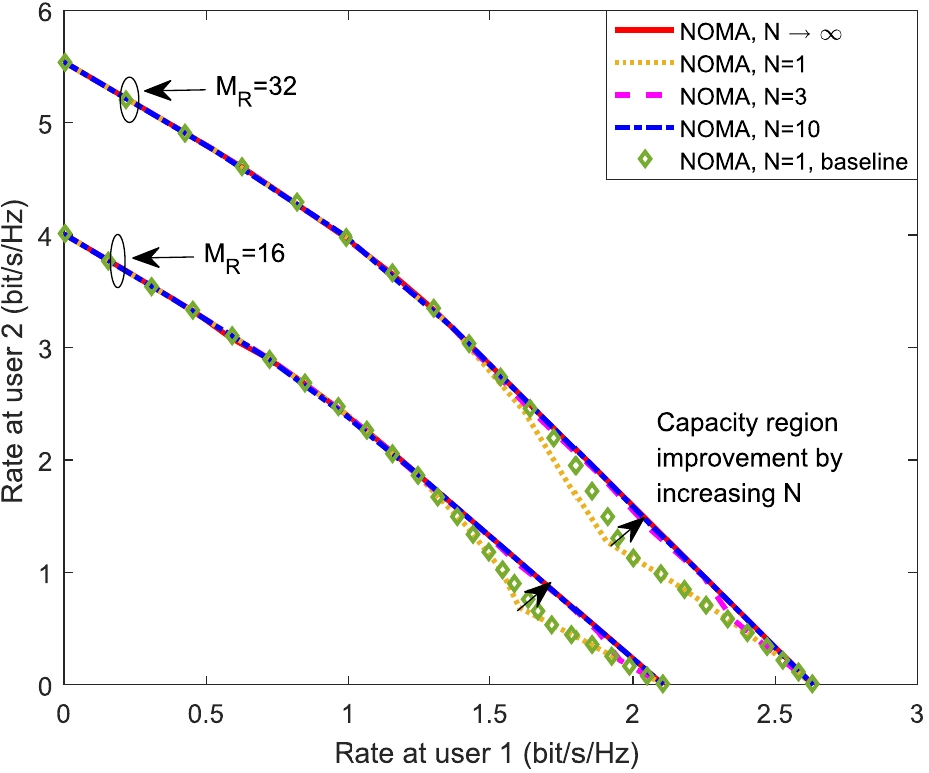
\includegraphics[scale=1]{../assets/viva/rate_region_noma.jpg}
						}
					}
					\subfloat{
						\resizebox{0.4\columnwidth}{!}{
							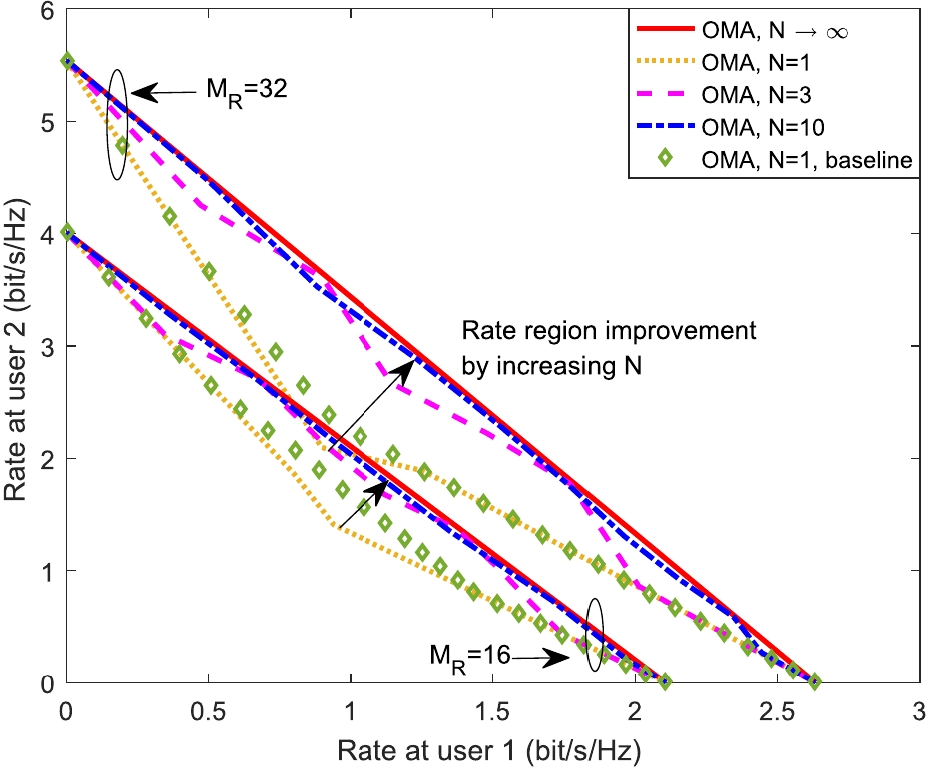
\includegraphics[scale=1]{../assets/viva/rate_region_oma.jpg}
						}
					}
				\end{figure}
				\item Common message can be embedded in $\theta$ to push the boundary
			\end{itemize}
		\end{block}
	\end{frame}

	\begin{frame}{Future works: IV}
		\begin{block}{Feasibility of interference alignment by \gls{ris}}
			\begin{align*}
				&\text{find} && \mathbf{\Theta} &&&\\
				&\text{s.t.} && \mathbf{H}^{[kj]} = \mathbf{H}_\mathrm{D}^{[kj]} + \mathbf{H}_\mathrm{B}^{[k]} \mathbf{\Theta} \mathbf{H}_\mathrm{F}^{[j]} = \mathbf{0}, &&& \forall j \neq k\\
				& && \mathrm{rank}(\mathbf{H}^{[kk]}) = d_k, &&& \forall k
			\end{align*}
			\begin{itemize}
				\item Necessary and sufficient feasibility conditions?
				\item How many scattering elements are required on expectation?
				\item Multi-sector \gls{bd}-\gls{ris} \cite{Li2023c}?
			\end{itemize}
		\end{block}
	\end{frame}

\end{section}
\bibliographystyle{IEEEtran}
\bibliography{../misc/library.bib}
\end{document}
